\RequirePackage{kvoptions-patch}
\documentclass[11pt,twoside]{scrartcl}
%\usepackage[ngerman]{babel}
\usepackage[T1]{fontenc}
\usepackage[utf8]{inputenc}
\usepackage{url}
\usepackage{hyperref}
\usepackage{lmodern} 
\usepackage{amsmath}
\usepackage{amssymb}
\usepackage{mathabx}
\usepackage{gauss}
\usepackage{graphicx}
\usepackage{pict2e}
\usepackage{curve2e}
\usepackage{tikz}
\usepackage{pgfplots}
\usepackage{xcolor,pgf}
\usepackage{pdflscape}
\usepackage{multirow}
\usepackage{array}
\newcolumntype{C}[1]{>{\centering\arraybackslash}p{#1}}
\usepackage[scaled=0.75]{luximono}
\usepackage{listings}
\lstset{
	numbers=left,
	numbersep=5pt,
	numberstyle=\tiny,
	language=C++,
	basicstyle=\small\ttfamily,
	keywordstyle=\bfseries,
	frame=shadowbox,
	columns=fullflexible,
	breaklines=true,
	float,
	tabsize=6,
	captionpos=b}
\usepackage[
	title={Development of a FEM code for fluid-structure coupling},
	author={Stephan Herb},
	type=master,
	institute=ipvs,
	number=39,
	course=cs,
	examiner={Prof.\ Dr.\ Miriam Mehl},
	supervisor={Dipl.-Ing.\ Florian Lindner},
	startdate={08.\ Juni 2015},
	enddate={08.\ Dezember 2015},
	crk={G.1.8, G.4, I.6}, 
    % http://www.acm.org/about/class/ccs98-html
	% G.1.8: Partial Differential Equations --> Finite Element Methods
	% G.4: Mathematical Software
	% I.6: Simulation and Modeling
	language=german %TODO cover und erklärung auf englisch oder deutsch
	%language=english
	]{uni-stuttgart-cs-cover}

\begin{document}
\Coverpage

\section*{Abstract}
% - Minimum halbe Seite bzw. 250-300 wörter
% - Was habe ich gemacht ... is presented.
% - vergleichaspekte erstellt und frameworks getestet, um am besten geignetes zu finden -> libMesh ist es geworden
% - Detailierter, welche Shell Elements, bestehen aus Plane und Plate
% - 2 Versionen: Tri und Quad, jeweils welches Modell
% - Programm entwickelt: eigenständige version und version mit einbindung von precice zur kopplung an multi-physics simulation. das programm kann mittels mpi parallel betrieben werden
% - details zur implementierung 
% - validierung der shell elements und ihrer komponenten durch viele tests. tests haben hohe genauigkeit in plane displacements gezeigt und ausreichend gute genauigkeit in plate displacements. die genauigkeit der shell elements ist akzeptabel aufgrund der einfachen approximation der elemente. die konvergenz-tests zeigen, dass bei ausreichend hoher unterteilung des meshs die genauigkeit sehr hoch ist.
% - das programm skaliert gut im parallelen
% - die kopplungstests/die validierung der kopplung hat gezeigt, dass das programm mittels precice erfolgreich an multi-physic simulationen gekoppelt werden kann

The development of a FEM structure solver for a coupled fluid-structure interaction simulation is presented in this thesis. Different aspects were created to evaluate existing FEM libraries. The libMesh framework was considered to be best suitable and was used in the development of the program. Two different discretizations of flat shell elements were implemented, a triangular and a quadrilateral element. The shell elements are constructed by the superposition of plane and plate elements. For the plane elements a model from XXX and XXX was used, the plate element's model is XXX and XXX. The developed program offers two versions, one coupled version to be used in a multi-physics simulation and a stand-alone version whose intention was to better validate the implemented finite elements. Both versions are parallelized with MPI. The coupling environment preCICE was used in the development of the coupled version. The validation of the elements showed good accuracy for the plane element components compared to analytical solutions as well as commercially available software. The plate element's accuracy is lower compared to the plane elements due to the chosen models that have a simpler approximation of the physical circumstances. The superimposed shell element's accuracy is well suited to be used in the structure solver. For both finite elements the accuracy can be increased arbitrarily by subdividing the mesh further. The parallelization test showed a good scaling with the number of processes for the assembly of the system's matrix and right-hand side as well as for the solving step. As an coupling example, a fluid-structure coupling between the developed program and a fluid solver developed with openFOAM was tested. The developed structure solver showed good performance in the simulation and is qualified for further multi-physics simulations connected via preCICE.
\newpage %TODO Abstract auch auf deutsch?
\cleardoublepage

\tableofcontents
\cleardoublepage

\section*{Abstract}
% - Minimum halbe Seite
% - Was habe ich gemacht ... is presented.
% - vergleichaspekte erstellt und frameworks getestet, um am besten geignetes zu finden -> libMesh ist es geworden
% - Detailierter, welche Shell Elements, bestehen aus Plane und Plate
% - 2 Versionen: Tri und Quad, jeweils welches Modell
% - Programm entwickelt: eigenständige version und version mit einbindung von precice zur kopplung an multi-physics simulation. das programm kann mittels mpi parallel betrieben werden
% - details zur implementierung 
% - validierung der shell elements und ihrer komponenten durch viele tests. tests haben hohe genauigkeit in plane displacements gezeigt und ausreichend gute genauigkeit in plate displacements. die genauigkeit der shell elements ist akzeptabel aufgrund der einfachen approximation der elemente. die konvergenz-tests zeigen, dass bei ausreichend hoher unterteilung des meshs die genauigkeit sehr hoch ist.
% - das programm skaliert gut im parallelen
% - die kopplungstests/die validierung der kopplung hat gezeigt, dass das programm mittels precice erfolgreich an multi-physic simulationen gekoppelt werden kann

Dieser Paragraph enthält eine nette kleine Zusammenfassung, in der zusammengefasst ist, was diese Arbeit enthält und tolles neues gemacht hat, das die Welt revolutionieren wird. Dieser Text hier dient im Augenblick nur als Platzhalter und wer ihn liest, sollte sich nicht beklagen, dass er oder sie gerade Zeit verschwendet hat.
\newpage

\section{Introduction}
Here comes the introduction$\ \ldots\ $ my worst nightmare.\newpage
% Batoz_et_al-1982 \cite{batoz1982evaluation} hat gute intro an der man schauen kann, wie man eine macht

% - einführende worte zu FEM -> see \cite{kansara2004development}
%
% - ziele und durchführung (ein bisschen den abstract wiederholen, aber keine ergebnisse mehr verraten)

\subsection{Organization}
% was gibt es in welchem kapitel für inhalt, quasi ein überblick über die arbeit ohne genaue details oder ergebnisse
\cleardoublepage

\section{Framework Evaluation}
Part of the thesis was to analyze several frameworks which ease the work with the finite element method. An evaluation of frameworks was done to select a suitable one for the given task. The evaluation's criteria are presented in this chapter together with a short description of the studied frameworks and a motivation for the library that were finally chosen.
 
 
 
 \subsection{General Aspects}
 In preparation of evaluating the frameworks many criteria were created in order to find the most suitable library. The individual aspects are as follows:
 \begin{itemize}
  \item Open Source: All frameworks under consideration need to be published under a free license that allows modification and redistribution. The implemented program should be used by anyone without requiring to purchase additional commercial software.
  
  \item Parallelization: Due to the need of accelerating calculations, the framework has to support an implementation of the widely used Message Passing Interface (MPI). The library should be able to use MPI internally for its own functions and procedures, but also support the developer with auxiliary function for communicating framework-related data.
 
  \item The programming language was chosen to be C++. This aspect is subjective and due to the individual experience of the author that is larger than, for example, with Python. It is not required that the framework is internally written in C++, but if not, it must provide an interface to C++ to work with.
 
  \item Mesh file import: Since the program should be able to work with complex geometries, the definition of such a mesh cannot be done in source code. Therefore, the library should provide a possibility to import meshes from file. The file must contain definitions of the node positions as well as the topology of the elements. Additionally, boundary conditions must be definable through identifiers at nodes or edges. The actual formats of the mesh files supported is not important, as long it supports the addressed requirements. A framework proprietary format would also be possible if it is simply reproducible.
  
  \item Linked to the previous aspect is the variety of different finite element types the library has to provide. The current program version uses triangles and quadrilaterals with three and four nodes, respectively. To be able to expand the program's functionality in the future, the library should support elements like six node triangles, nine node quadrilaterals or three dimensional elements like tetrahedra and hexahedra.
  
  \item Built-in solvers: The framework must provide a variety of different iterative solvers that can be interchanged at runtime by the user, or at least easily in the source code. Thus, the user has a higher flexibility when optimizing a problem or comparing different solvers in order to find the best for his or her problem. In the context of a structure solver for linear elastic problems it is focused especially on the group of linear iterative solvers.
 
  \item Accessible and detailed documentation: In order to guarantee maintainability and expandability the framework has to have a good documentation. This includes a complete documentation of every class and function, that is actively growing with the library itself. Additional documented example codes help the developer learning how to use the library correctly and efficiently. If problems with the framework occur the developer should be able to get in contact with the framework developers via mailing-lists or forums.
 
  \item Up-to-date: The framework should be well maintained and actively supported by its developers to ensure a long term compatibility with new features of the program code.
 
  \item The framework should be used by at least a few projects or has been part of publications. This shows the framework's importance and usability.
 
  \item Easy to learn syntax and structure: A rather subjective aspect, not less important. The developer should be able to concentrate more on the mathematical/physical problems and less on programming details. This accompanies the choice of the programming language as well as the documentation aspect.
 \end{itemize}
 
 
 
 \subsection{Frameworks Overview}
 The following list contains the FEM libraries which were evaluated in detail.
  
  %\subsubsection{FEniCS}
  
  \subsubsection{Feel++}
  Feel++ stands for "`Finite Element Embedded Language in C++"' and is a unified framework for finite and spectral Galerkin methods in 1D, 2D and 3D to solve partial differential equations \cite{prud2012feel++}. It was created in 2005 and is still actively maintained with daily commits and the last release version from February, 2015.
  One main aspect of Feel++ is to have syntax, semantics and pragmatics close to the mathematics. It allows creation of versatile mathematical kernels for testing and comparing different techniques and methods in solving problems. A second aim is to have a small library that is well manageable but makes use wherever possible of established libraries, for example to solve linear systems.
  It interfaces seamlessly with MPI simplifying the work's program parallelization. Different mesh file formats are available for import, like the GMSH format and a collection of different finite element types are supported.
  It is currently used in projects at Cemosis (Center for Modeling and Simulation in Strasbourg, France) including fluid structure interactions, high field magnets simulation and optical tomography \cite{feelpp}.

%%%%%%%%%%%%%%%%%%%%%% KORREKTUR-GRENZE %%%%%%%%%%%%%%%%%%%%%%%%%%%%%%%%%%%%%%

  \subsubsection{OOFEM}\cite{oofem}
  The "`Object Oriented Finite Element Method"' framework is an multi-physics finite element code with object oriented architecture \cite{patzak2001design}. The aim of is to provide an efficient and robust tool for FEM computations as well as to offer highly modular and extensible environment for development \cite{oofem}; extensible in terms of new element types, boundary conditions or numerical algorithms that can be created by the user. OOFEM focuses on efficient and robust solution to mechanical, transport and fluid problems providing corresponding modules for it. It is written in C++ with focus on high portability between platforms and interfaces various external software libraries like PETSc, ParMETIS, and ParaView. The last stable release were published on February, 2014 but it is still actively developed. The framework is used in several publications \cite{oofemPubs}.
  
  
  
  \subsubsection{GetFEM++}
  GetFEM++ is a generic finite element C++ library. It aims at providing finite element methods and elementary matrix computations for solving (non-)linear problems numerically. The user describes a model by gathering the variables, data and terms of a problem and some predefined bricks representing classical models. It allows easy switching from one method to another due to separation of geometric transformation or integration methods, for instance. It uses MPI for parallelization, though it is stated that "`a certain number of procedures are still remaining sequential"' \cite{getfemppMPI} at the time this work were written. While the framework is implemented in C++, it provides interfaces to languages like Python and Matlab. Thus, the framework can be handled by scripts written in non-C++ languages. The latest release is dated from July, 2015 with daily commits from the developers. GetFEM++ is used in project like IceTools \cite{icetools} (open source model for glaciers), EChem++ \cite{echempp} (Problem Solving Environment for Electochemistry) and SimNIBS \cite{simnibs} (software for Simulation of Non-invasive Brain Stimulation) and is part of some publications \cite{getfempp}.
  
  
  
  \subsubsection{MFEM}
  The ``Modular Finite Element Method'' library acts as a toolbox that provides the building blocks for developing finite element algorithms. MFEM aims to enable research and development of scalable finite element discretization and solver algorithms through general finite element abstractions. It has a wide variety of 2D and 3D finite element types, for example triangular and quadrilateral 2D elements, curved boundary elements or topologically periodic meshes. In addition to Galerkin methods, MFEM supports mixed finite elements, discontinuous Galerkin (DG) methods, or isogeometric analysis methods, for instance. The framework supports MPI-based parallelism throughout the library with minimal changes to the code to make the serial code parallel. A variety of solvers are available for the resulting linear algebra systems, including serial and parallel smoothers, solvers such as PCG, MINRES and GMRES, high-performance preconditioners from the hypre library,
  to name a few \cite{mfem}. The latest release of MFEM is dated January, 2015 but it is still under active development. The library is used in several publications \cite{mfemPubs}.
  
  
  
  
  \subsubsection{libMesh}\cite{kirk2006libmesh}
  The libMesh library provides a framework for the numerical simulation of partial differential equations using arbitrary unstructured discretizations on serial and parallel platforms. A major goal of the library is to provide support for adaptive mesh refinement (AMR) computations in parallel while allowing a research scientist to focus on the physics they are modeling. It makes use of existing software whenever possible. PETSc can be used for the solution of linear systems on both serial and parallel platforms, and LASPack is included with the library to provide linear solver support on serial machines, for instance. LibMesh supports a variety of 1D, 2D, and 3D geometric and finite element types and seamlessly integrates parallel functionality with MPI throughout the whole library \cite{kirk2006libmesh}. The framework is actively developed with daily commits and the latest release is dated from February, 2015. It is part of many publications \cite{libmeshPubs}.
  
  LibMesh was chosen to be the most suitable framework for this thesis. Its seamlessly integration of MPI reduces the effort of parallelization for the user, the required finite element types are supported and a range of many more are available for future expansions of the program's code. Complex geometries can be defined in several different mesh format as well as a simple libMesh particular format. The integration of external libraries like PETSc gives a high flexibility for users to change solvers and/or preconditioners. The library's classes and functions are well documented and a large collection of example codes are available. It is actively maintained by fixing bugs and adding more features. Although the structure and components of the framework are intuitive to understand, guided by the documentation, support by the developers are provided through mailing-lists.
  
% \subsection{Comparison}
\newpage
\cleardoublepage

\section{Shell Elements}\label{sec:Shell}
 Shell elements are used when structures need to be modeled where plane stresses as well as bending stresses are present. Different types of shell elements are available, including curved shell elements, shells of revolution, generalized shells or flat shell elements \cite{cook2002concepts}. The flat shell elements are subject of this work. Such an element can be constructed by the superposition of a plane and a plate element. This section contains the fundamentals of linear elastic problems - the field of application for the shell element - as well as the mathematical derivation of the plane and plate element, their combination resulting in the shell element and the necessary coordinate transformation that is needed for the implementation. 
 
 
 \subsection{Introduction to Linear Elastic Problems}\label{sec:Shell-IntroLinEla}
 In the following the fundamental equations of linear elasticity will be considered. Here, the spatial case is used for demonstration, but every lower dimensional problem can easily be derived from it.
 The following definitions will be used in this thesis:
 \begin{align}
 \vec{u} &= \begin{pmatrix}
 u & v & w
 \end{pmatrix}^T \text{displacement\ vector}
 \vec{f} &= \begin{pmatrix}
 f_x & f_y & f_z
 \end{pmatrix}^T \text{external\ force\ vector}
 \end{align}
 The strains and stresses can either be described in form of tensors $\underline{\varepsilon}$ and $\underline{\sigma}$, or as vectors $\vec{\varepsilon}$ and $\vec{\sigma}$:
 \begin{align}
 \underline{\varepsilon} &= \begin{pmatrix}
 \varepsilon_{xx} & \varepsilon_{xy} & \varepsilon_{xz} \\
 \varepsilon_{yx} & \varepsilon_{yy} & \varepsilon_{yz} \\
 \varepsilon_{zx} & \varepsilon_{zy} & \varepsilon_{zz} \end{pmatrix}\\
 \underline{\sigma} &= \begin{pmatrix}
 \sigma_{xx} & \sigma_{xy} & \sigma_{xz} \\
 \sigma_{yx} & \sigma_{yy} & \sigma_{yz} \\
 \sigma_{zx} & \sigma_{zy} & \sigma_{zz} \end{pmatrix}
 \end{align}
 \begin{align}
 \vec{\varepsilon} &= \begin{pmatrix}
 \varepsilon_{xx} & \varepsilon_{yy} & \varepsilon_{zz} & 2\varepsilon_{xy} & 2\varepsilon_{yz} & 2\varepsilon_{zx} \end{pmatrix}^T\\
 \vec{\sigma} &= \begin{pmatrix}
 \sigma_{xx} & \sigma_{yy} & \sigma_{zz} & \sigma_{xy} & \sigma_{yz} & \sigma_{zx} \end{pmatrix}^T
 \end{align}
 In the case of isotropic materials the strains and stresses are symmetrical, i.e. $\varepsilon_{xy} = \varepsilon_{yx}, \varepsilon_{xz} = \varepsilon_{zx}, \varepsilon_{yz} = \varepsilon_{zy}$ and $\sigma_{xy} = \sigma_{yx}, \sigma_{xz} = \sigma_{zx}, \sigma_{yz} = \sigma_{zy}$. As stated in \cite{steinke2005finite} the relation between displacements and strains is as follows:
 \begin{align}\label{eq:displ_strain_relation}
 \underline{\varepsilon} &= \frac{1}{2}\left(\nabla\vec{u} + \vec{u}\:\nabla \right) \\
 \vec{\varepsilon} &= \underline{L}\vec{u} \nonumber
 \end{align}
 Equation \eqref{eq:displ_strain_relation} relates the displacement vector field $\vec{u}$ with the strain field $\underline{\varepsilon}$, or $\vec{\varepsilon}$ respectively. Here, $\underline{L}$ is a differential operator. This strain-displacement relation is also called \textit{kinematic relationship} \cite{steinke2005finite}.
 
 In general initial strains can exist inside the material for example due to temperature changes or shrinkage. Such initial strains are denoted $\vec{\varepsilon_0}$ and the stresses will be influenced by the difference between the actual and initial strains. Additionally one could imagine initial residual stresses $\vec{\sigma_0}$ that can be added to the general equation:
 \begin{equation}\label{eq:stress-strain-relation}
 \vec{\sigma} = \underline{D}\left(\vec{\varepsilon}-\vec{\varepsilon_0}\right)+\vec{\sigma_0}
 \end{equation}
 where $\underline{D}$ is the material matrix. In the simplest case of linear elasticity with isotropy, $\underline{D}$ only contains two parameters, namely the elastic modulus $E$ (also known as the Young's modulus) and the Poisson's ratio $\nu$. The former one defines the relationship between the stress and strain in a material, the latter one results as the quotient of the fraction of expansion and the fraction of compression for small changes.
 
 In the following the initial conditions are ignored, resulting in the a simpler form of equation \eqref{eq:stress-strain-relation}:
 \begin{equation}
 \vec{\sigma} = \underline{D}\ \vec{\varepsilon}
 \end{equation}
 For the said isotropic case $\underline{D}$ results in \cite{zienkiewicz2000finite}:
 \begin{equation}
 \underline{D} = \frac{E}{1-\nu^2}\begin{pmatrix}
 1 & \nu & 0 \\
 \nu & 1 & 0 \\
 0 & 0 & \frac{1-\nu}{2}
 \end{pmatrix}
 \end{equation}
 
 The equilibrium conditions as described in \cite{steinke2005finite}, are as follows:
 \begin{equation}\label{eq:equilibrium-conditions}
 \underline{L} \vec{\sigma} + \vec{b} = \vec{0}
 \end{equation}
 where the vector $\vec{b}$ describes internal volume forces and $\vec{0}$ is the zero vector.
 
 Two different boundary conditions are distinguished: Essential and natural boundary conditions. The first one is geometrically described. An initial displacement $\vec{u^0}$ is impressed on a surface part $\Omega_u$ of the object:
 \begin{equation}
 \vec{u} = \vec{u^0}\quad \text{on}\quad \Omega_u
 \end{equation}
 The natural boundary conditions are represented by force conditions. They can be described as follows:
 \begin{equation}
 \underline{n} \vec{\sigma} = \vec{p^0}\quad \text{on}\quad \Omega_p
 \end{equation}
 where the matrix $\underline{n}$ contains entries of the object boundary's normal vector, $\vec{p^0}$ described the edge stress and $\vec{\sigma}$ is the stress vector:
 \begin{align}
 \vec{n} &= \begin{pmatrix}
 n_x\\n_y\\n_z
 \end{pmatrix}\\
 \underline{n} &= \begin{pmatrix}
 n_x & 0 & 0 & n_y & 0 & n_z\\
 0 & n_y & 0 & n_x & n_z & 0\\
 0 & 0 & n_z & 0 & n_y & n_x
 \end{pmatrix}
 \end{align}
 
 In \cite{steinke2005finite} the principle of the total potential for the fundamental equations of linear elasticity is illustrated. Initial point is the weak formulation of the equilibrium conditions \eqref{eq:equilibrium-conditions} for a body $V$:
 \begin{equation}
 \int_{V} \left(\underline{L} \vec{\sigma} + \vec{b}\right) \vec{\lambda}\ dV = 0
 \end{equation}
 The introduction of Lagrange multipliers $\vec{\lambda}$ leads to a weighting and can be expressed as variation of $\delta \vec{u} = \vec{\lambda}$. The result of the derivation of the above equation is the expression of the total potential $\Pi$:
 \begin{equation}
 \Pi = \frac{1}{2} \int_{V} \vec{\sigma}^T \vec{\varepsilon}\ dV - \left(\int_{V}\vec{b}^T \vec{u}\ dV - \int_{\Omega_p} \vec{p^0}^T \vec{u}\ d\Omega_p\right) = \Pi_D - \Pi_e
 \end{equation}
 The first term describes the elastic deformation energy $\Pi_D$, the two terms in brackets combine the potential of the external forces $\Pi_e$
 
 \subsection{Plane Element}\label{sec:Shell-Plane}
  Plane elements are characterized by that loads are only apply in the mid-surface directions of an element and all displacements, strains and stresses happen in the mid-surface, too. In this section plane elements are discussed in more detail and two different discretizations, a three-node triangular element and a four-node quadrilateral element, are described.
  
  
  \subsubsection{Problem Definition}\label{sec:Shell-Plane-ProbDef}
  \begin{figure}[htbp]%- Bild ähnlich ch7.1 mit xy-Ausdehnung, Dicke t, Mittelfläche, Rand, KoSys; Streckenlast q0 und Volumenkraft g aber weglassen
\centering
%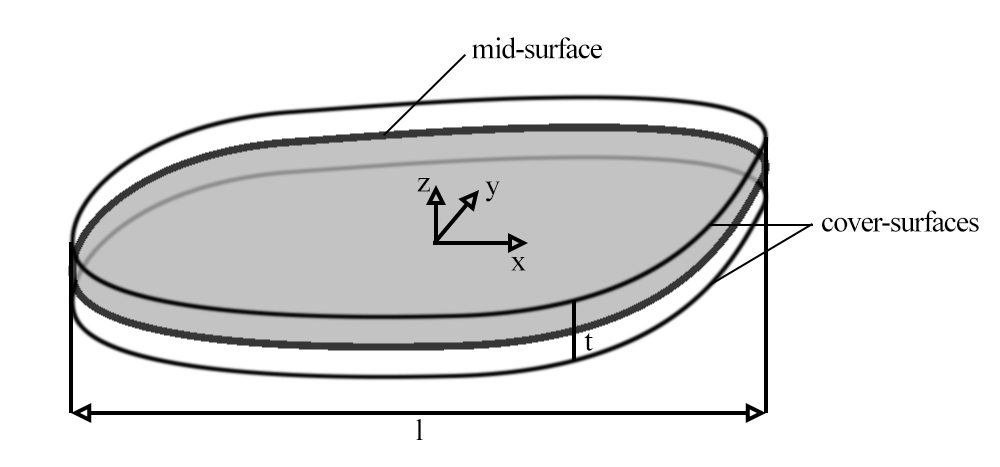
\includegraphics[width=0.97\linewidth]{figures/plane}
\setlength\unitlength{1.0cm}
\begin{picture}(12,6)
\thinlines
\put(0,0){\pgfsetfillopacity{1.0}\Curve(0.5,2.5)<0,0.25>(3.5,4.25)<1,0.125>(7.5,4.5)<1,0>(10,2.5)<-1,-1>(6,1)<-0.5,-0.05>(2.5,1)<-0.5,0.125>(0.5,2.5)<0,0.5>}
\thicklines
{\pgfsetfillopacity{0.8}\color{gray}\Curve*(0.5,3)<0,0.25>(3.5,4.75)<1,0.125>(7.5,5)<1,0>(10,3)<-1,-1>(6,1.5)<-0.5,-0.05>(2.5,1.5)<-0.5,0.125>(0.5,3)<0,0.5>}
\put(0,0){\pgfsetfillopacity{1.0}\color{black}\Curve(0.5,3)<0,0.25>(3.5,4.75)<1,0.125>(7.5,5)<1,0>(10,3)<-1,-1>(6,1.5)<-0.5,-0.05>(2.5,1.5)<-0.5,0.125>(0.5,3)<0,0.5>}
\put(6.6,2.9){$x$}
\put(5.5,3){\vector(1,0){1}}
\put(6.1,3.4){$y$}
\put(5.5,3){\vector(0.5,0.65){0.5}}
\put(5.4,4.1){$z$}
\put(5.5,3){\vector(0,1){1}}
\thinlines
\put(0,0){\pgfsetfillopacity{1.0}\Curve(0.5,3.5)<0,0.25>(3.5,5.25)<1,0.125>(7.5,5.5)<1,0>(10,3.5)<-1,-1>(6,2)<-0.5,-0.05>(2.5,2)<-0.5,0.125>(0.5,3.5)<0,0.5>}
\Dline(0.5,3.5)(0.5,0.5){0.1}
\Dline(10.37,3.5)(10.37,0.5){0.1}
\put(5,0.5){\vector(-4.5,0){4.5}}
\put(5,0.5){\vector(5.37,0){5.37}}
\put(5.4,0.15){$l$}
\Line(2.5,2)(2.5,1)\put(2.43,0.7){$t$}
\polyline(10,3.5)(11,3)(10,2.5)\put(11.1,2.9){cover-surfaces}
\Line(7.5,5)(9.5,5.5)\put(9.6,5.4){mid-surface}
\end{picture}
\caption{Schematic view of a plane object with main dimension $l$ and thickness $t$. The two cover-surfaces are located at $z=\pm \frac{t}{2}$, the mid-surface at $z=0$.}
\label{fig:plane}
\end{figure}
  In Figure \ref{fig:plane} an object is shown which extends to the x and y axis as its primary direction. The extend in z-direction is smaller and denoted by thickness $t$. The mid-surface located in between the top and bottom surface areas has the coordinate $z=0$. Its local z-axis equals the normal vector of the mid place. Such an object is called \textit{plane} in the following.
  
  %- Bed. für ebenen Spannungszustand (eb. Dehnungszustand erwähnen und auf Ref (z.B. Zienkiewicz) verweisen)
  There are two different formulations regarding plane elements: Plane stress and plane strain. The directions of displacements $u$ and $v$ along the orthogonal local x and y axis defining its displacement field is a common feature of both problems. Also, both have in common, that only strains and stresses in the xy plane have to be considered: Instead of nine, only three components remain. While in the case of plane stress all other stress components are zero, in plane strain the stress in direction perpendicular to the xy plane is non-zero. In this thesis only plane stress will be discussed in further detail. More information about plane strain is given in \cite{zienkiewicz2000finite} and \cite{braess2007finite}, for instance.
  The following conditions must be satisfied such that a plane can be in \textit{plane stress} \cite{steinke2005finite}:
  \begin{itemize}
  	\item The thickness $t$ varies only slightly and it must hold: $t/l \ll 1$, with $l$ the extent of the larger side of the plane element.
  	\item The load is applied to the mid-surface.
  	\item Displacements, strains and stresses are constant across the thickness.
  \end{itemize}
  The stress components $\sigma_{xz},\sigma_{yz},\sigma_{zz}$ normal to the surface areas with $z \pm t/2$ vanish (equals zero). Therefore only the two normal stress components $\sigma_{xx}$ and $\sigma_{yy}$ and the transverse stress component $\sigma_{xy}$ are left non-zero.
    
  %- Verschiebungen, Dehnungen und Spannungen beschreiben + kinematische Beziehung + Stoffgleichung\newline
  Displacements can only occur in x and y direction. $u$ will be the displacement along x and $v$ along y. The displacement field $\vec{u}$ is as follows:
  \begin{equation}
  \vec{u}=\begin{pmatrix}
  u(x,y) & v(x,y)
  \end{pmatrix}^T
  \end{equation}
  The vector for the strain components:
  \begin{equation}
  \vec{\varepsilon}=\begin{pmatrix}
  \varepsilon_{xx} & \varepsilon_{yy} & 2\varepsilon_{xy}
  \end{pmatrix}^T
  \end{equation}
  Sometimes $2\varepsilon_{xy}$ is shortened to $\gamma_{xy}$ \cite{steinke2005finite}.
  The vector holding the stress components is similar to that of the strain's vector:
  \begin{equation}
  \vec{\sigma}=\begin{pmatrix}
  \sigma_{xx} & \sigma_{yy} & \sigma_{xy}
  \end{pmatrix}^T
  \end{equation}
  The kinematic relationship $\vec{\varepsilon}=\underline{L}\vec{u}$ (eq.\ \eqref{eq:displ_strain_relation}) linking the displacements $\vec{u}$ with the strains $\vec{\varepsilon}$ can be written at full length:
  \begin{equation}\label{eq:t3displ-str-rel}
  \vec{\varepsilon} = \begin{pmatrix}
  \varepsilon_{xx} \\
  \varepsilon_{yy} \\
  2\varepsilon_{xy}
  \end{pmatrix} =
  \begin{pmatrix}
  \frac{\partial u}{\partial x} \\
  \frac{\partial v}{\partial y} \\
  \frac{\partial u}{\partial y} + \frac{\partial v}{\partial x}
  \end{pmatrix} =
  \begin{pmatrix}
  \frac{\partial}{\partial x} & 0 \\
  0 & \frac{\partial}{\partial y} \\
  \frac{\partial}{\partial y} & \frac{\partial}{\partial x}
  \end{pmatrix}
  \begin{pmatrix}
  u \\
  v
  \end{pmatrix}
  = \underline{L} \vec{u}
  \end{equation}
  With the strains known and considering equation \eqref{eq:displ_strain_relation} one can calculate the stresses $\vec{\sigma}$:
  \begin{equation}\label{eq:sigma=D*eps}
  \vec{\sigma} = \begin{pmatrix}
  \sigma_{xx} \\
  \sigma_{yy} \\
  \sigma_{xy}
  \end{pmatrix} = \frac{E}{1-\nu^2} \begin{pmatrix}
  1 & \nu & 0 \\
  \nu & 1 & 0 \\
  0 & 0 & \frac{1-\nu}{2}
  \end{pmatrix} \begin{pmatrix}
  \varepsilon_{xx} \\
  \varepsilon_{yy} \\
  2\varepsilon_{xy}
  \end{pmatrix} = \underline{D} \vec{\varepsilon} = \underline{D}\; \underline{L} \vec{u}
  \end{equation}
  %- Randbedingungen: q0 Streckenlast beschreiben, aber angeben, dass sie hier nicht beachtet werden, punktf. Ladungen werden hier benutzt\newline

  After Steinke \cite{steinke2005finite}, the essential boundary conditions $\vec{u} = \vec{u^0}$ and the natural boundary conditions $t\ \underline{n}\ \vec{\sigma} = \vec{q^0}$ will be applied onto the objects boundary $\Gamma$, with $t$ is the object's thickness and $\vec{q^0}$ represents a line load. The matrix $\underline{n}$ looks as follows \cite{steinke2005finite}:
  \begin{equation}
  \underline{n} = \begin{pmatrix}
  n_x & 0 & n_y\\ 0 & n_y & n_x
  \end{pmatrix}
  \end{equation}
  Beside line loads, nodal forces $\vec{F} = \begin{pmatrix}
  F_x & F_y
  \end{pmatrix}^T$ are also possible.
  
  The total potential of the plane element problem looks as follows \cite{steinke2005finite}:
  \begin{equation}
  \Pi = \frac{1}{2} \int_{V}\vec{\varepsilon}^T\vec{\sigma}dV - \int_{V} \vec{u}^T \vec{b}\ dV - \int_{\Gamma_q}\vec{u}^T \vec{q}\ d\gamma -\vec{u}^T \vec{F}
  \end{equation}
  The first term describes the elastic strain energy, the last three terms describe the different external forces. The first of the three describes the potential of the volume forces $\vec{b}^T = \rho \begin{pmatrix}
  g_x & g_y
  \end{pmatrix}$, where $\rho$ is the object's density and $g_x, g_y$ represents accelerations in the two directions. The second term stands for the line load along an edge $\Gamma_q$ and the last term contains the single nodal forces.
  
  The external forces are summarized in this work to the last term only. Line loads and volume forces can be converted to nodal load, assuming a linear distribution over the edges and the interior of the element, respectively \cite{steinke2005finite}. Therefore, the total potential of the plane element shrinks to the following:
  \begin{equation}\label{eq:planeFunctional}
  \Pi = \frac{1}{2} \int_{V}\vec{\varepsilon}^T\vec{\sigma}dV - \vec{u}^T \vec{F}
  \end{equation}
  
  
  
  
  
  
  
  
  \subsubsection{Tri-3 Plane Element}\label{sec:Shell-Plane-Tri}
  In section \ref{sec:Shell-Plane-ProbDef} the plane element's functional was derived (eq. \eqref{eq:planeFunctional}). Now the focus is on the functional's discretization. The constructed finite element will be a three-node triangular element in the following also denoted as \textbf{Tri-3}. Figure \ref{fig:plane_triangulation} shows a general, planar object defined to be placed in the xy-plane. The first discretization step is to divide the object into single triangles approximating the shape of it. This process is called triangulation. Every one of these triangles then represents a finite element with one node at every corner. The finer the triangulation is done the better the object and its boundary are matched by its discrete complement, but also the more finite elements have to be considered in later calculations.
  \begin{figure}[htbp]% Bild von trianguliertem Körper
    	\centering
    	%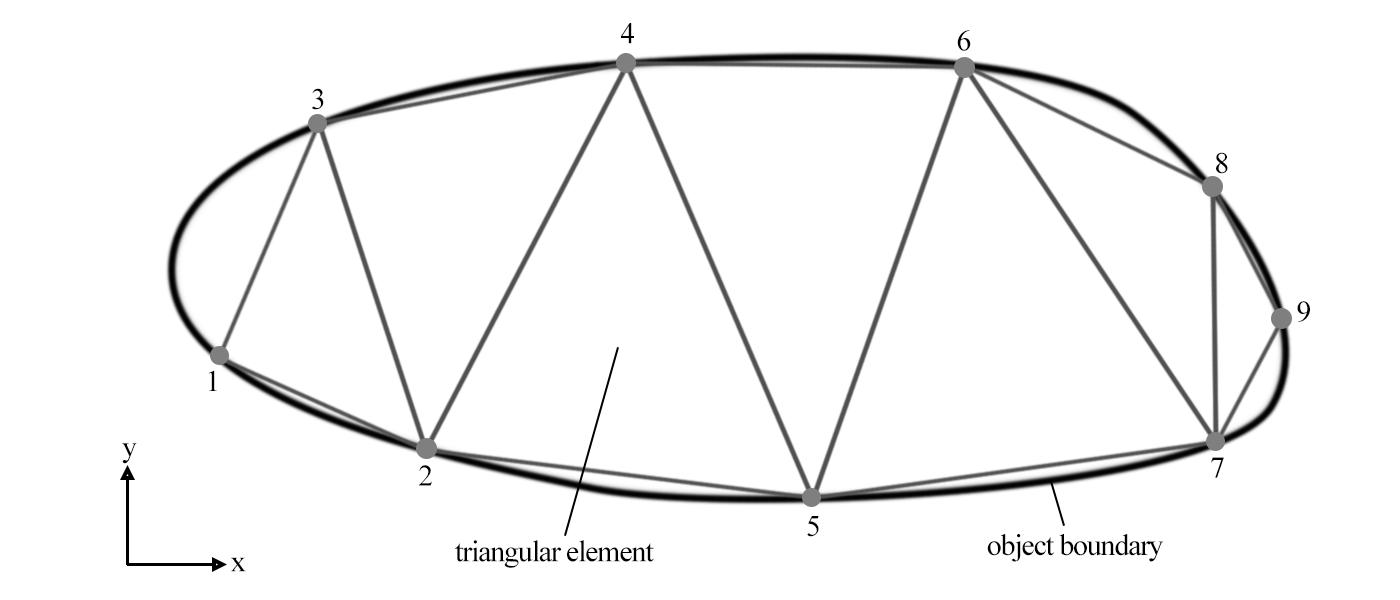
\includegraphics[width=1.0\linewidth]{figures/plane_triangulation}
    	\setlength\unitlength{0.9cm}
    	\begin{picture}(14,6)
    	\thicklines
    	\put(0.2,0.1){\vector(1,0){1.5}}
    	\put(0.2,0.1){\vector(0,1){1.5}}
    	\put(1.8,0){$x$}
    	\put(0.1,1.7){$y$}
    	
    	\put(1, 2.5){\cbezier(0,0)(0,0.5)(0.5,1.5)(2,2)}
    	\put(3,4.5){\cbezier(0,0)(1.5,0.5)(2.5,0)(3,0.5)}
    	\put(6,5){\cbezier(0,0)(0.5,0.5)(1.5,0.5)(3.5,0.5)}
    	\put(9.5,5.5){\cbezier(0,0)(2,0)(3,-1)(3.5,-2)}
    	\put(13,3.5){\cbezier(0,0)(0.5,-1)(-0.5,-2)(-2,-2)}
    	\put(11,1.5){\cbezier(0,0)(-1.5,0)(-2.5,0.5)(-3.5,1)}
    	\put(7.5,2.5){\cbezier(0,0)(-1,0.5)(-2.5,0)(-3.5,-1)}
    	\put(4,1.5){\cbezier(0,0)(-1,-1)(-3,0.5)(-3,1)}
    	\thinlines
    	\polyline(1,2.5)(3,4.5)(6,5)(9.5,5.5)(13,3.5)(11,1.5)(7.5,2.5)(4,1.5)(1,2.5)
    	\polyline(3,4.5)(4,1.5)(6,5)(7.5,2.5)(9.5,5.5)(11,1.5)(13,3.5)
    	\put(0.5,5.5){object boundary} \polyline(2,5.2)(1.65,3.7)
    	\put(6,1){triangular element} \polyline(8,1.5)(9.2,3)
    	\put(0.6,2.3){$1$}
    	\put(4.0,1.1){$2$}
    	\put(2.85,4.6){$3$}
    	\put(7.3,2.1){$4$}
    	\put(5.8,5.1){$5$}
    	\put(9.4,5.6){$6$}
    	\put(10.85,1.05){$7$}
    	\put(13.2,3.4){$8$}
    	\end{picture}
    	\caption{A plane object is partitioned into several triangular elements. This process is called triangulation.}
    	\label{fig:plane_triangulation}
  \end{figure}
    
  \begin{figure}[htbp]
  	\centering
  	%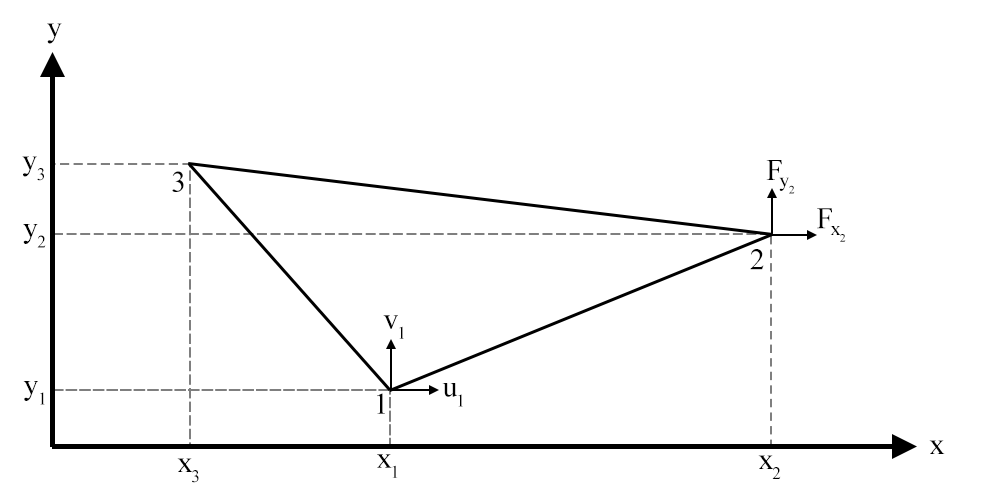
\includegraphics[width=1.0\linewidth]{figures/plane_triangle}
  	\setlength\unitlength{0.9cm}
	\begin{picture}(14,6)
	\thicklines
	\put(0.4,0.3){\vector(1,0){13.5}}
	\put(0.4,0.3){\vector(0,1){5.5}}
	\put(14.0,0.2){$\mathbf{x}$}
	\put(0.3,5.9){$\mathbf{y}$}
	
	\put(6.2,0.7){\line(6,2.5){6}}
	\put(5.85,0.35){$1$}
	\put(12.2,3.2){\line(-10,1){10}}
	\put(12.3,2.8){$2$}
	\put(2.2,4.2){\line(4,-3.5){4}}
	\put(1.9,3.8){$3$}
	
	\thinlines
	\Dline(6.2,0.7)(6.2,0.3){0.1}
	\put(6,0){$x_1$}
	\Dline(6.2,0.7)(0.4,0.7){0.1}
	\put(0,0.6){$y_1$}
	\Dline(12.2,3.2)(12.2,0.3){0.1}
	\put(12,0){$x_2$}
	\Dline(12.2,3.2)(0.4,3.2){0.1}
	\put(0,3.1){$y_2$}
	\Dline(2.2,4.2)(2.2,0.3){0.1}
	\put(2,0){$x_3$}
	\Dline(2.2,4.2)(0.4,4.2){0.1}
	\put(0,4){$y_3$}
	
	\put(6.2,0.7){\vector(1,0){1}}
	\put(7.3,0.6){$u_1$}
	\put(6.2,0.7){\vector(0,1){1}}
	\put(6.0,1.8){$v_1$}
	
	\put(12.2,3.2){\vector(1,0){1}}
	\put(13.3,3.1){$F_{x_2}$}
	\put(12.2,3.2){\vector(0,1){1}}
	\put(12.0,4.3){$F_{y_2}$}
	\end{picture}
  	\caption{A three-node triangular element is shown with its coordinates projected onto the axes. For the first node its nodal displacements and for the second node its nodal forces are exemplarily illustrated.}
  	\label{fig:plane_triangle}
  \end{figure}
    
  One triangular finite element is shown in Figure \ref{fig:plane_triangle}. It is defined by the coordinates $(x_i,y_i)$ of its three nodes. Since the element is located in the xy-plane, the z-coordinate is of no interest and will be ignored. At every node, forces can be applied denoted with $F_{x_i}$ and $F_{y_i}$. Accordingly, every node can be displaced. The movement along the x-axis is denoted with $u_i$ and with $v_i$ along the y-axis, respectively. Note, that the node numbering is in anti-clockwise direction. This convention will be kept throughout the thesis, and is important when implementing the FEM-code.
  In this thesis only triangles defined by three nodes are discussed. There are many more finite elements forming triangles, such as six node triangles or even seven node triangles. The main difference between these types of elements are the order of shape functions. More details about higher order triangular finite elements can be found in \cite{zienkiewicz2000finite}, \cite{bergan1985triangular}, \cite{cook2002concepts}, \cite{braess2007finite}.
  
  % ansatzfunktion (abgewandelt statt phi, u und v separat)\\
  In the case of a three node triangle the basis functions for the two displacements $u$ and $v$ are the same and thus $u$ and $v$ can be replaced by an arbitrary function $\psi$\cite{steinke2005finite}:
  \begin{align}\label{eq:t3_ansatz}
  \psi(x,y) &= a_0 + a_1L_1 + a_2L_2 = \begin{pmatrix}
  1 & L_1 & L_2
  \end{pmatrix} \begin{pmatrix}
  a_0 \\ a_1 \\ a_2
  \end{pmatrix} = \vec{x}^T \vec{a}
  \end{align}
  defined in triangular coordinates (see Figure \ref{fig:tri_coords}).
  
  \begin{figure}[htbp]% dreieckskoordinaten (ähnlich bild 2.7 auf s.39(53))
  	\centering
  	%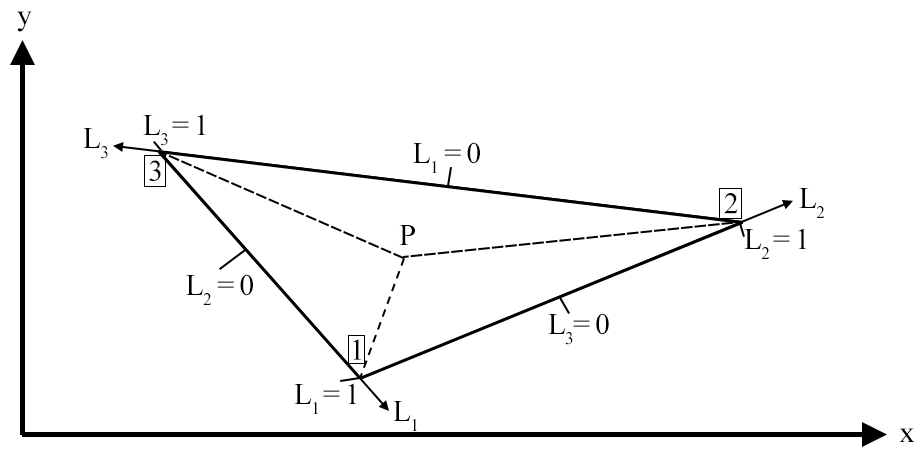
\includegraphics[width=0.9\linewidth]{figures/triangular_coords}
	\setlength\unitlength{0.9cm}
	\begin{picture}(14,6)
	\thicklines
	\put(0.4,0.3){\vector(1,0){13.5}}
	\put(0.4,0.3){\vector(0,1){5.5}}
	\put(14.0,0.2){$\mathbf{x}$}
	\put(0.3,5.9){$\mathbf{y}$}
	
	\put(6.2,0.7){\line(6,2.5){6}}
	\put(6.05,0.8){$1$}
	\put(12.2,3.2){\line(-10,1){10}}
	\put(12,3.3){$2$}
	\put(2.2,4.2){\line(4,-3.5){4}}
	\put(1.9,3.8){$3$}
	
	\thinlines
	\Dline(6.2,0.7)(6.5,2.5){0.1}
	\Dline(12.2,3.2)(6.5,2.5){0.1}
	\Dline(2.2,4.2)(6.5,2.5){0.1}
	\put(6.3,2.7){$P$}
	
	\put(12.2,3.2){\vector(6,2.5){0.5}}
	\put(12.8,3.3){$L_2$}
	\put(12.2,2.8){$L_2 = 1$}
	\put(6.2,0.7){\vector(4,-3.5){0.5}}
	\put(6.7,0.4){$L_1$}
	\put(4.9,0.4){$L_1 = 1$}
	\put(2.2,4.2){\vector(-10,1){0.7}}
	\put(1.0,4.2){$L_3$}
	\put(2.2,4.4){$L_3 = 1$}
	
	\put(9,1.5){$L_3 = 0$}
	\put(2.8,2.2){$L_2 = 0$}
	\put(7,4){$L_1 = 0$}
	\end{picture}
  	\caption{Triangular coordinates $L_1,L_2,L_3$ and sampling point $P$ within a triangular element. The nodes and edges represent special cases of triangular coordinates.}
  	\label{fig:tri_coords}
  \end{figure}
  
  % interpolationsbedingunen führen auf Formfunktionen\\
  To get the unknown coefficients $a_i$, values for the triangular coordinates are set. This creates a system of linear equations:
  \begin{align}
  \psi(L_1=1, L_2=0) = \psi_1 &\rightarrow \psi_1 = a_0 + a_1 \nonumber\\
  \psi(L_1=0, L_2=1) = \psi_2 &\rightarrow \psi_2 = a_0 + a_2 \nonumber\\
  \psi(L_1=0, L_2=0) = \psi_3 &\rightarrow \psi_3 = a_0
  \end{align}
  Written as matrix and vector:
  \begin{align}
  \underline{A} \vec{a} &= \vec{\psi} \nonumber\\
  \begin{pmatrix}
  1 & 1 & 0\\
  1 & 0 & 1\\
  1 & 0 & 0
  \end{pmatrix} \begin{pmatrix}
  a_0 \\ a_1 \\ a_2
  \end{pmatrix} &= \begin{pmatrix}
  \psi_1 \\ \psi_2 \\ \psi_3
  \end{pmatrix}
  \end{align}
  Now, inverting matrix $A$ the coefficients can be found:
  \begin{equation}\label{eq:t3_coeffsA}
  \vec{a} = \underline{A}^{-1} \vec{\psi} = \begin{pmatrix}
  0 & 0 & 1\\
  1 & 0 & -1\\
  0 & 1 & -1
  \end{pmatrix} \begin{pmatrix}
  \psi_1 \\ \psi_2 \\ \psi_3
  \end{pmatrix}
  \end{equation}
  If one put equation \eqref{eq:t3_coeffsA} into \eqref{eq:t3_ansatz}, the shape functions for the three node triangular finite element will be derived, as described in \cite{steinke2005finite}:
  \begin{align}\label{eq:t3SF}
  u &= \vec{x}^T \vec{a} = \vec{x}^T \underline{A}^{-1}\vec{u} = \vec{N}^T\vec{u} \nonumber\\
  \vec{N}^T &= \vec{x}^T \underline{A}^{-1} =
  \begin{pmatrix}
  1 & L_1 & L_2
  \end{pmatrix} \begin{pmatrix}
  0 & 0 & 1\\
  1 & 0 & -1\\
  0 & 1 & -1
  \end{pmatrix} \nonumber\\
  &= \begin{pmatrix}
  L_1 & L_2 & 1-L_1-L_2
  \end{pmatrix} = \begin{pmatrix}
  N_1 & N_2 & N_3
  \end{pmatrix}
  \end{align}
  Characteristically for a shape functions $N_i$ is, as stated in \cite{steinke2005finite}, that it evaluates to 1 at node $i$ and to 0 at the two other nodes. The functions are linear with respect to $L_1$ and $L_2$ which can be noticed in equation \eqref{eq:t3SF}. As stated before, these shape functions are the same for displacement $u$ and $v$. With the knowledge of the displacement values of the element's nodes one can formulate the displacement functions in triangular coordinate notation as follows:
  \begin{align}
  u &= N_1 u_1 + N_2 u_2 + N_3 u_3 \nonumber\\
  v &= N_1 v_1 + N_2 v_2 + N_3 v_3
  \end{align}
  Or in matrix form:
  \begin{align} \label{eq:t3u=Nu}
  \vec{\tilde{u}} &= \underline{N} \vec{u} \nonumber\\
  \begin{pmatrix}
  u \\ v
  \end{pmatrix} &= \begin{pmatrix}
  N_1 & 0 & N_2 & 0 & N_3 & 0 \\
  0 & N_1 & 0 & N_2 & 0 & N_3
  \end{pmatrix} \begin{pmatrix}
  u_1 \\ v_1 \\ u_2 \\ v_2 \\ u_3 \\ v_3
  \end{pmatrix}
  \end{align}
  The vector $\vec{\tilde{u}}$ describes the element's displacements as product of matrix $\underline{N}$ containing the shape functions and vector $\vec{u}$ containing the displacements of the single triangle's nodes. Now, one can put equation \eqref{eq:t3u=Nu} into \eqref{eq:t3displ-str-rel}:
  \begin{equation}\label{eq:t3eps=Bu}
  \vec{\varepsilon} = \underline{L}\vec{\tilde{u}} = \underline{L}\;\underline{N} \vec{u} = \underline{B} \vec{u}
  \end{equation}
  The product of $\underline{L}$ and $\underline{N}$ is called \textit{strain-displacement matrix} $\underline{B}$.
  In order to calculate the strain-displacement matrix, one has to assemble the $\underline{L}$ matrix containing the first partial derivatives of the triangular element. With the chain rule applied, the partial derivatives look as follows:
  \begin{align}
  \frac{\partial}{\partial L_1} = \frac{\partial x}{\partial L_1} \frac{\partial}{\partial x} + \frac{\partial y}{\partial L_1} \frac{\partial}{\partial y} \nonumber\\
  \frac{\partial}{\partial L_2} = \frac{\partial x}{\partial L_2} \frac{\partial}{\partial x} + \frac{\partial y}{\partial L_2} \frac{\partial}{\partial y}
  \end{align}
  or in matrix notation:
  \begin{align}\label{eq:t3NablaTilde}
  \tilde{\nabla} &= \underline{J} \nabla \nonumber\\
  \begin{pmatrix}
  \frac{\partial}{\partial L_1}\\ \frac{\partial}{\partial L_2}
  \end{pmatrix} &= \begin{pmatrix}
  \frac{\partial x}{\partial L_1} & \frac{\partial y}{\partial L_1}\\
  \frac{\partial x}{\partial L_2} & \frac{\partial y}{\partial L_2}
  \end{pmatrix} \begin{pmatrix}
  \frac{\partial}{\partial x}\\ \frac{\partial}{\partial y}
  \end{pmatrix},
  \end{align}
  where $\underline{J}$ represents the Jacobian matrix, $\nabla$ the partial derivatives in Cartesian coordinates and $\tilde{\nabla}$ the partial derivatives in triangular coordinates. To get the derivatives in Cartesian form the upper equation must be multiplied with the inverse Jacobian matrix $\underline{J}^{-1}$:
  \begin{equation}
  \underline{J}^{-1} = \frac{1}{|\underline{J}|} \begin{pmatrix}
  \frac{\partial y}{\partial L_2} & -\frac{\partial y}{\partial L_1} \\
  \frac{-\partial x}{\partial L_2} & \frac{\partial x}{\partial L_1}
  \end{pmatrix}
  \end{equation}
  where $|\underline{J}|$ denotes the determinant of the Jacobian matrix. The conversion between triangular and Cartesian coordinates can be summarized as follows (see Figure \ref{fig:tri_coords} and \cite{steinke2005finite}):
  \begin{align}\label{eq:triCoord<->CartCoord}
  L_1 + L_2 + L_3 &= 1 \rightarrow L_3 = 1-L_1-L_2 \nonumber\\
  x &= x_1L_1 + x_2L_2 + x_3L_3 = (x_1-x_3)L_1 + (x_2-x_3)L2 + x_3\\
  y &= y_1L_1 + y_2L_2 + y_3L_3 = (y_1-y_3)L_1 + (y_2-y_3)L2 + y_3 \nonumber
  \end{align}
  Considering equation \eqref{eq:triCoord<->CartCoord} the Jacobian matrix can now be calculated:
  \begin{equation}
  J = \begin{pmatrix}
  \frac{\partial x}{\partial L_1} = x_1-x_3 = x_{13} & \frac{\partial y}{\partial L_1} = y_1-y_3 = y_{13}\\
  \frac{\partial x}{\partial L_2} = x_2-x_3 = x_{23} & \frac{\partial y}{\partial L_2} = y_2-y_3 = y_{23}
  \end{pmatrix} = \begin{pmatrix}
  x_{13} & y_{13}\\
  x_{23} & y_{23}
  \end{pmatrix}
  \end{equation}
  and hence the inverse Jacobian matrix:
  \begin{equation}\label{eq:t3invJac}
  \underline{J}^{-1} = \frac{1}{2 A_\triangle} \begin{pmatrix}
  y_{23} & -y_{13}\\
  -x_{23} & x_{13}
  \end{pmatrix}
  \end{equation}
  The determinant of the Jacobian matrix is two times the area of the triangle. With the help of equation \eqref{eq:t3invJac}, \eqref{eq:t3NablaTilde} can be reorganized
  \begin{equation}\label{eq:nabla=invJ*nabla-tilde}
  \nabla = \underline{J}^{-1} \tilde{\nabla}
  \end{equation}
  and this finally yields to the new version of the differential operator $\underline{L}$ \cite{steinke2005finite}:
  \begin{align}
  \underline{L} = \frac{1}{2 A_\triangle} \begin{pmatrix}
  y_{23}\frac{\partial}{\partial L_1} - y_{13}\frac{\partial}{\partial L_2} & 0 \\
  0 & -x_{23}\frac{\partial}{\partial L_1} + x_{13}\frac{\partial}{\partial L_2} \\
  -x_{23}\frac{\partial}{\partial L_1} + x_{13}\frac{\partial}{\partial L_2} & y_{23}\frac{\partial}{\partial L_1} - y_{13}\frac{\partial}{\partial L_2}
  \end{pmatrix}
  \end{align}
  
  % Dehnungs-Verschiebungs-Beziehung -> führt zu B + Spannungs-Verschiebungs-Beziehung\\
  Next, the strain-displacement matrix $\underline{B}$ can be calculated:
  \begin{align}
  \underline{B} &= \underline{L}\; \underline{N} \nonumber\\
  &= \frac{1}{2 A_\triangle} \begin{pmatrix}
  y_{23}\frac{\partial}{\partial L_1} - y_{13}\frac{\partial}{\partial L_2} & 0 \\
  0 & -x_{23}\frac{\partial}{\partial L_1} + x_{13}\frac{\partial}{\partial L_2} \\
  -x_{23}\frac{\partial}{\partial L_1} + x_{13}\frac{\partial}{\partial L_2} & y_{23}\frac{\partial}{\partial L_1} - y_{13}\frac{\partial}{\partial L_2}
  \end{pmatrix} \nonumber\\
  & \quad \begin{pmatrix}
  L_1 & 0 & L_2 & 0 & 1-L_1-L_2 & 0 \\
  0 & L_1 & 0 & L_2 & 0 & 1-L_1-L_2
  \end{pmatrix} \nonumber\\
  &= \frac{1}{2 A_\triangle} \begin{pmatrix}
  y_{23} & 0 & -y_{13} & 0 & y_{12} & 0 \\
  0 & -x_{23} & 0 & x_{13} & 0 & -x_{12} \\
  -x_{23} & y_{23} & x_{13} & -y_{13} & -x_{12} & y_{12}
  \end{pmatrix}
  \end{align}
  
  % Einsetzen in Gesamtpotential + Variation\\
  With $\underline{B}$ known, one can insert equation \eqref{eq:t3eps=Bu} into \eqref{eq:sigma=D*eps} to get the stresses:
  \begin{equation} \label{eq:t3sigma=DBu}
  \vec{\sigma} = \underline{D}\;\underline{B} \vec{u}
  \end{equation}
  Finally, every term of the plane element's functional \eqref{eq:planeFunctional} can be filled with the above discretized terms:
  \begin{align}\label{eq:t3functional}
  \Pi &= \frac{1}{2} \int_{V}\vec{\varepsilon}^T\vec{\sigma}\;dV - \vec{u}^T \vec{F} \nonumber\\
      &= \frac{1}{2} \int_{V}\vec{u}^T \underline{B}^T\underline{D}\;\underline{B}\vec{u}\;dV - \vec{u}^T \vec{F} \nonumber\\
      &= \frac{1}{2} \vec{u}^T \int_{V} \underline{B}^T\underline{D}\;\underline{B}\;dV \vec{u}- \vec{u}^T \vec{F} \nonumber\\
      &= \frac{1}{2}\vec{u}^T \underline{K} \vec{u} - \vec{u}^T \vec{F}
  \end{align}
  with $\underline{K}$ the stiffness matrix and $\vec{F}$ the nodal force vector.
  
  % Bestimmung von K kürzen: wichtig ist nur s.221 K = t*int(H*dA,A) mit dV = t*dA
  The variation of the functional \eqref{eq:t3functional} is as follows \cite{steinke2005finite}:
  \begin{align}
  \delta\Pi &= \frac{\partial\Pi}{\partial \vec{u}}\delta\vec{u} = 0 \nonumber\\
            &= \frac{1}{2}\delta\vec{u}^T\frac{\partial\vec{u}^T}{\partial\vec{u}^T}\underline{K}\vec{u} + \frac{1}{2}\vec{u}^T\underline{K}\frac{\partial\vec{u}}{\partial\vec{u}}\delta\vec{u} - \delta\vec{u}\frac{\partial\vec{u}^T}{\partial\vec{u}^T}\vec{F} \nonumber\\
            &= \delta\vec{u}^T\left(\underline{K}\vec{u}-\vec{F}\right) = 0
  \end{align}
  In order to satisfy this equation, the term in between the parenthesis must be zero ($\delta\vec{u}^T$ can have arbitrary values). This leads to the equilibrium equation of the triangular plane element as described in \cite{steinke2005finite}:
  \begin{equation}
  \underline{K}\vec{u} = \vec{F}
  \end{equation}
  Since the thickness $t$ of the element is constant per definition, it is $dV = t\;dA$ and therefore the integral of the stiffness matrix changes to:
  \begin{equation}
  \underline{K} = t \int_A \underline{B}^T\underline{D}\;\underline{B}\;dA = t A_\triangle \underline{B}^T\underline{D}\;\underline{B}
  \end{equation}
  
  
  
  \subsubsection{Quad-4 Plane Element}\label{sec:Shell-Plane-Quad}
  %- mathematical derivation of four node quadrilateral plane element\newline
  It is sometimes beneficial to use quadrilateral elements when describing certain detailed parts of a mesh or just to use less elements to describe a plane area. In contrast to triangles which always lie, due to their simple shape, in a plane, quadrilateral can have more complex forms. Such cases include for example: The fourth node does not lie in the plane defined by the other three or the shape is not convex. It is difficult to deal with such forms and one could be tempted to restrict the element to have rectangular shapes only, because these are easy to formulate and work with. But they are impractical when complicated geometry is to be modeled, especially if details should be emphasized in fine graduation.
    
  %- see Steinke \cite{steinke2005finite} page 237-250 + Cook \cite{cook2002concepts} page 202-208\\
  One solution to this problem is the use of isoparametric elements. They can be non-rectangular. The trick is to use reference coordinates which map the physical element into a reference element that is a square. Thus, the physical element can have a more general shape, but a coordinate transformation and numerical integration is needed which brings in more mathematical complexity \cite{cook2002concepts}.
  
  In this section a quadrilateral isoparametric elements consisting of four nodes is described and denoted by \textbf{Quad-4}. One can expand it to eight- or nine-node elements. Figure \ref{fig:coord_trafo} shows the two abstraction layers: On the left side the original element is shown in physical space, on the right side the reference element is shown. The square has a side length of $2$. The coordinate system with the $\xi$ and $\eta$ axis has its origin in the center of the square. Also note the numbering of the nodes is again counter-clockwise.
  \begin{figure}[htbp]%- bild von original- und bildebene Bild 7.17 steinke oder 6.2-1. cook
  	\centering
  	%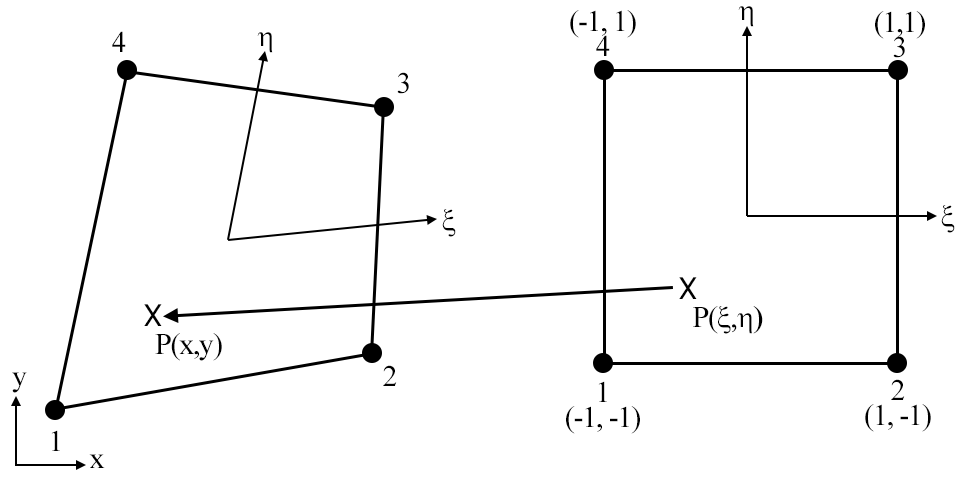
\includegraphics[width=0.97\linewidth]{figures/coord_trafo}
  	\setlength\unitlength{0.99cm}
  	\begin{picture}(14,6)
  	\thicklines
  	\put(0.4,0.3){\vector(1.5,0){1.5}}
  	\put(0.4,0.3){\vector(0,1.5){1.5}}
  	\put(2,0.2){$\mathbf{x}$}
  	\put(0.3,2){$\mathbf{y}$}
  	
  	\polyline(1,1)(6,2)(6.3,4.5)(2.5,5.3)(1,1)
  	\put(1,1){\circle*{0.2}}
  	\put(6,2){\circle*{0.2}}
  	\put(6.3,4.5){\circle*{0.2}}
  	\put(2.5,5.3){\circle*{0.2}}
  	\polyline(10,1)(13.5,1)(13.5,4.5)(10,4.5)(10,1)
  	\put(10,1){\circle*{0.2}}
  	\put(13.5,1){\circle*{0.2}}
  	\put(13.5,4.5){\circle*{0.2}}
  	\put(10,4.5){\circle*{0.2}}
  	
  	\thinlines
  	\put(11.75,2.75){\vector(2,0){2}}
  	\put(13.8,2.6){$\xi$}
  	\put(11.75,2.75){\vector(0,2){2}} 
  	\put(11.6,4.9){$\eta$}
  	
  	\put(3.95,3.2){\vector(2.7,0.2){2.7}}
  	\put(6.80,3.2){$\xi$}
  	\put(3.95,3.2){\vector(0.7,2.3){0.7}} 
  	\put(4.60,5.6){$\eta$}
  	
  	\put(9.6,0.8){$1$}
  	\put(9.3,0.5){$(-1,-1)$}
  	\put(13.7,0.8){$2$}
  	\put(12.7,0.5){$(1,-1)$}
  	\put(13.75,4.35){$3$}
  	\put(13.1,4.75){$(1,1)$}
  	\put(9.6,4.35){$4$}
  	\put(9.3,4.75){$(-1,1)$}
  	
  	\put(0.9,0.5){$1$}
  	\put(5.9,1.5){$2$}
  	\put(6.5,4.4){$3$}
  	\put(2.1,5.2){$4$}
  	
  	\put(10.75,1.75){$\times P(\xi,\eta)$}
  	\put(2.5,2.25){$\times$}
  	\put(2.3,1.9){$P(x,y)$}
  	\thicklines
  	\put(10.7,1.85){\vector(-7.9,0.55){7.9}}
  	\end{picture}
  	\caption{Coordinate transformation of four node quadrilateral element with physical space on the left side and reference space on the right side}
  	\label{fig:coord_trafo}
  \end{figure}
  
  %- eigenschaften der ansatzfunktion + formfunktionen\\
  Similarly to the triangular element, interpolating the displacement field as well as the element geometry is done by shape functions. They are defined in reference coordinates. The displacement of a point within the element can be expressed by the displacements at the nodes and shape functions $\underline{N}$. Also, the position of that point can be expressed in terms of the (global) nodal positions and shape functions $\underline{\tilde{N}}$. The element is called \textit{isoparametric} if $\underline{N}$ is identical to $\underline{\tilde{N}}$. If $\underline{\tilde{N}}$ is of lower degree than $\underline{N}$, the element is called \textit{subparametric} and \textit{superparametric} if it is the other way around \cite{cook2002concepts}.
  
  %- verschiebungen von uv mit formfunktionen und u darstellen\\
  Every node has two degrees of freedom: A displacement $u$ along the x-axis and a displacement $v$ along the y-axis. To find the shape functions it does not matter which variable to choose, so the following basis function was used for $\phi$ which can either represent $u$ or $v$ \cite{steinke2005finite}:
  \begin{equation}\label{eq:q4basis}
  \phi(\xi,\eta) = a_0 + a_1\xi + a_2\eta + a_3\xi\eta = \begin{pmatrix}
  1&\xi&\eta&\xi\eta
  \end{pmatrix}\begin{pmatrix}
  a_0\\a_1\\a_2\\a_3
  \end{pmatrix} = \vec{x}^T\vec{a}
  \end{equation}
  The interpolation conditions at the nodes are as follows:
  \begin{align}
  \phi(-1,-1) &= \phi_1 \rightarrow \phi_1 = a_0 -a_1 -a_2 +a_3 \nonumber\\
  \phi(1,-1) &= \phi_2 \rightarrow \phi_2 = a_0 +a_1 -a_2 -a_3 \nonumber\\
  \phi(1,1) &= \phi_3 \rightarrow \phi_3 = a_0 +a_1 +a_2 +a_3 \nonumber\\
  \phi(-1,1) &= \phi_4 \rightarrow \phi_4 = a_0 -a_1 +a_2 -a_3
  \end{align}
  or in matrix notation:
  \begin{align}
  \underline{A}\vec{a} &= \vec{\phi} \nonumber\\
  \begin{pmatrix}
  1 &-1&-1& 1\\
  1 & 1&-1&-1\\
  1 & 1& 1& 1\\
  1 &-1& 1&-1
  \end{pmatrix} \begin{pmatrix}
  a_0\\a_1\\a_2\\a_3
  \end{pmatrix} &= \begin{pmatrix}
  \phi_1\\\phi_2\\\phi_3\\\phi_4
  \end{pmatrix}
  \end{align}
  Inversion of $\underline{A}$ yields the coefficients $a_i$:
  \begin{equation}
  \vec{a} = \underline{A}^{-1}\vec{\phi} = \frac{1}{4} \begin{pmatrix}
  1&1&1&1\\
  -1&1&1&-1\\
  -1&-1&1&1\\
  1&-1&1&-1
  \end{pmatrix} \begin{pmatrix}
  \phi_1\\\phi_2\\\phi_3\\\phi_4
  \end{pmatrix}
  \end{equation}
  If the last equation is inserted into \eqref{eq:q4basis} one gets the shape functions $\vec{N}$ for the quadrilateral element:
  \begin{align}
  \phi &= \vec{x}^T\underline{A}^{-1}\vec{\phi} \nonumber\\
    &= \vec{N}^T\vec{\phi} \nonumber\\
    &= \frac{1}{4} \begin{pmatrix}
    1&\xi&\eta&\xi\eta
    \end{pmatrix} \begin{pmatrix}
    1&1&1&1\\
    -1&1&1&-1\\
    -1&-1&1&1\\
    1&-1&1&-1
    \end{pmatrix} \vec{\phi} \nonumber\\
    &= \begin{pmatrix}
    \frac{1}{4}(1-\xi)(1-\eta)&\frac{1}{4}(1+\xi)(1-\eta)&\frac{1}{4}(1+\xi)(1+\eta)&\frac{1}{4}(1-\xi)(1+\eta)
    \end{pmatrix} \vec{\phi}
  \end{align}
  One can evaluate shape function $i$ with the $\xi\eta$-coordinates of node $i$. If it evaluates to 1 while at any other node coordinates it evaluates to zero the shape function is correctly set. Now, the displacements can be expressed as follows:
  \begin{equation}
  \vec{\tilde{u}} = \begin{pmatrix}
  u\\v
  \end{pmatrix} = \underline{N}\vec{u} = \begin{pmatrix}
  N_1&0&N_2&0&N_3&0&N_4&0\\
  0&N_1&0&N_2&0&N_3&0&N_4
  \end{pmatrix} \begin{pmatrix}
  u_1\\v_1\\u_2\\v_2\\u_3\\v_3\\u_4\\v_4
  \end{pmatrix}
  \end{equation}
  with $\underline{N}$ being the matrix containing the shape functions and $\vec{u}$ being the vector of the nodal displacements.
  
  %- jacobi-matrix aufstellen, inverse und determinante nicht so genau (bzw. einfach, weil J eh nur 2x2 ist)\\
  The assembly of the strain-displacement matrix $\underline{B}$ is more complicated with isoparametric elements. Due to the $\xi\eta$-coordinates one cannot easily describe an operator such as $\partial/\partial x$. The first step is to formulate a function $\phi = \phi(\xi,\eta)$. Like in the derivation on the shape functions $\phi$ can represent $u$ or $v$. Derivatives with respect to $\xi$ and $\eta$ are as follows \cite{cook2002concepts}:
  \begin{align}
  \frac{\partial \phi}{\partial \xi} = \frac{\partial \phi}{\partial x} \frac{\partial x}{\partial \xi} + \frac{\partial \phi}{\partial y} \frac{\partial y}{\partial \xi} \nonumber\\
  \frac{\partial \phi}{\partial \eta} = \frac{\partial \phi}{\partial x} \frac{\partial x}{\partial \eta} + \frac{\partial \phi}{\partial y} \frac{\partial y}{\partial \eta}
  \end{align}
  or in matrix notation:
  \begin{equation}\label{eq:q4derivRS=J*derivXY}
  \vec{\tilde{\phi}} = \underline{J} \vec{\phi}
  \end{equation}
  where $\underline{J}$ is the Jacobian matrix
  \begin{equation}
  \underline{J} = \begin{pmatrix}
  \sum N_{i,\xi}x_i & \sum N_{i,\xi}y_i\\
  \sum N_{i,\eta}x_i & \sum N_{i,\eta}y_i
  \end{pmatrix}
  \end{equation}
  and $N_{i,j}$ denotes the derivation of the $i$-th shape function with respect to $j$ and $x_i$ the $i$-th component of the $\vec{x}$ vector. The Jacobian matrix can be written out as follows:
  \begin{align}
  \underline{J} &= \frac{1}{4}\begin{pmatrix}
  -(1-\eta) & (1-\eta) & (1+\eta) & -(1+\eta)\\
  -(1-\xi) & -(1+\xi) & (1+\xi) & (1-\xi)
  \end{pmatrix} \begin{pmatrix}
  x_1 & y_1\\
  x_2 & y_2\\
  x_3 & y_3\\
  x_4 & y_4
  \end{pmatrix} \nonumber\\
  &= \begin{pmatrix}
  (x_{12}+x_{34})\eta - x_{12} + x_{34} & (y_{12} + y_{34})\eta - x_{12} + y_{34}\\
  (x_{12}+x_{34})\xi  - x_{13} - x_{24} & (y_{12} + y_{34})\xi  - y_{13} + y_{24}
  \end{pmatrix}
  \end{align}
  Next, equation \eqref{eq:q4derivRS=J*derivXY} can be rearranged to get the derivatives with respect to $x$ and $y$:
  \begin{equation}
  \vec{\phi} = \underline{J}^{-1}\vec{\tilde{\phi}}
  \end{equation}
  
  %- dehnungs-verschiebungs-beziehung
  With the derivatives calculated, the strain-displacement relation \eqref{eq:displ_strain_relation} can be obtained \cite{cook2002concepts}:
  \begin{align}
  \vec{\varepsilon} &= \begin{pmatrix}
  \frac{\partial u}{\partial x} \\
  \frac{\partial v}{\partial y} \\
  \frac{\partial u}{\partial y} + \frac{\partial v}{\partial x}
  \end{pmatrix} = \underbrace{\begin{pmatrix}
  1&0&0&0\\
  0&0&0&1\\
  0&1&1&0
  \end{pmatrix}} \begin{pmatrix}
  {\partial u}/{\partial x} \\ {\partial u}/{\partial y} \\ {\partial v}/{\partial x} \\ {\partial v}/{\partial y}
  \end{pmatrix} \\
  &\qquad\qquad\qquad\qquad\qquad\,\: \underline{L} \nonumber
  \end{align}
  \begin{align}
  \begin{pmatrix}
  {\partial u}/{\partial x} \\ {\partial u}/{\partial y} \\ {\partial v}/{\partial x} \\ {\partial v}/{\partial y}
  \end{pmatrix} &= \underbrace{\begin{pmatrix}
  j_{11} & j_{12} & 0 & 0\\
  j_{21} & j_{22} & 0 & 0\\
  0 & 0 & j_{11} & j_{12}\\
  0 & 0 & j_{21} & j_{22}
  \end{pmatrix}} \begin{pmatrix}
  {\partial u}/{\partial \xi} \\ {\partial u}/{\partial \eta} \\ {\partial v}/{\partial \xi} \\ {\partial v}/{\partial \eta}
  \end{pmatrix}\\
  &\qquad\qquad\quad\,\: \underline{\hat{J}} \nonumber
  \end{align}
  \begin{align}
  \begin{pmatrix}
  {\partial u}/{\partial \xi} \\ {\partial u}/{\partial \eta} \\ {\partial v}/{\partial \xi} \\ {\partial v}/{\partial \eta}
  \end{pmatrix} &= \underbrace{\begin{pmatrix}
  N_{1,\xi}  & 0 N_{2,\xi}  & 0 & N_{3,\xi}  & 0 & N_{4,\xi}  & 0\\
  N_{1,\eta} & 0 N_{2,\eta} & 0 & N_{3,\eta} & 0 & N_{4,\eta} & 0\\
  0 & N_{1,\xi}  & 0 N_{2,\xi}  & 0 & N_{3,\xi}  & 0 & N_{4,\xi}\\
  0 & N_{1,\eta} & 0 N_{2,\eta} & 0 & N_{3,\eta} & 0 & N_{4,\eta}
  \end{pmatrix}} \begin{pmatrix}
  u_1\\v_1\\u_2\\v_2\\u_3\\v_3\\u_4\\v_4
  \end{pmatrix}\\
  &\qquad\qquad\qquad\qquad\qquad\quad\; \underline{\hat{N}} \nonumber
  \end{align}
  where $j_{i}$ denotes the $i$-th entry in the inverse Jacobian matrix.
  The composition of the previous three equations forms the matrix $\underline{B}$:
  \begin{equation}
  \underline{B} = \underline{L}\,\underline{\hat{J}}\,\underline{\hat{N}}
  \end{equation}
  

  %- stefigkeitsmatrix $K = int_V(B^TDBdV) = t*int_V(B^TDBdA) = t*int_-1^1 int_-1^1(B^TDB|J|dsdr)$ + erwähnen, dass |J| Flächeninhalt angibt (ref finden)
  Together with the functional equation \eqref{eq:t3functional} and the material matrix $\underline{D}$ (eq. \eqref{eq:sigma=D*eps}), the stiffness matrix for the quadrilateral isoparametric element can be written as:
  \begin{equation}
  \underline{K} = \int_V \underline{B}^T \underline{D}\,\underline{B}\, dV = t\int_A \underline{B}^T \underline{D}\,\underline{B}\, dA = t\int_{-1}^{1}\int_{-1}^{1} \underline{B}^T \underline{D}\,\underline{B}\, |\underline{J}| d\xi d\eta
  \end{equation}
  For the Quad-4 element a Gaussian quadrature needs four Gauss integration points to satisfy the above equation \cite{steinke2005finite}. These four points are located at $\xi_i = \pm \frac{\sqrt{3}}{3}$ and $\eta_i = \pm \frac{\sqrt{3}}{3}$ with weight factors $\omega_i = 1$. The equation for the stiffness matrix can then be written in discretized form as follows:
  \begin{equation}
  \underline{K} = t \sum_{i=1}^{2} \sum_{j=1}^{2} \omega_i \omega_j \underline{B}(\xi_i,\eta_j)^T \underline{D}\, \underline{B}(\xi_i,\eta_j) |\underline{J}(\xi_i,\eta_j)|
  \end{equation}
 
 \subsection{Plate Bending Element}\label{sec:Shell-Plate}
  In contrast to the plane element, the load at the plate (bending) elements are applied transversal to the element's mid-surface producing plate bending. It has one deformation degree of freedom and two rotational degrees of freedom. Plate elements are often used to model floors or ceilings. In this section, the plate element is discussed in more detail and two discretizations are described: The three-node triangular plate element and the four-node quadrilateral plate element.  
  
  \subsubsection{Problem Definition}\label{sec:Shell-Plate-ProbDef}
  %\cite{steinke2005finite} ch8.1
  \begin{figure}[htbp] % bild wie bei \ref{sec:MprobDef}
  	\centering
  	%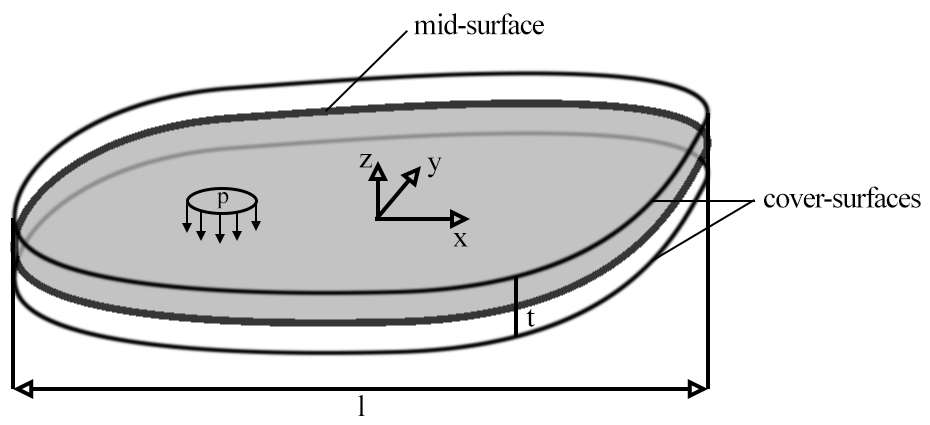
\includegraphics[width=0.9\linewidth]{figures/plate}
  	\setlength\unitlength{1.0cm}
  	\begin{picture}(12,6)
  	\thinlines
  	\put(0,0){\pgfsetfillopacity{1.0}\Curve(0.5,2.5)<0,0.25>(3.5,4.25)<1,0.125>(7.5,4.5)<1,0>(10,2.5)<-1,-1>(6,1)<-0.5,-0.05>(2.5,1)<-0.5,0.125>(0.5,2.5)<0,0.5>}
  	\thicklines
  	{\pgfsetfillopacity{0.8}\color{gray}\Curve*(0.5,3)<0,0.25>(3.5,4.75)<1,0.125>(7.5,5)<1,0>(10,3)<-1,-1>(6,1.5)<-0.5,-0.05>(2.5,1.5)<-0.5,0.125>(0.5,3)<0,0.5>}
  	\put(0,0){\pgfsetfillopacity{1.0}\color{black}\Curve(0.5,3)<0,0.25>(3.5,4.75)<1,0.125>(7.5,5)<1,0>(10,3)<-1,-1>(6,1.5)<-0.5,-0.05>(2.5,1.5)<-0.5,0.125>(0.5,3)<0,0.5>}
    \put(6.6,2.9){$x$}
    \put(5.5,3){\vector(1,0){1}}
    \put(6.1,3.4){$y$}
    \put(5.5,3){\vector(0.5,0.65){0.5}}
    \put(5.4,4.1){$z$}
    \put(5.5,3){\vector(0,1){1}}
  	\thinlines
  	\put(0,0){\pgfsetfillopacity{1.0}\Curve(0.5,3.5)<0,0.25>(3.5,5.25)<1,0.125>(7.5,5.5)<1,0>(10,3.5)<-1,-1>(6,2)<-0.5,-0.05>(2.5,2)<-0.5,0.125>(0.5,3.5)<0,0.5>}
  	\Dline(0.5,3.5)(0.5,0.5){0.1}
  	\Dline(10.37,3.5)(10.37,0.5){0.1}
  	\put(5,0.5){\vector(-4.5,0){4.5}}
  	\put(5,0.5){\vector(5.37,0){5.37}}
  	\put(5.4,0.15){$l$}
  	\Line(2.5,2)(2.5,1)\put(2.43,0.7){$t$}
  	\polyline(10,3.5)(11,3)(10,2.5)\put(11.1,2.9){cover-surfaces}
  	\Line(7.5,5)(9.5,5.5)\put(9.6,5.4){mid-surface}
  	
  	\put(2.5,3){\cbezier(0,0)(0,0.25)(1,0.25)(1,0)}\put(2.5,3){\cbezier(0,0)(0,-0.25)(1,-0.25)(1,0)}\put(2.9,2.9){$p$}
  	\put(2.5,3.5){\vector(0,-0.5){0.5}}\put(3.5,3.5){\vector(0,-0.5){0.5}}\put(3,3.67){\vector(0,-0.5){0.5}}
  	\end{picture}
  	\caption{Schematic drawing of a Kirchhoff plate with its main dimension $l$, thickness $t$ and loading $p$ normal to the mid-surface}
  	\label{fig:plate}
  \end{figure}
  In contrast to a plane, where the load is located planar with respect to the plane, the load is perpendicular to the mid place at a plate. Therefore plate element problems are important for supporting structures of bridges or ceilings and floors in buildings, for example. In Figure \ref{fig:plate} one can see a generalized plate object. It has a main dimension of $l$ and a constant thickness $t$. With the assumption that $t \ll l$, the problem becomes two dimensional and, instead of the whole object, only the middle plane between the two surface areas will be considered. The object has a local coordinate system with its xy-plane the mid plane and its z-axis perpendicular to this plane. The surface areas are located at $z = \pm t/2$. As stated in the beginning, the load is applied in z-direction, i.e. normal to the mid-surface.
  
  % hier wird die kirchhoff-platten-theorie verwendet
  In this work Kirchhoff's theory of thin plates is used. For thick plates or laminated plates, the theory of Reissner-Mindlin is more applicable \cite{werkle1995finite}. The main difference is that with Reissner-Mindlin plates one takes the shear deformations into account. Thus, the normal to the mid-surface remains straight but not necessarily perpendicular to it; instead of a Kirchhoff plate: Here, the normal remains normal to the mid-surface even after deformation.
  
  % voraussetzungen der kirchhoff-platte
  As a short summarize the following conditions must be satisfied for a Kirchhoff plate \cite{steinke2005finite}:
  \begin{itemize}
  	\item The thickness $t$ must be much smaller than the main dimension $l$: $t \ll l$.
  	\item Straight lines normal to the mid-surface remain straight after deformation.
  	\item Straight lines normal to the mid-surface remain normal to the mid-surface after deformation.
  	\item There is only a small amount of deformation $w$, i.e. $w < t$ and it holds $w \ne w(z)$.
  	\item The plate is symmetrical to the mid-surface and changes in thickness must be very small.
  	\item Normal stresses in z-direction $\sigma_{zz}$ will be neglected.
  \end{itemize}
  
  % größen der platte: durchbiegung w + verdrehungen dw/dx bzw. dw/dy
  With \cite{klein2013fem} and \cite{steinke2005finite} the following displacement terms can be formulated:
  \begin{align}
  w &= w(x,y) \\
  u &= -z \frac{\partial w}{\partial x}\\
  v &= -z \frac{\partial w}{\partial y}
  \end{align}
  The deformation $w$ suffices to explain the whole displacement vector. The two derivatives in the equations above describe the torsions around the x- and y-axis.

  % dehnungs-verschiebungs-beziehung
  Similar to the plane element, the Kirchhoff plate element can have a plane strain or plane stress, respectively \cite{steinke2005finite}, i.e. equation \eqref{eq:displ_strain_relation} can be applied here, too:
  \begin{align}
  \vec{\hat{u}} &= \begin{pmatrix}
  u\\v
  \end{pmatrix} = -z \begin{pmatrix}
  \frac{\partial w}{\partial x}\\ \frac{\partial w}{\partial y}
  \end{pmatrix} = -z \nabla w \nonumber\\
  \vec{\varepsilon} &= \underline{L} \vec{\hat{u}} = -z \underline{L} \nabla w = -z \vec{\Delta} w = -z \vec{\kappa} \label{eq:eps=-z*kappa}\\
  \vec{\Delta} &= \underline{L} \nabla = \begin{pmatrix}
  \frac{\partial}{\partial x} & 0\\
  0 & \frac{\partial}{\partial y}\\
  \frac{\partial}{\partial y} & \frac{\partial}{\partial x}
  \end{pmatrix} \begin{pmatrix}
  \frac{\partial}{\partial x} & \frac{\partial}{\partial y}
  \end{pmatrix} = \begin{pmatrix}
  \frac{\partial^2}{\partial x^2}\\
  \frac{\partial^2}{\partial y^2}\\
  2\frac{\partial^2}{\partial x\partial y}
  \end{pmatrix} \nonumber\\
  \vec{\kappa} &= \vec{\Delta}w = \begin{pmatrix}
  \frac{\partial^2w}{\partial x^2}\\
  \frac{\partial^2w}{\partial y^2}\\
  2\frac{\partial^2w}{\partial x\partial y}
  \end{pmatrix} \label{eq:kappa=Delta*w}
  \end{align}
  
  % stoffgleichung (krümmungs-momenten-beziehung) -> führt auf Dp und Querkräfte Qx,Qy
  Referring \cite{klein2013fem} ($\sigma_{zz} = 0, \tau_{xz} = \tau_{yz} = 0$), equation \eqref{eq:stress-strain-relation} can be filled with the above information:
  \begin{align}\label{eq:sigma=-z*D*kappa}
  \vec{\sigma} &= \underline{D} \vec{\varepsilon} = -z \underline{D} \vec{\kappa} \nonumber\\
               &= -\frac{E z}{1-\nu^2} \begin{pmatrix}
               1&\nu&0\\
               \nu&1&0\\
               0&0&\frac{1-\nu}{2}
               \end{pmatrix} \begin{pmatrix}
               \kappa_x\\\kappa_y\\2\kappa_{xy}
               \end{pmatrix}
  \end{align}
  The integration of the stresses $\vec{\sigma}$ over the thickness results in the vector of moments $\vec{M}^T = \left(M_{xx}\ \;M_{yy}\ \;M_{xy}\right)$ \cite{steinke2005finite}:
  \begin{equation}\label{eq:M=-Dp*kappa}
  \vec{M} = \int_{-t/2}^{t/2} z\vec{\sigma} dz = -\int_{-t/2}^{t/2} z^2 \underline{D} \vec{\kappa} dz = -\underline{D} \vec{\kappa} \int_{-t/2}^{t/2} z^2 dz = -\frac{t^3}{12} \underline{D} \vec{\kappa} = -\underline{D}_p \vec{\kappa}
  \end{equation}
  The above equation relates the moments with the curvatures of the plate. The integrals over the transverse stresses $\sigma_{xz}$ and $\sigma_{yz}$ lead to the following shear forces, as described in \cite{steinke2005finite}:
  \begin{align}
  Q_x &= \int_{-t/2}^{t/2}\sigma_{xz} dz = \int_{-t/2}^{t/2} \sigma_{xz}^{\max} \left(1-4\left(\frac{z}{t}\right)^2\right)dz = \frac{2}{3} \sigma_{xz}^{\max} t \nonumber\\
  &= \frac{2}{3} \sigma_{xz}(z=0) t
  \end{align}
  \begin{align}
  Q_y &= \int_{-t/2}^{t/2}\sigma_{yz} dz = \int_{-t/2}^{t/2} \sigma_{yz}^{\max} \left(1-4\left(\frac{z}{t}\right)^2\right)dz = \frac{2}{3} \sigma_{yz}^{\max} t \nonumber\\
  &= \frac{2}{3} \sigma_{yz}(z=0) t
  \end{align}
  The transverse stress is distributed quadratically over the thickness t, i.e. they have their maximum at $z=0$ and vanish at $z = \pm t/2$. The equilibrium of forces in z-direction leads to:
  \begin{equation}\label{eq:dQx+dQy+p=0}
  \frac{\partial Q_x}{\partial x} + \frac{\partial Q_y}{\partial y} + p = 0
  \end{equation}
  with $p$ the load applied perpendicular to the mid-surface. Additionally the equilibrium of moments around the x- and y-axis:\\
  \begin{align}\label{eq:dMxx+dMxy+Qx=0}
  \frac{\partial M_{xx}}{\partial x} + \frac{\partial M_{xy}}{\partial y} + Q_x &= 0 \nonumber\\
  \frac{\partial M_{yy}}{\partial y} + \frac{\partial M_{xy}}{\partial x} + Q_y &= 0
  \end{align}
  % gleichgewichtsbeziehung der platte (p ist flächenlast; näher untersuchen)
  Putting equation \eqref{eq:dMxx+dMxy+Qx=0} into \eqref{eq:dQx+dQy+p=0} results in:
  \begin{equation}\label{eq:Delta^T*M=p}
  \frac{\partial^2 M_{xx}}{\partial x^2} + \frac{\partial^2 M_{yy}}{\partial y^2} + 2\frac{\partial^2 M_{xy}}{\partial x\partial y} = \vec{\Delta}^T \vec{M} = p
  \end{equation}
  Now, one can insert the kinematic equation \eqref{eq:kappa=Delta*w} into equation \eqref{eq:M=-Dp*kappa} and then into the equilibrium relation \eqref{eq:Delta^T*M=p}:
  \begin{align}
  \vec{\kappa} &= \vec{\Delta}w \nonumber\\
  \vec{M} &= -\underline{D}_p \vec{\kappa} = -\underline{D}_p \vec{\Delta} w \nonumber\\
  \vec{\Delta}^T \vec{M} &= -\vec{\Delta}^T \underline{D}_p \vec{\Delta} w = p
  \end{align}
  The last equation leads to the partial differential equation of the plate bending \cite{klein2013fem}:
  \begin{equation}
  \frac{\partial^4 w}{\partial x^4} + \frac{\partial^4 w}{\partial y^4} + 2\frac{\partial^4 w}{\partial x^2 \partial y^2} = -\frac{12(1-\nu^2)}{E t^3} p = \frac{p}{k}
  \end{equation}
  with $k$ denoted as \textit{plate stiffness}.
  
  % auf verschiedene randbedingungen der platte eingehen
  \begin{figure}[htbp] % Bild 8.5 steinke
  	\centering
  	%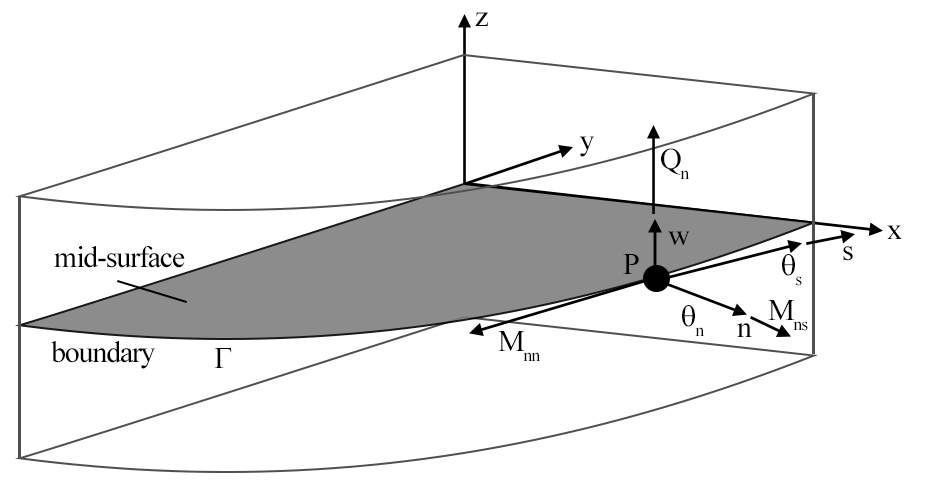
\includegraphics[width=0.97\linewidth]{figures/plate_boundary}
  	\setlength\unitlength{1.0cm}
  	\begin{picture}(13,5.5)
  	\thicklines
  	\put(12.8,3.1){$x$}
  	\put(0,2){\vector(7,1.5){8.5}}
  	\put(8.6,3.8){$y$}
  	\put(7,3.5){\vector(0,2){2}}
  	\put(7.2,5.4){$z$}
  	\put(7,3.5){\vector(5,-0.5){6}}
  	\thinlines
  	\polyline(0,0.5)(0,3.5)(7,5)(12,4.5)(12,1.5)
  	\Dline(7,2)(7,3.5){0.1}
  	\Dline(7,2)(0,0.5){0.1}
  	\Dline(7,2)(12,1.5){0.1}
  	{\pgfsetfillopacity{0.8}\color{gray}\Curve*(0,2)<1,-0.1>(12,3)<7,3>(12,3)<0,0>(7,3.5)<0,0>(0,2)<0,0>}
  	\put(0,0){\pgfsetfillopacity{1.0}\Curve(0,2)<1,-0.1>(12,3)<7,3>}
  	\put(0,0.5){\cbezier(0,0)(1,-0.1)(7,-1)(12,1)}
  	\put(0,3.5){\cbezier(0,0)(1,-0.1)(7,-1)(12,1)}
  	\thicklines
  	\put(10,2.31){\circle*{0.2}}\put(9.65,2.35){$P$}
  	\put(10,2.31){\vector(0,1){1.3}}\put(10.1,2.8){$w$}
  	\put(10,3.66){\vector(0,1){0.7}}\put(10.1,3.65){$Q_n$}
  	\put(10,2.31){\vector(1,0.25){1.5}}\put(11.1,2.25){$\theta_s$}
  	\put(11.6,2.7){\vector(1,0.25){0.75}}\put(12.1,2.55){$s$}
  	\put(10,2.31){\vector(-1,-0.25){1.5}}\put(8.75,1.7){$M_{nn}$}
  	\put(10,2.31){\vector(1,-0.4){1}}\put(10.4,1.75){$n$}
  	\put(11.1,1.85){\vector(1,-0.4){0.5}}\put(11.1,1.45){$\theta_n$}\put(11.3,1.85){$M_{ns}$}
  	\Line(1.4,2.7)(2.3,2.1)\put(0.5,2.8){mid-surface}
  	\put(0.5,1.4){boundary}
  	\put(3,1.35){$\Gamma$}
  	\end{picture}
  	\caption{Part of a plate's boundary with its essential and natural boundary conditions}
  	\label{fig:plate_boundary}
  \end{figure}
  Let $P$ be a point on the continuous boundary of the plate with a local Cartesian coordinate system as described in \cite{steinke2005finite} (see Figure \ref{fig:plate_boundary}): The $n$ coordinate is perpendicular to the boundary surface, the $s$ axis tangential to it. The third axis equals the global z-axis of the plate. There are three essential and three natural boundary conditions defined for $P$: The displacement $w$, the drills $\theta_n = \partial w/\partial s, \theta_s = -\partial w/\partial n$, the shear force $Q_n$ and the moments $M_{ns}$ and $M_{nn}$. Since this leads to an inconsistency with the differential equation above, \cite{steinke2005finite} stated that Kirchhoff introduced new forces:
  \begin{equation}
  V_n = Q_n - \frac{\partial M_{ns}}{\partial s}
  \end{equation}
  With them, only the four conditions for $w, \theta_s, V_n$ and $M_{nn}$ occur.
  The plate can be mounted in different ways:
  \begin{itemize}
  	\item clamped: $w = 0, \theta_s = -\partial w/\partial n = 0$
  	\item simple supported: $w = 0, M_{nn} = 0$
  	\item symmetrical edge: $\theta_s = -\partial w/\partial n = 0, V_n = 0$
  \end{itemize}

  % funktional der platte
  The plate's functional as described in \cite{steinke2005finite} is given below:
  \begin{equation}
  \frac{1}{2} \int_V \vec{\varepsilon}^T \vec{\sigma}\, d\:\!V
  \end{equation}
  One can insert equation \eqref{eq:eps=-z*kappa} and \eqref{eq:sigma=-z*D*kappa} into the functional:
  \begin{equation}
  \frac{1}{2} \int_V \vec{\varepsilon}^T \vec{\sigma}\, d\:\!V = \frac{1}{2}\int_V \vec{\kappa}^T \underline{D} \vec{\kappa} z^2\, d\!V = \frac{1}{2} \int_A \vec{\kappa}^T \underline{D}_p \vec{\kappa}\, d\!A
  \end{equation}
  Together with the potential of the external forces the overall potential of the Kirchhoff plate is:
  \begin{equation}\label{eq:plateFunctional}
  \Pi = \frac{1}{2}\int_A \vec{\kappa}^T \underline{D}_p \vec{\kappa}\, dA
  - \int_A p\ w\, d\!A
  - \int_{\Gamma}\left(V_n w - M_{nn} \theta_s\right)\,d\:\!\Gamma
  \end{equation}
  
  % forderungen an plattenelement
  Klein \cite{klein2013fem} states that for the plate element discretization additional conditions must be satisfied. They are: The bending $w(x,y)$ as well as the normal derivative $\partial w/\partial n$ at the element's boundary must be continuous to the neighboring elements. This would be the case if the bending and the normal derivative are explicitly determined by the nodal parameters at the border. Further, Klein lists requirements for a plate element ansatz:
  \begin{itemize}
  	\item Totality of the displacement approach in order to guarantee good convergence.
  	\item The terms $1, x, y, x^2, xy, y^2$ should be included to get variable strains, curvatures and rigid body motion.
  \end{itemize}
  Steinke \cite{steinke2005finite} expands the requirements as follows:
  \begin{itemize}
  	\item Compatibility of the displacement variable at the element's boundary (conformity condition): If the steadiness of the deformation $w$ and its first derivatives is not satisfied the bending surface between two elements can have a sharp bend at which the elements are overlapping at one side and diverge on the opposite side. If such a behavior is shown, the element is called \textit{non-conforming}.
  	\item Rigid body motions must not create strains and stresses in the element. This requires a constant term in the basis function for the translative part of the motion and a linear term for the rotatory.
  	\item The basis function must provide constant plain strain and plain stress: If the element converges in its size until it becomes a point, a constant state of bending must be describable in this situation. Since the bending is described as second order derivatives of $w$, the basis function must include quadratic terms.
  \end{itemize}
  The following sections show details of two discretizations of plate elements: A triangular element with three nodes and a quadrilateral element with four nodes.
  
  \subsubsection{Tri-3 Plate Element}\label{sec:Shell-Plate-Tri}
  There exist many different types of triangular plate elements, for example Batoz et al. \cite{batoz1980study}, Tocher \cite{tocher1963analysis} or Specht \cite{specht1988modified}. The three node triangular element from \cite{tocher1963analysis} has three degrees of freedom (d.o.f) ($w, \theta_x, \theta_y$) per node. His basis function was a complete cubic polynomial. The term $xy$ was left out, because the polynomial has one coefficient more than the element has d.o.f. This leads to the problem that no constant state of bending can be described (non-conforming element) and this leads to wrong results at convergence \cite{steinke2005finite}. Therefore, Steinke challenges the practical use of this element.
  A possible way to use a complete cubic polynomial would be to add another node in the center of mass of the triangle and assign the only degree of freedom $w$ to it \cite{steinke2005finite}. But the problem of non-conformity persist, as the nodal twists don't suffice to describe the twists along the element's edges, which are quadric. Here, additional nodes on the edges would be needed.
  To get a conforming element one can choose a basis function with a complete polynomial of fifth order. It has 21 coefficients and d.o.f. They are distributed as follows: Every node has six d.o.f $(w, \partial w/\partial x, \partial w/\partial y, \partial^2 w/\partial x^2, \partial^2 w/\partial y^2, \partial^2 w/\partial x\partial y)$ and the mid node of every edge gets the degree of freedom $\partial w/\partial n$. A conform element with continuous twists at its edges follows from that. But the 21 d.o.f. per element leads to high computational effort and second order derivatives at the boundaries are needed. Hence, Steinke advices against using it in practice \cite{steinke2005finite}.
  
  % ansatzfunktion nach specht\\
  In this work an element from Specht \cite{specht1988modified} was implemented which is also described in \cite{steinke2005finite}. It has three nodes and also three d.o.f. per node: The deformation $w$ and the two twists $\theta_x$ and $\theta_y$. The basis function for the deformation $w$ is as follows:
  \begin{align}
  w = &a_0 L_1 + a_1 L_2 + a_2 L_3 + a_3 L_1L_2 + a_4 L_2L_3 + a_5 L_3L_1 \nonumber\\
    & + a_6\left(L_2L_1^2 + \frac{1}{2}L_1L_2L_3 \left(3(1-\mu_3)L_1 - (1+3\mu_3)L_2 + (1+3\mu_3)L_3\right)\right) \nonumber\\
    & + a_7\left(L_3L_2^2 + \frac{1}{2}L_1L_2L_3 \left(3(1-\mu_1)L_2 - (1+3\mu_1)L_3 + (1+3\mu_1)L_1\right)\right) \nonumber\\
    & + a_8\left(L_1L_3^2 + \frac{1}{2}L_1L_2L_3 \left(3(1-\mu_2)L_3 - (1+3\mu_2)L_1 + (1+3\mu_2)L_2\right)\right)
  \end{align}
  with
  \begin{align}
  \mu_1 &= \frac{S_{21} - S_{31}}{S_{32}} \nonumber\\
  \mu_2 &= \frac{S_{32} - S_{21}}{S_{31}} \nonumber\\
  \mu_3 &= \frac{S_{31} - S_{32}}{S_{21}} \\
  S_{32} &= x_{32}^2 + y_{32}^2 \nonumber\\
  S_{31} &= x_{31}^2 + y_{31}^2 \nonumber\\
  S_{21} &= x_{21}^2 + y_{21}^2
  \end{align}
  $S_{ij}$ denoted the square of the length of the edge between node $i$ and $j$.
  This can be written is vector form:
  \begin{align}\label{eq:platet3w=x*a}
  w &= \vec{x}^T \vec{a} \nonumber\\
  \vec{x} &= \begin{pmatrix}
  L_1 \\ L_2 \\ L_3 \\ L_1L_2 \\ L_2L_3 \\ L_3L_1\\
  \left(L_2L_1^2+\frac{1}{2}L_1L_2L_3\left(3(1-\mu_3)L_1-(1+3\mu_3)L_2+(1+3\mu_3)L_3\right)\right)\\
  \left(L_3L_2^2+\frac{1}{2}L_1L_2L_3\left(3(1-\mu_1)L_2-(1+3\mu_1)L_3+(1+3\mu_1)L_1\right)\right)\\
  \left(L_1L_3^2+\frac{1}{2}L_1L_2L_3\left(3(1-\mu_2)L_3-(1+3\mu_2)L_1+(1+3\mu_2)L_2\right)\right)
  \end{pmatrix} \nonumber\\
  \vec{a}^T &= \begin{pmatrix}
  a_0 & a_1 & a_2 & a_3 & a_4 & a_5 & a_6 & a_7 & a_8
  \end{pmatrix}
  \end{align}
  
  % interpolationsbedingungen
  The twists $\theta_x$ and $\theta_y$ are to be described in Cartesian coordinates. They must be transformed into triangular coordinates with the help of equation \eqref{eq:t3NablaTilde}:
  \begin{equation}
  \vec{\theta} = \begin{pmatrix}
  \theta_x\\\theta_y
  \end{pmatrix} = \begin{pmatrix}
  0 & 1 \\ -1 & 0
  \end{pmatrix} \nabla w = \begin{pmatrix}
  0 & 1 \\ -1 & 0
  \end{pmatrix} \underline{J}^{-1} \tilde{\nabla} \vec{x}^T \vec{a} = \underline{G} \vec{a}
  \end{equation}
  with $\underline{J}^{-1}$ the inverse Jacobian matrix and $\tilde{\nabla}$ the nabla operator in triangular coordinates. The matrix $\underline{G}$:
  \begin{equation}
  \underline{G} = \frac{1}{2 A_\triangle} \begin{pmatrix}
  x_{32} & x_{13} \\ y_{32} & y_{13}
  \end{pmatrix} \begin{pmatrix}
  \frac{\partial x_1}{\partial L_1} & \frac{\partial x_2}{\partial L_1} & \cdots & \frac{\partial x_9}{\partial L_1} \\
  \frac{\partial x_1}{\partial L_2} & \frac{\partial x_2}{\partial L_2} & \cdots & \frac{\partial x_9}{\partial L_2}
  \end{pmatrix}
  \end{equation}
  Next, the interpolation conditions at the three nodes for the three unknowns can be set (cf. Figure \ref{fig:tri_coords}). Following the notation of \cite{steinke2005finite}:
  \begin{align}
  \underbrace{\begin{pmatrix}
  	\vec{x}^T(1,0)\\G_1(1,0)\\G_2(1,0)\\
  	\vec{x}^T(0,1)\\G_1(0,1)\\G_2(0,1)\\
  	\vec{x}^T(0,0)\\G_1(0,0)\\G_2(0,0)
  	\end{pmatrix}} \vec{a} &= \underbrace{\begin{pmatrix}
  	w_1\\\theta_{x_1}\\\theta_{y_1}\\
  	w_2\\\theta_{x_2}\\\theta_{y_2}\\
  	w_3\\\theta_{x_3}\\\theta_{y_3}
  	\end{pmatrix}}\\
  \underline{A}\qquad\quad &\qquad\ \vec{w}
  \end{align}
  where $\underline{G}_i$ is the $i$-th row of matrix $\underline{G}$.
  The unknown coefficients $a_i$ can be computed by inverting the matrix $\underline{A}$: $\vec{a} = \underline{A}^{-1} \vec{w}$:
  \begin{equation}
  \underline{A}^{-1} = \begin{pmatrix}
  1& 0& 0& 0& 0& 0& 0& 0& 0\\
  0& 0& 0& 1& 0& 0& 0& 0& 0\\
  0& 0& 0& 0& 0& 0& 1& 0& 0\\
  -1& 0& 0& 1& y_{12}& x_{21}& 0& 0& 0\\
  0& 0& 0& -1& 0& 0& 1& y_{23}& x_{32}\\
  1& y_{31}& x_{13}& 0& 0& 0& -1& 0& 0\\
  2& y_{21}& x_{12}& -2& y_{21}& x_{12}& 0& 0& 0\\
  0& 0& 0& 2& y_{32}& x_{23}& -2& y_{32}& x_{23}\\
  -2& y_{13}& x_{31}& 0& 0& 0& 2& y_{13}& x_{31}
  \end{pmatrix}
  \end{equation}
  where $x_{ij}$ and $y_{ij}$ denotes the differences of the node's coordinates $x_i-x_j$ and $y_i-y_j$.
  Now, the coefficients can be inserted into equation \eqref{eq:platet3w=x*a}:
  \begin{equation}\label{eq:w=NT*vecw}
  w = \vec{x}^T \vec{a} = \vec{x}^T \underline{A}^{-1} \vec{w} = \vec{N}^T \vec{w}
  \end{equation}
  The vector $\vec{N}$ containing the shape functions $N_i$ can then be calculated as follows:
  \begin{equation}
  \vec{N} = \left(\underline{A}^{-1}\right)^T \vec{x}
  \end{equation}
  
  % entwicklung der formfunktionen\\
  Since the shape functions follow a pattern, due to the regular order in the matrix $\underline{A}^{-1}$, one can summarize the nine shape functions into three groups; one for every node:
  \begin{align}
  N_i &= \begin{cases}
  \chi_i - \chi_{i+3} + \chi_{k+3} + 2\left(\chi_{i+6} - \chi_{k+6}\right) & \text{for d.o.f. } w\\
  -y_{ki}\left(\chi_{k+6} - \chi_{k+3}\right) + y_{ji} \chi_{i+6} & \text{for d.o.f. } \theta_x\\
  x_{ki}\left(\chi_{k+6} - \chi_{k+3}\right) - x_{ji} \chi_{i+6} & \text{for d.o.f. } \theta_y
  \end{cases}
  \end{align}
  The variables $\chi_i$ denotes the $i$-th component of the vector $\vec{x}$, the indexes $i,j,k$ under $\chi$ are cyclic permutations of $1,2,3$. $x_{ij}$ and $y_{ij}$ denote the coordinate differences $x_i - x_j$ and $y_i - y_j$. The index under $N$ is incremented in such a way, that $N_1, N_4, N_7$ describes the d.o.f. $w$, $N_2, N_5, N_8$ describes the d.o.f. $\theta_x$ and $N_3, N_6, N_9$ describes the d.o.f. $\theta_y$.
  Similar to the plane elements, one can check the correctness of the shape functions by evaluating them at the triangular coordinates of the three triangle's nodes. For example, shape function $N_7$ will evaluate to 1 for the coordinates $(L_1 = 0, L_2 = 0)$ (node 3) and will be zero for $(L_1 = 1, L_2 = 0)$ (node 1) and $(L_1 = 0, L_2 = 1)$ (node 2).
  
  % krümmungs-verschiebungs-beziehung\\
  The displacement-strain relation \eqref{eq:eps=-z*kappa} introduced for the plate element contains an operator living in the Cartesian space. It has to be converted into triangular coordinates. With equation \eqref{eq:nabla=invJ*nabla-tilde} ($\nabla = \underline{J}^{-1}\tilde{\nabla}$) one can describe a second order derivative operator $\Delta$:
  \begin{align}
  \Delta &= \nabla \nabla^T = \underline{J}^{-1}\tilde{\nabla}\left(\underline{J}^{-1}\tilde{\nabla}\right)^T = \underline{J}^{-1} \tilde{\nabla} \tilde{\nabla}^T \left(\underline{J}^{-1}\right)^T = \underline{J}^{-1} \tilde{\Delta} \left(\underline{J}^{-1}\right)^T\\
  \Delta &= \begin{pmatrix}
  \frac{\partial^2}{\partial x^2} & \frac{\partial^2}{\partial x \partial y}\\
  \frac{\partial^2}{\partial y \partial x} & \frac{\partial^2}{\partial y^2}
  \end{pmatrix} \rightarrow \vec{\Delta} = \begin{pmatrix}
  \frac{\partial^2}{\partial x^2} \\
  \frac{\partial^2}{\partial y^2} \\
  2\frac{\partial^2}{\partial x \partial y}
  \end{pmatrix} \nonumber\\
  \vec{\Delta} &= \frac{1}{4 A_\triangle^2} \begin{pmatrix}
  y_{32}^2 & y_{31}^2 & y_{23} y_{31}\\
  x_{32}^2 & x_{31}^2 & x_{13} x_{32}\\
  2 x_{32} y_{23} & 2 x_{13} y_{31} & x_{32} y_{31} + x_{31} y_{32}
  \end{pmatrix} \begin{pmatrix}
  \frac{\partial^2}{\partial L_1^2} \\
  \frac{\partial^2}{\partial L_2^2} \\
  2\frac{\partial^2}{\partial L_1 \partial L_2}
  \end{pmatrix} \nonumber\\
  \vec{\Delta} &= \underline{Y} \vec{\tilde{\Delta}}
  \end{align}
  Next, equation \eqref{eq:eps=-z*kappa} can be rewritten for triangular coordinates:
  \begin{equation}
  \vec{\varepsilon} = -z \vec{\Delta} w = -z \underline{Y} \vec{\tilde{\Delta}} w = -z \vec{\kappa}
  \end{equation}
  And additionally, with the help of equation \eqref{eq:w=NT*vecw}, this yields a new version of equation \eqref{eq:kappa=Delta*w}:
  \begin{equation}\label{eq:kappa=YBw}
  \vec{\kappa} = \vec{\Delta} w = \underline{Y} \vec{\tilde{\Delta}} \vec{N}^T \vec{w} = \underline{Y}\:\underline{\tilde{B}} \vec{w} = \underline{B} \vec{w}
  \end{equation}
  \begin{equation}
  \underline{\tilde{B}} = \vec{\tilde{\Delta}} \vec{N}^T = \begin{pmatrix}
  \frac{\partial^2 N_1}{\partial L_1^2} & \frac{\partial^2 N_2}{\partial L_1^2} & \cdots & \frac{\partial^2 N_9}{\partial L_1^2}\\
  \frac{\partial^2 N_1}{\partial L_2^2} & \frac{\partial^2 N_2}{\partial L_2^2} & \cdots & \frac{\partial^2 N_9}{\partial L_2^2}\\
  2\,\frac{\partial^2 N_1}{\partial L_1 \partial L_2} & 2\,\frac{\partial^2 N_2}{\partial L_1 \partial L_2} & \cdots & 2\,\frac{\partial^2 N_9}{\partial L_1 \partial L_2}
  \end{pmatrix}
  \end{equation}
  
  % steifigkeitsmatrix
  With the help of equation \eqref{eq:kappa=YBw}, the first term (denoted as $\Pi_1$) of the plate element's functional \eqref{eq:plateFunctional} can be written out:
  \begin{align}\label{eq:t3_pi1=0.5wTKw}
  \Pi_1 &= \frac{1}{2} \int_A \vec{\kappa}^T \underline{D}_p \vec{\kappa}\ d\!A \nonumber\\
        &= \frac{1}{2} \vec{w}^T \int_A \underline{B}^T \underline{D}_p \underline{B}\ d\!A \vec{w} \nonumber\\
        &= \frac{1}{2} \vec{w}^T \underline{K} \vec{w}
  \end{align}
  where $\underline{K}$ describes the stiffness matrix for the three node triangular plate element. The stiffness matrix must be integrated in triangular coordinates. This will be done by a Gaussian quadrature with the Gauss points located at: $(L_{1_1} = 1/6, L_{2_1} = 1/6), (L_{1_2} = 2/3, L_{2_2} = 1/6), (L_{1_3} = 1/6, L_{2_3} = 2/3)$ and weights $\omega_i = 1/6$ for all three points. For an exact integration one would accumulate four sampling points, but \cite{steinke2005finite} states that this leads to an element, that is too stiff; with only three samplings a more natural element results.
  \begin{equation}
  \underline{K} = 2 A_\triangle \sum_{i=1}^{3} \omega_i \underline{B}^T(L_{1_i}, L_{2_i}) \underline{D}_p \underline{B}(L_{1_i}, L_{2_i})
  \end{equation}
  The plate's functional \eqref{eq:plateFunctional} has two more terms including the surface load $p$ and edge loads $V_n$. These two can now be written as follows (see also \cite{steinke2005finite}):
  \begin{equation}
  \int_A p\ w\ d\!A = \vec{w}^T \vec{F}_p = \vec{w}^T p \int_A \vec{N}\ d\!A = 2 \vec{w}^T A_\triangle p \int_{0}^{1}\left(\int_{0}^{1-L_1} \vec{N}\ d\,\!L_2\right)\ d\,\!L_1
  \end{equation}
  where $\vec{F}_p$ is a $1\!\times\!9$ vector containing forces and moments emerging from the surface load $p$.
  As an example, an edge load $V_n$ is applied to edge $S_{13}$. This can be described as follows \cite{steinke2005finite}:
  \begin{equation}
  \int_{\Gamma_V} V_n\:w\ d\,\!\Gamma = \int_{\Gamma_V} V_n \vec{w}^T \vec{N}(L_2 = 0)\ d\,\!\Gamma
  \end{equation}
  with $d\,\!\Gamma = S_{13} d\,\!L_1$. With $V_n$ being constant all over the edge:
  \begin{equation}
  \int_{\Gamma_V} V_n \vec{w}^T \vec{N}(L_2 = 0)\ d\,\!\Gamma = \vec{w}^T S_{13} V_n \int_{0}^{1} \vec{N}\ d\,\!L_1 = \vec{w}^T \vec{F}_v
  \end{equation}
  The edge load applies forces and moments contained in $\vec{F}_v$ to the nodes forming that edge. The above equation can be applied to every other edge.
  
  \subsubsection{Quad-4 Plate Element}\label{sec:Shell-Plate-Quad}
  % mathematical derivation of four node quadrilateral plane element
  % see Zienkiewicz \cite{zienkiewicz2000finite} page 174-177,219-222 \cite{batoz1982evaluation page 1658-1662}
  % formulierung als DKQ element
  The Quad-4 element implemented in this work is the so-called Discrete Kirchhoff Quadrilateral (DKQ) element, introduced by Batoz et al. \cite{batoz1982evaluation}. It is a four-node, 12 degrees-of-freedom quadrilateral element for thin plates. It is based on a generalization of the Discrete Kirchhoff Triangular (DKT) element which is a three-node, 9 d.o.f. triangular element. Like the triangular element of the previous section, all the DKQ elements nodes have three degrees of freedom: The displacement $w$ and the rotations $\theta_x$ and $\theta_y$ around the element's local $x$- and $y$-axis. Figure \ref{fig:dkq} shows an example of such an element.
  \begin{figure}[htbp] % Bild 1 batoz
  	\centering
  	%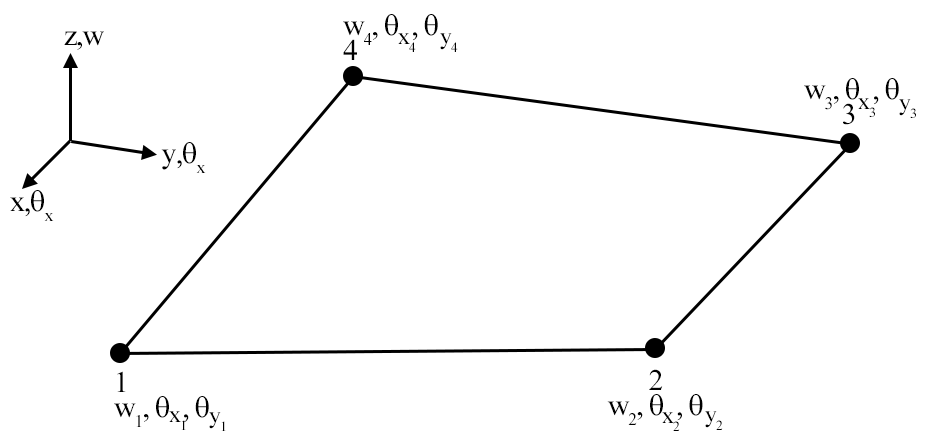
\includegraphics[width=0.97\linewidth]{figures/dkq}
  	\setlength\unitlength{1.0cm}
  	\begin{picture}(12.5,7)
  	\thicklines  
  	\put(1.5,4.5){\vector(0,1){1}}
  	\put(1.2,5.6){$z,w$}
  	\put(1.5,4.5){\vector(1,-0.2){1}}
  	\put(2.6,4.2){$y,\theta_y$}
  	\put(1.5,4.5){\vector(-0.5,-0.5){0.7}}
  	\put(0.6,3.5){$x,\theta_x$}
  	
  	\thinlines
  	\polyline(2.5,1.5)(8.5,1.6)(11.5,5)(5,6)(2.5,1.5)
  	\put(2.5,1.5){\circle*{0.25}}
  	\put(1.7,1.0){$w_1,\theta_{x_1},\theta_{y_1}$}
  	\put(8.5,1.6){\circle*{0.25}}
  	\put(7.8,1.1){$w_2,\theta_{x_2},\theta_{y_2}$}
  	\put(11.5,5){\circle*{0.25}}
  	\put(11.0,5.3){$w_3,\theta_{x_3},\theta_{y_3}$}
  	\put(5,6){\circle*{0.25}}
  	\put(4.2,6.3){$w_4,\theta_{x_4},\theta_{y_4}$}
  	\end{picture}
  	\caption{4-node quadrilateral plate element DKQ with 12 degrees-of-freedom, three per node.}
  	\label{fig:dkq}
  \end{figure}
  

  % dkq basiert auf diskretisierung der stress-energie, unter vernachlässigung der transverse shear strain energy (gl.(1) s.4)
  The formulation of the DKQ element by Batoz et al. \cite{batoz1982evaluation} uses the discrete Kirchhoff technique. It is based on the discretization of the strain energy and neglects the transverse shear energy. This results in the following functional:
  \begin{equation}
  \Pi = \frac{1}{2} \int_A \vec{\kappa}^T \underline{D}_p \vec{\kappa}\ d\!A
  \end{equation}
  where $\underline{D}_p$ is the material matrix as defined previously (equation \eqref{eq:M=-Dp*kappa}) and $\vec{\kappa}$ denotes:
  \begin{equation}
  \vec{\kappa} = \begin{pmatrix}
  \frac{\partial \beta_x}{\partial x}\\
  \frac{\partial \beta y}{\partial y}\\
  \frac{\partial \beta_x}{\partial y} + \frac{\partial \beta_y}{\partial x}
  \end{pmatrix}
  \end{equation}
  $\beta_i$ is the rotation of the normal to the undeformed mid-surface in $x$-$z$-plane and $y$-$z$-plane, respectively. For $\Pi$ only $C^0$ continuity is required \cite{batoz1982evaluation}. Further, Batoz et al. states that $\beta_x$ and $\beta_y$ must be related to $w$ in such a way, that the final element satisfies the following requirements:
  \begin{itemize}
  	\item The nodal variables must be $w$, $\theta_x$ and $\theta_y$ with respect to $x$ and $y$ at the four element's nodes ($\theta_x = \partial w/\partial y, \theta_y=-\partial w/\partial x$)
  	\item The Kirchhoff boundary conditions must be satisfied.
  \end{itemize}
      
  % krümmungsvektor, Db angeben 
  % considerations für dkq formulierung
  Two incomplete cubic polynomial expressions define $\beta_x$ and $\beta_y$:
  \begin{align}
  \beta_x &= \sum_{i=1}^{8} N_i \beta_{x_i}\\
  \beta_y &= \sum_{i=1}^{8} N_i \beta_{y_i}
  \end{align}
  $N_i(\xi,\eta)$ are here the shape functions with isoparametric coordinates $\xi$ and $\eta$. They are the same as of the ``eight-node Serendipity'' element, described for example in \cite{zienkiewicz2000finite}, or \cite{braess2007finite} and seen in Figure \ref{fig:serendipity}. The shape functions of this element are achieved by products of linear Lagrangian polynomials of the form $\frac{1}{4}(\xi+1)(\eta+1)$. For the eight node element the following shape functions result:
  \begin{align}
  N_1(\xi, \eta) &= \frac{1}{4}(1-\xi)(1-\eta)(-\xi-\eta-1) \nonumber\\
  N_2(\xi, \eta) &= \frac{1}{4}(1+\xi)(1-\eta)(\xi-\eta-1) \nonumber\\
  N_3(\xi, \eta) &= \frac{1}{4}(1+\xi)(1+\eta)(\xi+\eta-1) \nonumber\\
  N_4(\xi, \eta) &= \frac{1}{4}(1-\xi)(1+\eta)(-\xi+\eta-1) \nonumber\\
  N_5(\xi, \eta) &= \frac{1}{2}(1-\xi^2)(1-\eta) \nonumber\\
  N_6(\xi, \eta) &= \frac{1}{2}(1+\xi)(1-\eta^2) \nonumber\\
  N_7(\xi, \eta) &= \frac{1}{2}(1-\xi^2)(1+\eta) \nonumber\\
  N_8(\xi, \eta) &= \frac{1}{2}(1-\xi)(1-\eta^2) \nonumber
  \end{align}
  \begin{figure}[htbp] % Bild 8.9 (a) \cite{zienkiewicz2000finite}
  	\centering
  	%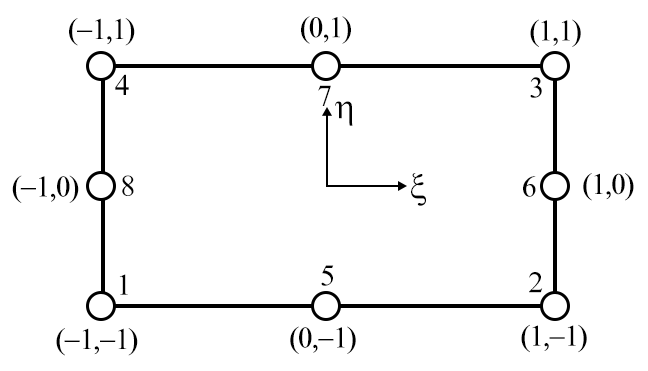
\includegraphics[width=0.97\linewidth]{figures/serendipity}
  	\setlength\unitlength{1.5cm}
  	\begin{picture}(8,5)
  	\thicklines  
  	\polyline(1.5,0.75)(1.5,4.25)(7,4.25)(7,0.75)(1.5,0.75)
  	\put(1.5,0.75){\circle*{0.25}}
  	\put(1.5,4.25){\circle*{0.25}}
  	\put(7,4.25){\circle*{0.25}}
  	\put(7,0.75){\circle*{0.25}}
  	\put(4.25,0.75){\circle*{0.25}}
  	\put(4.25,4.25){\circle*{0.25}}
  	\put(1.5,2.5){\circle*{0.25}}
  	\put(7,2.5){\circle*{0.25}}
  	
  	\thinlines
  	\put(4.25,2.5){\vector(1,0){1.25}}
  	\put(4.25,2.5){\vector(0,1){1.25}}
  	\put(5.3,2.2){$\xi$}
  	\put(4.4,3.5){$\eta$}
  	\put(1.1,4.5){$(-1,1)$}   \put(4.0,4.5){$(0,1)$}   \put(6.7,4.5){$(1,1)$}
  	\put(0.6,2.45){$(-1,0)$}                            \put(7.3,2.45){$(1,0)$}
  	\put(1.1,0.3){$(-1,-1)$}  \put(3.9,0.3){$(0,-1)$}  \put(6.7,0.3){$(1,-1)$}
  	
  	\put(1.7,3.9){$4$}  \put(4.2,3.9){$7$}  \put(6.6,3.9){$3$}
  	\put(1.7,2.4){$8$}                       \put(6.6,2.4){$6$}
  	\put(1.7,0.9){$1$}  \put(4.2,0.9){$5$}  \put(6.6,0.9){$2$}
  	\end{picture}
  	\caption{Eight-node quadrilateral element (``Seredipity''-element) with local $\xi,\eta$-coordinates.}
  	\label{fig:serendipity}
  \end{figure}
  $\beta_{x_i}$ and $\beta_{y_i}$ are transitory nodal variables at the four nodes and mid-sides of the element.
  Next, Batoz et al. described the Kirchhoff assumptions at the corner nodes (cf. Figure \ref{fig:serendipity} for the following):
  \begin{align}
  \begin{pmatrix}
  \beta_{x_i} + \partial w/\partial x_i \\
  \beta_{y_i} + \partial w/\partial y_i
  \end{pmatrix} = \begin{pmatrix}
  0\\0
  \end{pmatrix},\qquad i = 1,2,3,4
  \end{align}
  and at the mid-nodes:
  \begin{align}
  \beta_{s_k} + \partial w/\partial s_k = 0,\qquad k = 5,6,7,8
  \end{align}
  where $s$ denotes the coordinate along the element boundary and $\partial w/\partial s_k$ is the derivative of the displacement $w$ with respect to the mid-node $k$:
  \begin{equation}
  \frac{\partial w}{\partial s_k} = -\frac{3}{2 l_{ij}}(w_i-w_j) - \frac{1}{4}\left(\frac{\partial w}{\partial s_i} + \frac{\partial w}{\partial s_j}\right)
  \end{equation}
  with $k = 5,6,7,8$ being the mid-node of side $ij = 12, 23, 34, 41$ and $l_{ij}$ denotes the length of side $ij$.
  $\beta_n$ varies linearly along the sides:
  \begin{equation}
  \beta_{n_k} = \frac{1}{2}\left(\beta_{n_i} + \beta_{n_j}\right) = -\frac{1}{2} \left(\frac{\partial w}{\partial n_i} + \frac{\partial w}{\partial n_j}\right)
  \end{equation}
  with $k$ same as before.
  % formfunktionen, koeffizienten
  $\beta_x$ and $\beta_y$ can be rewritten as follows:
  \begin{align}
  \beta_x &= \vec{H^x(\xi,\eta)}^T \vec{w}\\
  \beta_y &= \vec{H^y(\xi,\eta)}^T \vec{w}\\
  \vec{w}^T &= \begin{pmatrix}
  w_1&\theta_{x_1}&\theta_{y_1}&w_2&\theta_{x_2}&\theta_{y_2}&w_3&\theta_{x_3}&\theta_{y_3}
  \end{pmatrix} \nonumber
  \end{align}
  with
  \begin{align}
  \vec{H^x}^T &= \begin{pmatrix}
  H_1^x & \dots & H_{12}^x
  \end{pmatrix} \nonumber\\
  H_{\left[1,4,7,10\right]}^x &= \frac{3}{2}\left(a_{\left[5,6,7,8\right]} N_{\left[5,6,7,8\right]} - a_{\left[8,5,6,7\right]} N_{\left[8,5,6,7\right]}\right) \nonumber\\
  H_{\left[2,5,8,11\right]}^x &= b_{\left[5,6,7,8\right]} N_{\left[5,6,7,8\right]} + b_{\left[8,5,6,7\right]} N_{\left[8,5,6,7\right]} \nonumber\\
  H_{\left[3,6,9,12\right]}^x &= N_{\left[1,2,3,4\right]} - c_{\left[5,6,7,8\right]} N_{\left[5,6,7,8\right]} - c_{\left[8,5,6,7\right]} N_{\left[8,5,6,7\right]} \nonumber\\
  \vec{H^y}^T &= \begin{pmatrix}
  H_1^y & \dots & H_{12}^y
  \end{pmatrix} \nonumber\\
  H_{\left[1,4,7,10\right]}^y &= \frac{3}{2}\left(d_{\left[5,6,7,8\right]} N_{\left[5,6,7,8\right]} - d_{\left[8,5,6,7\right]} N_{\left[8,5,6,7\right]}\right) \nonumber\\
  H_{\left[2,5,8,11\right]}^y &= -N_{\left[1,2,3,4\right]} + e_{\left[5,6,7,8\right]} N_{\left[5,6,7,8\right]} + e_{\left[8,5,6,7\right]} N_{\left[8,5,6,7\right]} \nonumber\\
  H_{\left[3,6,9,12\right]}^y &= -b_{\left[5,6,7,8\right]} N_{\left[5,6,7,8\right]} - b_{\left[8,5,6,7\right]} N_{\left[8,5,6,7\right]} \nonumber
  \end{align}
  The function notation $H_{\left[i,j,k,l\right]}^x$ groups four functions together. The first function of the group gets the first index of the squared brackets, the second function the second index, and so on. The coefficients $a,b,c,d$ and $e$ are as follows:
  \begin{align}
  a_k &= -\frac{x_{ij}}{l_{ij}^2} \nonumber\\
  b_k &= \frac{3}{4} \frac{x_{ij} y_{ij}}{l_{ij}^2} \nonumber\\
  c_k &= \frac{ \frac{x_{ij}^2}{4} - \frac{y_{ij}^2}{2} }{l_{ij}^2} \nonumber\\
  d_k &= -\frac{y_{ij}}{l_{ij}^2} \nonumber\\
  e_k &= \frac{ \frac{y_{ij}^2}{4} - \frac{x_{ij}^2}{2} }{l_{ij}^2} \nonumber
  \end{align}
  where $k = 5,6,7,8$ for the sides $ij = 12, 23, 34, 41$, $x_{ij} = x_i - x_j$, $y_{ij} = y_i - y_j$ and $l_{ij}^2 = x_{ij}^2 + y_{ij}^2$. For more details about the derivation of these coefficients and functions $H^x$ and $H^y$ see Batoz et al. \cite{batoz1982evaluation}.
  
  % jacobi-matrix, -inverse, determinante
  Next, the Jacobian matrix $\underline{J}$ can be assembled, that is:
  \begin{equation}
  \underline{J} = \frac{1}{4} \begin{pmatrix}
  (x_{12}+x_{34})\eta - x_{12} + x_{34} & (y_{12} + y_{34})\eta - x_{12} + y_{34}\\
  (x_{12}+x_{34})\xi  - x_{13} - x_{24} & (y_{12} + y_{34})\xi  - y_{13} + y_{24}
  \end{pmatrix} = \begin{pmatrix}
  J_{11} & J_{12}\\ J_{21} & J_{22}
  \end{pmatrix}
  \end{equation}
  With its determinant and inverse:
  \begin{align}
  \left|\underline{J}\right| &= J_{11} J_{22} - J_{12} J_{21}\\
  \underline{J}^{-1} &= \frac{1}{\left|\underline{J}\right|} \begin{pmatrix}
  J_{22} & -J_{12}\\ -J_{21} & J_{11}
  \end{pmatrix} = \begin{pmatrix}
  j_{11} & j_{12}\\ j_{21} & j_{22}
  \end{pmatrix}
  \end{align}
  
  % krümmungs-verschiebungs-beziehung
  The strain-displacement matrix can now be obtained:
  \begin{equation}
  \underline{B} = \begin{pmatrix}
  \vec{H_x^x}\\\vec{H_y^y}\\\vec{H_y^x}+\vec{H_x^y}
  \end{pmatrix} = \begin{pmatrix}
  j_{11} & j_{12} & 0 & 0\\
  0 & 0 & j_{21} & j_{22}\\
  j_{21} & j_{22} & j_{11} & j_{12}\\
  \end{pmatrix} \begin{pmatrix}
  \vec{H_\xi^x}\\\vec{H_\eta^x}\\\vec{H_\xi^y}\\\vec{H_\eta^y}
  \end{pmatrix}
  \end{equation}
  The expressions $\vec{H_\xi^x}, \vec{H_\eta^x}, \vec{H_\xi^y}$ and $\vec{H_\eta^y}$ are vectors containing the derivatives of the corresponding components of the vectors $\vec{H^x}$ and $\vec{H^y}$ with respect to $\xi$ and $\eta$, respectively.
  And the matrix $\underline{B}$ can then be inserted into the displacement-strain relation, like equation \eqref{eq:kappa=YBw}:
  \begin{equation}
  \vec{\kappa} = \underline{B} \vec{w}
  \end{equation}
  
  % steifigkeitsmatrix
  Next, $\vec{\kappa} = \underline{B} \vec{w}$ can be used in the functional to get the first term like equation \eqref{eq:t3_pi1=0.5wTKw}:
  \begin{align}
  \Pi_1 &= \frac{1}{2} \int_A \vec{\kappa}^T \underline{D}_p \vec{\kappa}\ d\!A \nonumber\\
  &= \frac{1}{2} \vec{w}^T \int_A \underline{B}^T \underline{D}_p \underline{B}\ d\!A \vec{w}\nonumber\\
  &= \frac{1}{2} \vec{w}^T \underline{K} \vec{w} \nonumber
  \end{align}
  with the stiffness matrix of the DKQ element $\underline{K}$:
  \begin{align}
  \underline{K} &= \int_A \underline{B}^T \underline{D}_p \underline{B}\ d\!A \nonumber\\
  &= \int_{-1}^{1} \int_{-1}^{1} \underline{B}^T \underline{D}_p \underline{B}\ \left|\underline{J}\right|\ d\,\!\xi d\,\!\eta
  \end{align}
  
  The stiffness matrix can be numerically integrated with a $2\!\times\!2$ Gaussian integration scheme. Batoz et al. states that four sampling points are enough, although a $3\!\times\!3$ point scheme would be necessary for exact integration on a rectangular element \cite{batoz1982evaluation}. Those four sampling points are located at $\xi_i = \pm \frac{\sqrt{3}}{3}$ and $\eta_i = \pm \frac{\sqrt{3}}{3}$ with weight factor $\omega_i = 1$ equivalent to all four. The equation for the stiffness matrix can then be written in discretized form as follows:
  \begin{equation}
  \underline{K} = \sum_{i=1}^{2} \sum_{j=1}^{2} \omega_i \omega_j \underline{B}(\xi_i,\eta_j)^T \underline{D}_p \underline{B}(\xi_i,\eta_j) \left|\underline{J}(\xi_i,\eta_j)\right|
  \end{equation}
  When all nodal values $\vec{w}$ are known, the moments $\vec{M}$ at point $(x,y)$ in the element can be calculated:
  \begin{equation}
  \vec{M}(x,y) = \underline{D}_p \underline{B}(x,y) \vec{w}
  \end{equation}
  with
  \begin{equation}
  \vec{M} = \begin{pmatrix}
  M_x\\M_y\\M_{xy}
  \end{pmatrix}
  \end{equation}
 
 \subsection{Coordinate Transformation} \label{sec:Shell-CoTrafo}
  %see \cite{nguyen2008smoothed}; genau: \cite{zienkiewicz2000finite}\\
  The nodes and elements in the mesh are defined in a global three dimensional coordinate system. The elements need to be transformed into a two dimensional local coordinate system in order to be able to construct their local stiffness matrices. This local stiffness matrix must then be transformed back into the global system before adding it to the global stiffness matrix. This section describes the building of the transformation matrix, that will be used in the following section for the addressed transformation steps.
  First the transformation of an arbitrary triangle defined in 3D space is described. 
  
  \begin{figure}[htbp] % Bild von Dreieck mit ABC, globalem KoSys, lokalem KoSys mit Ursprung in A, x-Achse auf Vektor AB usw.\newline
  	\centering
  	%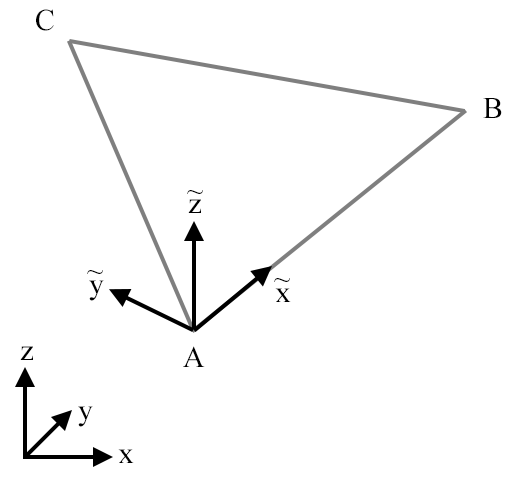
\includegraphics[width=0.4\linewidth]{figures/triangle}
  	\setlength\unitlength{0.80cm}
  	\begin{picture}(7.5,7.5)
  	\thicklines
  	\put(0,0){\vector(0,1){1}}
  	\put(1.1,0){$x$}
  	\put(0,0){\vector(1,0){1}}
  	\put(0,1.1){$z$}
  	\put(0,0){\vector(1,1){0.5}}
  	\put(0.6,0.6){$y$}      
  	\put(1.75,1.75){\vector(1,0.75){0.8}}
  	\put(2.65,1.95){$\tilde{x}$}
  	\put(1.75,1.75){\vector(-1,0.3){0.9}}
  	\put(0.55,1.75){$\tilde{y}$}
  	\put(1.75,1.75){\vector(0,1){1.0}}
  	\put(1.65,2.85){$\tilde{z}$}
  	\thinlines
  	\polyline(1.75,1.75)(7,5.8)(0.5,7)(1.75,1.75)
  	\put(1.5,1.3){$A$}
  	\put(7.20,5.7){$B$}
  	\put(0.0,6.9){$C$}
  	\end{picture}
  	\caption{Arbitrary triangle with nodes A, B and C, defined in global $xyz$ coordinate system. After transformation a new, local, $\tilde{x}\tilde{y}\tilde{z}$ coordinate system with node A in its origin, is created.}
  	\label{fig:triangle}
  \end{figure}
    
  Given a triangle with vertices $\vec{A} = (a_x, a_y, a_z)^T, \vec{B} = (b_x, b_y, b_z)^T$ and $\vec{C} = (c_x, c_y, c_z)^T$ ordered in counterclockwise direction, as shown in Figure \ref{fig:triangle}. Let $\vec{u}$ be the vector from node $\vec{A}$ to $\vec{B}$ and $\vec{v}$ be the vector from node $\vec{A}$ to $\vec{C}$:
  \begin{align*}
  \vec{u} &= \vec{B}-\vec{A} = \begin{pmatrix}
  b_x - a_x & b_y - a_y & b_z - a_z
  \end{pmatrix}^T\\
  \vec{v} &= \vec{C}-\vec{A} = \begin{pmatrix}
  c_x - a_x & c_y - a_y & c_z - a_z
  \end{pmatrix}^T
  \end{align*}
  First local unit vector:
  \begin{equation*}
   \vec{\tilde{x}} = \frac{1}{\left|\vec{u}\right|}\vec{u}
  \end{equation*}
  Second local unit vector:
  \begin{align*}
   \vec{\tilde{z}} &= \vec{u} \times \vec{v} \\
   \vec{\tilde{z}} &\leftarrow \frac{1}{\left|\vec{\tilde{z}}\right|}\vec{\tilde{z}}
  \end{align*}
  Third local unit vector:
  \begin{equation*}
   \vec{\tilde{y}} = \vec{\tilde{z}} \times \vec{\tilde{x}}
  \end{equation*}
  Define transformation matrix $\underline{T}$ as follows:
  \begin{equation}\label{eq:trafoT_tri}
   \underline{T} = \begin{pmatrix}
   \vec{\tilde{x}}^T\\ \vec{\tilde{y}}^T\\ \vec{\tilde{z}}^T
   \end{pmatrix} = \begin{pmatrix}
   \tilde{x}_x & \tilde{x}_y & \tilde{x}_z\\
   \tilde{y}_x & \tilde{y}_y & \tilde{y}_z\\
   \tilde{z}_x & \tilde{z}_y & \tilde{z}_z
   \end{pmatrix}
  \end{equation}
  Assembly of element's stiffness matrix needs partial derivatives. In order to get these derivatives with less computational effort, every triangle can be translated in such a way, that node $\vec{A}$ lies in the global origin before transforming it to local coordinates. Node $\vec{A}$ stays at $(0,\ 0,\ 0)$ coordinates which then simplifies getting the derivatives (see section \ref{sec:Impl-Details-Assembly}). It follows:
  \begin{align*}
   \vec{\tilde{A}} &= \begin{pmatrix}
   0 & 0 & 0
   \end{pmatrix}^T \\
   \vec{\tilde{B}} &= \begin{pmatrix}
   \tilde{b}_x & 0 & 0
   \end{pmatrix}^T \\
   \vec{\tilde{C}} &= \begin{pmatrix}
   \tilde{c}_x & \tilde{c}_y & 0
   \end{pmatrix}^T
  \end{align*}
  Node $\vec{A}$ will not be changed by the transformation with $\underline{T}$, $\vec{B}$ will be projected onto the local $x$-axis that is defined to be the normalized vector between $\vec{A}$ and $\vec{B}$. Node $\vec{C}$ will be projected onto the local $xy$-plane. One can see that the $z$-component vanishes by transforming into local space, thus generating the two dimensional local space.
  
  \begin{figure}[htbp] % Bild von bel. Viereck mit ABCD, IJKL, globalem KoSys, lokalem KoSys mit Ursprung auf Schnittpunkt der gestrichelten Linien von JL und IK\newline
  	\centering
  	%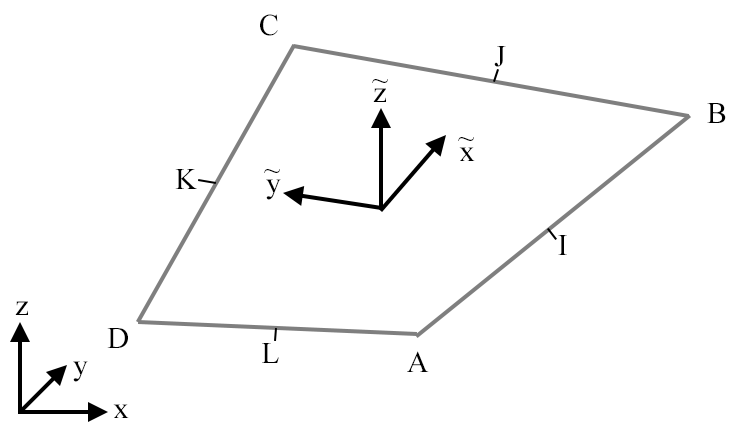
\includegraphics[width=0.5\linewidth]{figures/quadrilateral}
  	\setlength\unitlength{0.99cm}
  	\begin{picture}(7,5)
  	\thicklines
  	\put(0,0){\vector(0,1){1}}
  	\put(1.1,0){$x$}
  	\put(0,0){\vector(1,0){1}}
  	\put(0,1.1){$z$}
  	\put(0,0){\vector(1,1){0.5}}
  	\put(0.6,0.6){$y$}
  	\put(3.4,2.35){\vector(0.45,0.75){0.6}}
  	\put(4.1,3.0){$\tilde{x}$}
  	\put(3.4,2.35){\vector(-0.9,0.2){0.9}}
  	\put(2.25,2.65){$\tilde{y}$}
  	\put(3.4,2.35){\vector(0,1){1.0}}
  	\put(3.3,3.45){$\tilde{z}$}
  	\thinlines
  	\polyline(1,1)(4,0.5)(6.5,3.5)(2,4.5)(1,1)
  	\put(0.5,0.9){$D$}
  	\put(3.9,0){$A$}
  	\put(6.6,3.3){$B$}
  	\put(1.6,4.5){$C$}
  	\put(2.25,0.2){$L$}
  	\put(1.0,2.55){$K$}
  	\put(4.2,4.2){$J$}
  	\put(5.45,1.7){$I$}
  	\unitlength=0.99mm
  	\Dline(25,7.5)(43,40){1.5}
  	\Dline(52,19.5)(15,27.0){1.5}
  	\end{picture}
  	\caption{Quadrilateral with nodes A, B, C and D, defined in global $xyz$ coordinate system. After transformation a new, local, $\tilde{x}\tilde{y}\tilde{z}$ coordinate system is created.}
  	\label{fig:quadrilateral}
  \end{figure}
  
  The other element described in this work is the quadrilateral. Let an arbitrary quadrilateral be given with vertices $\vec{A} = (a_x,\ a_y,\ a_z)^T, \vec{B} = (b_x,\ b_y,\ b_z)^T, \vec{C} = (c_x,\ c_y,\ c_z)^T, \vec{D} = (d_x,\ d_y,\ d_z)^T$ ordered in counter-clockwise direction, cf. Figure \ref{fig:quadrilateral}. Next, let $\vec{I}$ be the midpoint of edge $\overline{AB}$:
  \begin{equation*}
   \vec{I} = \vec{A} + \frac{1}{2}\left( \vec{B}-\vec{A}\right)
  \end{equation*}
  Analogously let $\vec{J}, \vec{K}$ and $\vec{L}$ be the midpoints of the edges $\overline{BC}, \overline{CD}$ and $\overline{DA}$:
  \begin{align*}
   \vec{J} &= \vec{B} + \frac{1}{2}\left( \vec{C}-\vec{B}\right) \\
   \vec{K} &= \vec{C} + \frac{1}{2}\left( \vec{D}-\vec{C}\right) \\
   \vec{L} &= \vec{D} + \frac{1}{2}\left( \vec{A}-\vec{D}\right)
  \end{align*}
  Let then $\vec{u}$ be the vector from node $\vec{L}$ to $\vec{J}$ and $\vec{v}$ be the vector from node $\vec{I}$ to $\vec{K}$:
  \begin{align*}
   \vec{u} &= \vec{J}-\vec{L} = \begin{pmatrix}
   j_x-l_x & j_y-l_y & j_z-l_z
   \end{pmatrix}^T\\
   \vec{v} &= \vec{K}-\vec{I} = \begin{pmatrix}
   k_x-i_x & k_y-i_y & k_z-i_z
   \end{pmatrix}^T
  \end{align*}
  First local unit vector:
  \begin{equation*}
   \vec{\tilde{x}} = \frac{1}{\left|\vec{u}\right|}\vec{u}
  \end{equation*}
  Second local unit vector:
  \begin{align*}
   \vec{\tilde{z}} &= \vec{u} \times \vec{v}\\
   \vec{\tilde{z}} &\leftarrow \frac{1}{\left|\vec{\tilde{z}}\right|}\vec{\tilde{z}}
  \end{align*}
  Third local unit vector:
  \begin{equation*}
   \vec{\tilde{y}} = \vec{\tilde{z}} \times \vec{\tilde{x}}
  \end{equation*}
  Define transformation matrix $T$ as follows:
  \begin{equation}\label{eq:trafoT_quad}
   \underline{T} = \begin{pmatrix}
   \vec{\tilde{x}}^T\\ \vec{\tilde{y}}^T\\ \vec{\tilde{z}}^T
   \end{pmatrix} = \begin{pmatrix}
   \vec{\tilde{x}}_x & \vec{\tilde{x}}_y & \vec{\tilde{x}}_z\\ \vec{\tilde{y}}_x & \vec{\tilde{y}}_y & \vec{\tilde{y}}_z\\ \vec{\tilde{z}}_x & \vec{\tilde{z}}_y & \vec{\tilde{z}}_z
   \end{pmatrix}
  \end{equation}
  Remark: In order to transform a quadrilateral element from 3D to a local two dimensional space, the nodes of the original element must all be situated on a common plane. Otherwise such a transformation cannot be performed. Such shaped quadrilaterals cannot be used as shell elements.
 
 
 \subsection{Shell Element}\label{sec:Shell-Shell}
 % The combination of the two previous parts and the transformations results in the final shell element\newline
 Shell elements combine the capability of both, plane and plate elements. Every time a thin walled structure like a car body, dome structure or container with multi-axial pressures is to be simulated, shell elements provide a good solution. In this work only the so-called flat shell elements are described and used in the implementation. Details about curved shell elements, shells of revolution and general shells can be found in Cook et al. \cite{cook2002concepts}.
 
 Flat shell elements have a state of bending and membrane stress that can be described by superposition of the plane and plate element \cite{klein2013fem}. Figure \ref{fig:shell_triangle} shows the superposition of plane and plate elements to a flat shell element. The degrees of freedom of plane and plate at every node are combined at the node of the shell element. Obviously the plane and plate element must be of the same finite element's type, for example three node triangular or eight node quadrilateral.
 \begin{figure}[htbp] % bild wie bei 8.7 von scheibe und platte und kombination zu schale + erklärungen, welche unbekannten und kräfte man bei welchem teil hat
 	\centering
 	%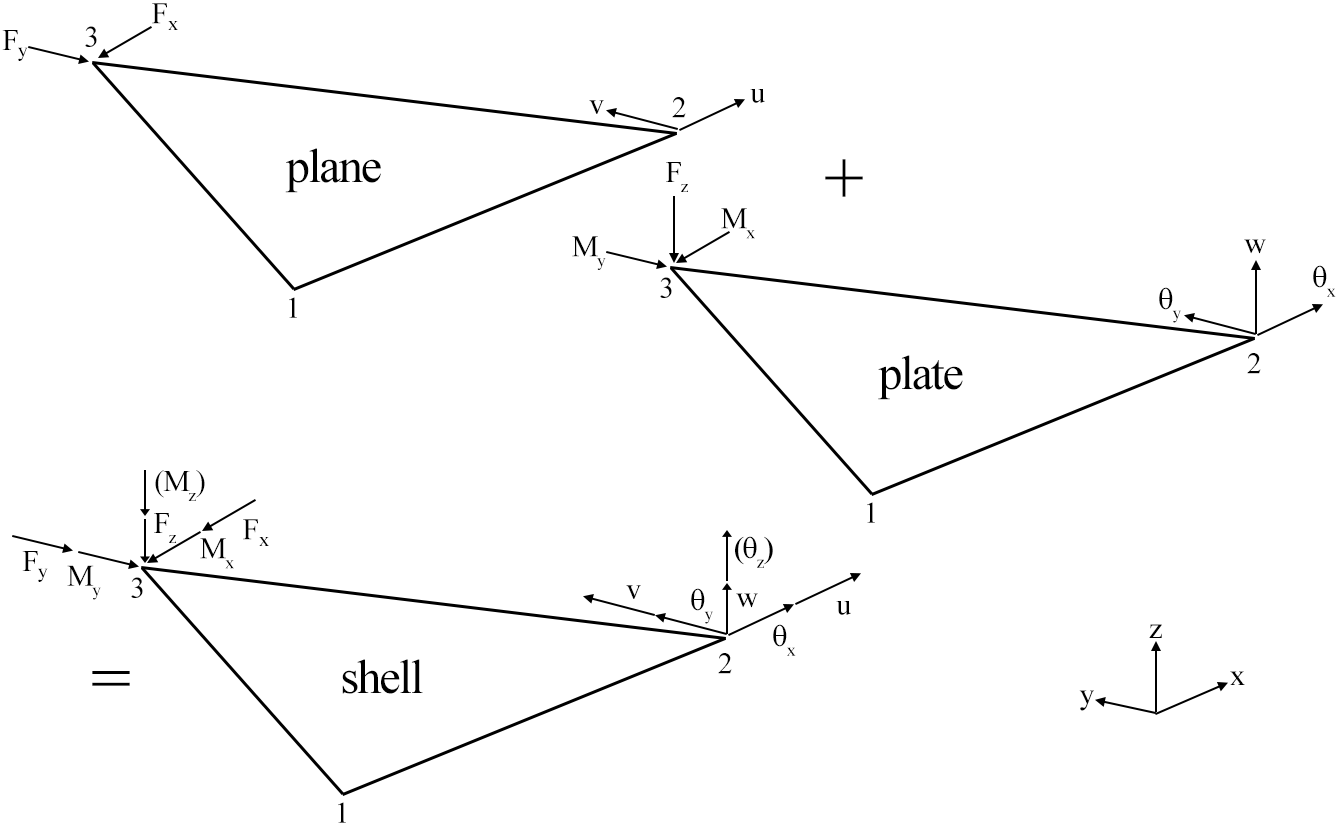
\includegraphics[width=0.8\linewidth]{figures/shell_triangle}
 	\setlength\unitlength{0.9cm}
 	\begin{picture}(11.5,9.5)
 	\thicklines
 	\put(10.0,3.5){\vector(1,0.5){0.55}}   \put(10.6,3.5){$x$}
 	\put(10.0,3.5){\vector(-0.5,1){0.25}}  \put(9.5,3.6){$y$}
 	\put(10.0,3.5){\vector(0,1){0.7}}      \put(9.9,4.3){$z$}
 	
 	\put(5.5,7.0){\vector(1,0.5){0.55}}   \put(6.0,6.9){$u$}
 	\put(5.5,7.0){\vector(-0.5,1){0.25}}  \put(4.8,7.3){$v$}
 	\put(1.55,8.8){\vector(-1,-0.5){0.55}}\put(1.4,8.45){$F_x$}
 	\put(0.7,9.0){\vector(0.5,-1){0.25}}  \put(0.3,8.45){$F_y$}
 	
 	\put(10.5,7.0){\vector(0,1){0.7}}     \put(10.6,7.3){$w$}
 	\put(10.5,7.0){\vector(1,0.5){0.55}}  \put(11.0,6.9){$\theta_x$}
 	\put(10.5,7.0){\vector(-0.5,1){0.25}} \put(9.8,7.3){$\theta_y$}
 	\put(6.0,9.2){\vector(0,-1){0.7}}     \put(6.1,8.9){$F_z$}
 	\put(6.55,8.8){\vector(-1,-0.5){0.55}}\put(6.4,8.45){$M_x$}
 	\put(5.7,9.0){\vector(0.5,-1){0.25}}  \put(5.3,8.45){$M_y$}
 	
 	\put(8.0,2.0){\vector(0,1){0.7}}      \put(8.1,2.3){$w$}
 	\put(8.0,2.0){\vector(1,0.5){0.55}}   \put(8.5,1.9){$\theta_x$}
 	\put(8.0,2.0){\vector(-0.5,1){0.25}}  \put(7.3,2.3){$\theta_y$}
 	\put(3.5,4.2){\vector(0,-1){0.7}}     \put(3.6,3.9){$F_z$}
 	\put(4.05,3.8){\vector(-1,-0.5){0.55}}\put(3.9,3.45){$M_x$}
 	\put(3.2,4.0){\vector(0.5,-1){0.25}}  \put(2.8,3.45){$M_y$}
 	\put(8.6,2.3){\vector(1,0.5){0.55}}   \put(9.0,2.2){$u$}
 	\put(7.75,2.5){\vector(-0.5,1){0.25}} \put(7.2,2.6){$v$}
 	\put(4.65,4.1){\vector(-1,-0.5){0.55}}\put(4.4,3.75){$F_x$}
 	\put(2.95,4.5){\vector(0.5,-1){0.25}} \put(2.6,3.9){$F_y$}
 	\put(8.0,2.7){\vector(0,1){0.7}}      \put(8.1,3.0){$(\theta_z)$}
 	\put(3.5,4.9){\vector(0,-1){0.7}}     \put(3.6,4.6){$(M_z)$}
 	\thinlines
 	\polyline(1.0,8.5)(2.5,5.5)(5.5,7.0)(1.0,8.5)
 	\put(2.3,5.1){$1$} \put(5.3,6.5){$2$} \put(0.8,8.0){$3$} 
 	\polyline(6.0,8.5)(7.5,5.5)(10.5,7.0)(6.0,8.5)
 	\put(7.3,5.1){$1$} \put(10.3,6.5){$2$} \put(5.8,8.0){$3$}  
 	\polyline(3.5,3.5)(5.0,0.5)(8.0,2.0)(3.5,3.5)
 	\put(4.8,0.1){$1$} \put(7.8,1.5){$2$} \put(3.3,3.0){$3$}
 	
 	\put(5.85,5.9){\textbf{{\Huge +}}} \put(2.3,1.5){\textbf{{\Huge =}}}
 	\end{picture}
 	\caption{Creation of a triangular flat shell element by superimposing a triangular plane and a triangular plate element. The elements are described in the same local coordinate system with their degrees of freedom shown exemplary at one node per element.}
 	\label{fig:shell_triangle}
 \end{figure} 
 The plane has displacements $u$ and $v$ with dedicated forces $F_x$ and $F_y$. The plate has the deformation $w$ with assigned normal force $F_z$ and the two twists $\theta_x$ and $\theta_y$ with assigned moments $M_x$ and $M_y$. Through the linking of the elements the shell element node has now five natural degrees of freedom. An additional twist around the local z-axis $\theta_z$ will be introduced \cite{steinke2005finite}, increasing the number to six degrees of freedom per node. In vector notation the resulting displacement vector $\vec{u}_i$ of a shell element's node $i$ is:
 \begin{align}\label{eq:shell_u_i}
 \vec{u} &= \underbrace{\begin{pmatrix}
 	u\\v\\w\\\theta_x\\\theta_y\\\theta_z
 	\end{pmatrix}} = \underbrace{\begin{pmatrix}
 	u\\v\\0\\0\\0\\0
 	\end{pmatrix}} + \underbrace{\begin{pmatrix}
 	0\\0\\w\\\theta_x\\\theta_y\\0
 	\end{pmatrix}} + \begin{pmatrix}
 0\\0\\0\\0\\0\\\theta_z
 \end{pmatrix}\\
 &\quad\;\; \text{shell}\ \quad\; \text{plane}\ \quad\! \text{plate}
 \end{align}
 
 % gesamtsteifigkeitsmatrix besteht aus blöcken (3x3 bei tri3, 4x4 bei quad4), Ku=F (gleichung 718 bei \cite{steinke2005finite})
 For the two different finite elements in this work - the three node triangular element and the four node quadrilateral element - the stiffness matrix for the shell element is described by a block matrix of either $3\!\times\!3$ submatrices for the triangular case or $4\!\times\!4$ submatrices for the quadrilateral. The following equation shows the latter case as example:
 \begin{align}\label{eq:shell_K_ij}
 \underline{K} \vec{u} &= \vec{F} \nonumber\\
 \begin{pmatrix}
 \underline{K}_{11} & \underline{K}_{12} & \underline{K}_{13} & \underline{K}_{14}\\
 \underline{K}_{21} & \underline{K}_{22} & \underline{K}_{23} & \underline{K}_{24}\\
 \underline{K}_{31} & \underline{K}_{32} & \underline{K}_{33} & \underline{K}_{34}\\
 \underline{K}_{41} & \underline{K}_{42} & \underline{K}_{43} & \underline{K}_{44}
 \end{pmatrix} \begin{pmatrix}
 \vec{u}_1 \\\vec{u}_2 \\\vec{u}_3\\\vec{u}_4
 \end{pmatrix} &= \begin{pmatrix}
 \vec{F}_1\\\vec{F}_2\\\vec{F}_3\\\vec{F}_4
 \end{pmatrix}
 \end{align}
 where the vectors $\vec{u}_i$ are the same as in equation \eqref{eq:shell_u_i}. The single submatrices $\underline{K}_{ij}$ of $\underline{K}$ were created by the superposition of the stiffness matrices of the plane and the plate:
 \begin{equation}
 \underline{K}_{ij} = \left(\underline{\hat{K}}_{ij}\right)_m + \left(\underline{\hat{K}}_{ij}\right)_p
 \end{equation}
 The submatrix $\underline{K}_{ij}$ has the following structure:
 \begin{align}
 \begin{gmatrix}[p]
 \circ & \circ & 0     & 0     & 0     & 0 \\
 \circ & \circ & 0     & 0     & 0     & 0 \\
 0     & 0     & \star & \star & \star & 0 \\
 0     & 0     & \star & \star & \star & 0 \\
 0     & 0     & \star & \star & \star & 0 \\
 0     & 0     & 0     & 0     & 0     & 0
 \colops
 \mult{0}{u}
 \mult{1}{v}
 \mult{2}{w}
 \mult{3}{\theta_x}
 \mult{4}{\theta_y}
 \mult{5}{\theta_z}
 \rowops
 \mult{0}{u}
 \mult{1}{v}
 \mult{2}{w}
 \mult{3}{\theta_x}
 \mult{4}{\theta_y}
 \mult{5}{\theta_z}
 \end{gmatrix} &= \begin{gmatrix}[p]
 \circ & \circ & 0 & 0 & 0 & 0 \\
 \circ & \circ & 0 & 0 & 0 & 0 \\
 0     & 0     & 0 & 0 & 0 & 0 \\
 0     & 0     & 0 & 0 & 0 & 0 \\
 0     & 0     & 0 & 0 & 0 & 0 \\
 0     & 0     & 0 & 0 & 0 & 0
 \colops
 \mult{0}{u}
 \mult{1}{v}
 \mult{2}{w}
 \mult{3}{\theta_x}
 \mult{4}{\theta_y}
 \mult{5}{\theta_z}
 \rowops
 \mult{0}{u}
 \mult{1}{v}
 \mult{2}{w}
 \mult{3}{\theta_x}
 \mult{4}{\theta_y}
 \mult{5}{\theta_z}
 \end{gmatrix} + \begin{gmatrix}[p]
 0     & 0     & 0     & 0     & 0     & 0 \\
 0     & 0     & 0     & 0     & 0     & 0 \\
 0     & 0     & \star & \star & \star & 0 \\
 0     & 0     & \star & \star & \star & 0 \\
 0     & 0     & \star & \star & \star & 0 \\
 0     & 0     & 0     & 0     & 0     & 0
 \colops
 \mult{0}{u}
 \mult{1}{v}
 \mult{2}{w}
 \mult{3}{\theta_x}
 \mult{4}{\theta_y}
 \mult{5}{\theta_z}
 \rowops
 \mult{0}{u}
 \mult{1}{v}
 \mult{2}{w}
 \mult{3}{\theta_x}
 \mult{4}{\theta_y}
 \mult{5}{\theta_z}
 \end{gmatrix}
 \end{align}
 % Sei $K_m$ die lokale Steifigkeitsmatrix vom Membran/Plane-Teil und $K_p$ die vom Plate-bending-Teil
 
 % Kij weisst in der Spalte theta\_z und Zeile theta\_z $(k_ij)_66$ eine null auf -> erklärung und warum schlecht. ANDERE REFERENZ ERKLÄRT, WAS WIR DESHALB MACHEN (1/1000 der diagonalwerte)
 $\left(\underline{\hat{K}}_{ij}\right)_m$ describes the submatrix of the stiffness matrix of the plane element for node $i$ and $j$ and is marked with the $\circ$-symbol, $\left(\underline{\hat{K}}_{ij}\right)_p$ describes the corresponding matrix part of the plate element's stiffness matrix and is symbolized with a $\star$.
 The degree of freedom $\theta_z$ does not exists in both, the plane and the plate element, and were introduced with the shell element. Therefore $(\underline{K}_{ij})_{66}$ is zero. The sixth degree of freedom is necessary because the missing stiffness regarding a rotation around the axis normal to the element could produce singularities in the overall stiffness matrix. This happens for example, if all neighboring elements of a node lie in the same plane, i.e. they are coplanar. A singularity can lead to a non-solvable system, so this case needs be excluded \cite{steinke2005finite}. One way is to introduce this sixth degree of freedom and give it a value that is so small that it does not influence the displacements and stresses too much. The number of this values varies: Werkle suggests a value of $1/10000$ of the smallest diagonal entry of $\underline{K}_{ij}$ \cite{werkle1995finite}, whereas \cite{kansara2004development} used $1/1000$ of the smallest diagonal entry of $\underline{K}_{ij}$. The value must be small, but big enough to prevent the singularities. Since this value is an approximation, one has to modify it, if the solution is not as expected or one cannot get a solution at all due to the addressed singularities.
 
 % Dann muss die (Rück-)Transformationsmatrix $T$ erstellt werden, da SKM im lokalen KoSys definiert ist, aber in die globale Systemmatrix einsortiert werden muss
 The stiffness matrix for the shell element was constructed in a local coordinate system as described in section \ref{sec:Shell-Plane}, \ref{sec:Shell-Plate} and \ref{sec:Shell-CoTrafo}. The overall stiffness matrix containing information about all elements need to be described in a global coordinate system. Before the element stiffness matrix is added to the global stiffness matrix, it has to be transformed from local to global. This can be achieved by transforming the single blocks of $\underline{K}$ from equation \eqref{eq:shell_K_ij} with the relation:
 \begin{equation}\label{eq:shell_K_ij u_j=F_i}
 \underline{\check{K}}_{ij} \vec{\check{u}}_j = \vec{\check{F}}_i
 \end{equation}
 where ``\;$\check{\ }$\;'' denotes that the matrix and vector are represented in local coordinates. With the help of the transformation matrix $\underline{\tilde{T}}$, the globally described displacement vector $\vec{u}_j$ and load vector $\vec{F}_i$ can be represented in local coordinates:
 \begin{align}
 \check{\vec{u}}_j = \underline{\tilde{T}} \vec{u}_j\\
 \check{\vec{F}}_i = \underline{\tilde{T}} \vec{F}_i
 \end{align}
 Since the load vector is to be defined in a global coordinate system and the resulting displacements are to be defined globally, too, equation \eqref{eq:shell_K_ij u_j=F_i} will be multiplied by $\underline{\tilde{T}}^T$ from left:
 \begin{equation}
 \underline{\tilde{T}}^T \underline{\check{K}}_{ij} \underline{\tilde{T}} \vec{u}_j = \underline{\tilde{T}}^T \underline{\tilde{T}} \vec{F}_i = \vec{F}_i
 \end{equation}
 Hence, the two vectors will be represented in global coordinates and only the local element stiffness matrix need to be transformed. The addressed $6\!\times\!6$ transformation matrix $\underline{\tilde{T}}$ is made up of the $3\!\times\!3$ transformation matrix $\underline{T}$ from section \ref{sec:Shell-CoTrafo}:
 \begin{equation}\label{eq:trafoTtilde}
 \underline{\tilde{T}} = \begin{pmatrix}
 \underline{T} & 0\\
 0 & \underline{T}
 \end{pmatrix}
 \end{equation}
 
 % Je nachdem ob 3 oder 4 Knotenelement (Tri-3/Quad-4) sieht $K$ und $T$ natürlich anders aus
 In order to get the local element stiffness matrix $\underline{K}$ transformed to the global coordinate system, one has to transform the single submatrices $\underline{K}_{ij}$ as follows:
 \begin{equation}\label{eq:Kij=Tt Kij T}
 \underline{K}_{ij} = \underline{\tilde{T}}^T \underline{\check{K}}_{ij} \underline{\tilde{T}}
 \end{equation}
 for $1 \leq i,j \leq 3$ in the case of the triangular element and $1 \leq i,j, \leq 4$ for the quadrilateral element, respectively.
 \newpage
\cleardoublepage

\section{FEM Code Implementation}
 This section contains information about the features of the framework ``libMesh'' that was used in the implementation of the program, details on important parts of the implementation like the system matrix assembly or the mesh format requirements and import. Additionally the parallelization with MPI concludes this section, describing details about libMesh requirements for MPI usage and important modifications to the program's code.
 
 
 
 \subsection{Introduction to libMesh}\label{sec:Impl-Intro}
 The libMesh finite element library was stared as part of the Ph.D. work of Benjamin Kirk \cite{kirk2007adaptive}. It is a tool for numerical simulation of partial differential equations on serial and parallel platforms and uses the finite element method. Major goals are to provide data structures and algorithms for applications that need implicit numerical methods, parallel computing, adaptive mesh refinement techniques, or, a combination of them. Further, it simplifies many programming details for the user, such as: Reading the mesh from file, initialize data structures, solving the dicretized system, and, writing out the results \cite{kirk2013case}.
 
 LibMesh allows discretization of one, two and three dimensional problems using several geometric element types, including: Edges, quadrilaterals, triangles, tetrahedra, hexahedra, pyramids, prisms and some infinite elements of quadrilaterals or hexahedra. Finite elements include traditional first and second order Lagrange, as well as arbitrary order hierarchical bases, and N\'{e}d\'{e}lec elements of first type.
 
 Mesh partitioning is available in libMesh through interfaces to several external packages, but also some internal partitioning algorithms are provided: Linear and centroid partitioner as examples of internal algorithms, Metis and ParMetis \cite{karypis1998fast} as examples for external partitioner. In addition to these two, libMesh includes interfaces to solver libraries such as PETSc \cite{petsc2015url} and LASPack \cite{laspack2015url}. Thus, libMesh provides several linear equation solvers such as GMRES, CG, Bi-CGSTAB, QMR, and preconditioners like Jacobi, incomplete LU factorization and incomplete Cholesky factorization. The choice of an appropriate solver and preconditioner is made by the user at runtime.
 
 A wide variety of mesh formats are supported by libMesh to facilitate use of complex geometries. The following is an incomplete list of supported input and output formats: Nemesis, TetGen, I-deas Universal UNV, AVS's ASCII UCD, Visualization Toolkit VTK, libMesh formats XDR/XDA, ExodusII, GMSH, LANL's General Mesh Viewer GMV, GnuPlot (only output), Matlab (only input) \cite{kirk2013case}.
 
 An example program using the libMesh library would look like listing \ref{lst:example-libmesh}.
 \begin{lstlisting}[caption=Example libMesh program,label=lst:example-libmesh]
#include "libmesh/libmesh.h"
#include "libmesh/additional_libmesh_components"

using namespace libMesh;

void assemble_something(EquationSystems& es, const std::string& system_name);

int main (int argc, char** argv)
{
	LibMeshInit (int argc, char** argv);
	
	Mesh mesh( init.comm() );
	
	// mesh generation via MeshTools::Generation::build_... or mesh import from file via mesh.read(std::string filename)
	
	EquationSystems es(mesh);
	
	LinearImplicitSystem& system = es.add_system<LinearImplicitSystem> ("example system");
	
	system.add_variable ("a", FIRST);
	system.add_variable ("b", SECOND, LAGRANGE);
	
	system.attach_assemble_function (assemble_something);

	es.init();
	
	system.solve();
	
	VTKIO (mesh).write_equation_systems ("out.pvtu", es);
	
	return 0;
}
 \end{lstlisting}
 In fact, this is the base construction of nearly every libMesh program. It starts with including libMesh components that are needed by the program, e.g. \textit{mesh.h, equation\_systems.h, fe.h}. Then, the library needs to be initialized (line 10). This is necessary because it may depend on a number of other external libraries like MPI and PETSc that require initialization before use. On the other hand, if the \texttt{\textbf{LibMeshInit}} object goes out of scope, the other libraries are finalized automatically by libMesh. Next, a mesh is created (lines 12-14) on the default MPI communicator (even if the program is executed single-threaded). The mesh can either be read from file or created by internal mesh generation tools. In line 16 an equation systems object is created. It can contain multiple different systems. Here, only one linear implicit system is added to the object (line 16). Each system can contain multiple variables of different approximation orders (see lines 20/21). Many systems require a user-defined function that will assemble the (linear) system (lines 6 and 23). Now, the data structures for equation system must be initialized which is done in line 25. The solving of the systems is done in line 27 of the code. This one line of code calls the assemble function defined earlier and invokes the default numerical solver. If the external library PETSc is installed, the solver can be controlled from the command line by the user. After solving the system, the solution can be written to file; here, for example, the results are written to a VTK-formatted plot file (line 29).
 
 \subsection{Implementation Details}\label{sec:Impl-Details}
  This section contains details about the program's implementation using the libMesh framework. Different parts of the code like the initialization, loading of the mesh or assembling of the system matrix are described. The focus is put on the interaction between the libMesh library and the user's code. Requirements regarding mesh formats and user arguments are described as well.

 
  \subsubsection{Initialization}\label{sec:Impl-Details-Init}
  The program expects a few parameters set by the user through the command line at start. The ordering of these parameters are not relevant; some are optional. Here is a complete list of all parameters that can be set in the command line:
  \begin{itemize}
  	\item \textbf{-nu}: The Poisson's ratio $\nu$ is required by the material matrices. A value in the range $0.0 < \nu \leq 0.5$ is recommended for most scenarios.
  	\item \textbf{-e}: The elastic modulus or Young's modulus $E$ is also required by the material matrices. Here, a value $E \gg 0$ is recommended.
  	\item \textbf{-t}: The thickness $t$ of the mesh. It is used at both, the material matrices and the strain-displacement matrices and thus a required parameter to be set by the user.
  	\item \textbf{-d}: If set to "`1"' additional messages regarding transformation matrix entries, strain-displacement matrices, force load vectors and other internal mathematic structures are put out on the console. This parameter is optional, as it only gives the user more information in case of finding error. Since it slows down the calculation, it should only be set if needed. To turn off the messages, simply ignore the parameter or set it to 0.
  	\item \textbf{-mesh}: The file name of the mesh file to be imported. A required parameter, because no default mesh is coded into the program to be used. The relative path to the file (+ extension) must be specified. Allowed file formats are: libMesh format \textit{xda} (ASCII) and \textit{xdr} (binary) as well as GMSH format \textit{msh}. For more details, see section \ref{sec:Impl-Details-MeshFileImport}.
  	\item \textbf{-out}: The relative path and filename (\textit{without} extension) for the output of the resulting mesh. This parameter is optional. If not set, no output file will be created. The path to the filename must exist, otherwise no file can be created.
  \end{itemize}
  
  If the external library PETSc is installed and libMesh is configured to be able to use it, the user can set additional optional parameters \cite{petsc-user-ref}. In fact, if one uses PETSc, it will look though all command line arguments by itself to find those it can process. The following list is therefore limited to parameters that directly coincide with the need of this program. For more PETSc command line argument see \cite{petsc-user-ref}.
  \begin{itemize}
  	\item \textbf{-ksp\_type}: Specifies the Krylov subspace method. Options are: \texttt{richardson}, \texttt{chebyshev}, \texttt{cg}, \texttt{gmres}, \texttt{tcqmr}, \texttt{bcgs}, \texttt{cgs}, \texttt{tfqmr}, \texttt{cr}, \texttt{lsqr}, \texttt{bicg}, \texttt{preonly}.
  	\item \textbf{-pc\_type}: To employ a particular preconditioning method used with the Krylov space method, the user can select one using this command line argument. Options are: \texttt{none}, \texttt{jacobi}, \texttt{bjacobi}, \texttt{sor}, \texttt{eisenstat}, \texttt{icc}, \texttt{ilu}, \texttt{asm}, \texttt{gasm}, \texttt{gamg}, \texttt{bddc}, \texttt{ksp}, \texttt{composite}, \texttt{lu}, \texttt{cholesky}, \texttt{shell}. 
  \end{itemize}
   
   
   
  \subsubsection{Mesh file import}\label{sec:Impl-Details-MeshFileImport}
   The mesh geometry needs to be defined in a mesh file. LibMesh can import meshes from many different formats, including its own libMesh formats XDA and XDA, the first one stored in readable ASCII format, the latter one stored as binary code. Another one is the GMSH format \textit{msh}. There are other formats libMesh can import, but only the three mentioned formats are currently supported by the thesis' program.
   A mesh file must provide the following information in order to be usable be the implementation:
   \begin{itemize}
   	\item A list of vertices. Every vertex must be specified with its $xyz$-coordinates defined in the global coordinate system.
   	\item A list of elements the mesh consists out of. The elements are normally defined by their type, for example three node triangle or four node quadrilateral, and a list of vertex identifiers representing the nodes of the element.
   	\item A list of boundary conditions. The program provides two different types of boundary conditions. The type is to be specified in form of identifiers on element's nodes or edges. In the latter case the boundary condition is used on both nodes defining the edge.
   \end{itemize}
   Listing \ref{lst:xda} shows a short example of a mesh defined in the xda-format. It represents the unit square with its center at the global origin, composed of two three node triangles. It has different boundary conditions on the bottom and top edge.
\begin{lstlisting}[caption=Example xda mesh file,label=lst:xda,language=bash,keepspaces=true]
libMesh-0.7.0+
2       # number of elements
4       # number of nodes
.       # boundary condition specification file
n/a     # subdomain id specification file
n/a     # processor id specification file
n/a     # p-level specification file
2       # n_elem at level 0, [ type (n0 ... nN-1) ]
3 0 1 2          # 3 -> triangle with 3 nodes, 0 1 2 -> vertices 0, 1 and 2
3 1 3 2          #                             1 3 2 -> vertices 1, 3 and 2
-1.0 -1.0  0.0   # x y z coordinates of vertex 0
 1.0 -1.0  0.0   #                      vertex 1
-1.0  1.0  0.0   #                      vertex 2
 1.0  1.0  0.0   #                      vertex 3
2                # number of boundary conditions
0 0 1            # 0 -> element 0, 0 -> edge 0 (between vertex 0 and 1), bc-type 1
1 1 0            # 1 -> element 1, 1 -> edge 1 (between vertex 3 and 2), bc-type 0
\end{lstlisting}
   Listing \ref{lst:msh} shows the same example but in the GMSH format. Here, libMesh has some requirements how the GMSH mesh file has to be structured: Every line defined in the \texttt{\$Elements}-section contains severals numbers, ordered as follows: Element index, element type, number of tags, physical entity number, geometrical entity, additional list of tags, list of node indices \cite{gmsh-manual}. LibMesh requires the number of tags to be at least two. The first tag (physical entity) will be used by libMesh to identify the boundary condition ID; the second tag will be ignored - at least the author could not find where libMesh uses this value. LibMesh also treats the element type in different ways: The highest dimensional element types, for example 2D elements, like triangle and quadrilaterals, will act as the mesh defining elements. Every element that has lower dimension, i.e. nodes or edges, for instance, will be seen as boundary condition definitions by libMesh. See listing \ref{lst:msh}: There are six elements defined: Two triangles and four single nodes. The mesh only exists out of the two triangles. The four nodes will be used by libMesh to set boundary conditions at the corresponding nodes of the mesh. In this case node 1 and 2 gets boundary conditions with ID 0, node 3 and 4 with ID 1. This behavior of libMesh must be kept in mind when dealing with GMSH mesh files.
\begin{lstlisting}[caption=Example GMSH mesh file,label=lst:msh,language=bash,keepspaces=true]
$MeshFormat
2.2 0 8
$EndMeshFormat
$Nodes
4
1 -1.0 -1.0  0.0
2  1.0 -1.0  0.0
3 -1.0  1.0  0.0
4  1.0  1.0  0.0
$EndNodes
$Elements
6
1 2 2 0 0 1 2 3
2 2 2 0 0 2 4 3
3 15 2 0 0 1
4 15 2 0 0 2
5 15 2 1 0 3
5 15 2 1 0 4
$EndElements
\end{lstlisting}

   The program features two different types of boundary conditions whose identifier must be set in the mesh file:
   \begin{itemize}
   	\item Simply supported boundaries has type ``\texttt{0}''. This means that the boundary cannot be moved but is free to rotate and have no moment resistance. In mathematical notation: $u = v = w = 0, M_x = M_y = 0$.
   	\item Clamped boundary has type ``\texttt{1}''. Here, the boundary is completely fixed with no movement and no rotation possible. Mathematically: $u = v = w = 0, \theta_x = \theta_y = 0$
   \end{itemize}
   
   Because the stand-alone version of the program has no coupled fluid solver which provides it with pressures/forces and moments at the nodes, these values must be imported via file, too. The structure of such a file is fairly simple: Listing \ref{lst:example_f} shows such an example corresponding to the example mesh of listing \ref{lst:xda}. The first line defines the number $n$ of nodes/vertices the mesh has (in this case $n=4$). The second line holds a floating point number representing a global factor that is multiplied by every force/moment component defined below. A value of $1.0$ has no effect on the load values. Lines three to $n+2$ are the $xyz$-components of the single forces put on the corresponding mesh nodes followed by three values for the moments $M_x, M_y, M_z$. The ordering is the same as the vertices in the mesh file. The $xyz$-coordinates must also be represented in the global coordinate system. In the example a load is applied on the first and third node. The first load is directed along the negative z-axis, the second load along the positive y-axis. The other two nodes have no forces or moments applied.
\begin{lstlisting}[caption=Example force file,label=lst:example_f,language=bash,keepspaces=true]
4
1.0
0.0  0.0  -0.65  0.0  0.0  0.0
0.0  0.0   0.0   0.0  0.0  0.0
0.0  2.34  0.0   0.0  0.0  0.0
0.0  0.0   0.0   0.0  0.0  0.0
\end{lstlisting}
   
   The implementation's code to import a mesh file is rather short (listing \ref{lst:load_mesh}).
\begin{lstlisting}[caption=Loading mesh and prepare for use,label=lst:load_mesh,keepspaces=true]
Mesh mesh(init.comm(), 2);
mesh.allow_renumbering(false);
mesh.read(in_filename);	
mesh.print_info();
\end{lstlisting}   
   The first line creates a 2D mesh distributed across the default MPI communicator (gathered by the \texttt{LibMeshInit}-object). The mesh is read in line 3 from the file found at the place defined by \texttt{in\_filename}. In line 4 information about the mesh is printed to the console. A special detail is line 2: It is not guaranteed that the ordering of the nodes defined in the mesh file is the same after libMesh has imported the mesh file. Since the program uses the additional force file to apply the loads onto the mesh nodes, this mapping could be destroyed. Therefore the function call in line 2 forbids libMesh to automatically renumber the nodes of the mesh and let the ordering be as defined in the mesh file.


  \subsubsection{System setup}\label{sec:Impl-Details-SystemSetup}
  After libMesh and possible external libraries are initialized and the mesh was created and initialized, the equation system must be set up. Listing \ref{lst:setup_system} shows the relevant part of the implementation.
\begin{lstlisting}[caption=Setting up the equation system,label=lst:setup_system,keepspaces=true]
EquationSystems equation_systems (mesh);
LinearImplicitSystem& system = equation_systems.add_system<LinearImplicitSystem> ("Elasticity");

unsigned int u_var  = system.add_variable("u",  FIRST, LAGRANGE);
unsigned int v_var  = system.add_variable("v",  FIRST, LAGRANGE);
unsigned int w_var  = system.add_variable("w",  FIRST, LAGRANGE);
unsigned int tx_var = system.add_variable("tx", FIRST, LAGRANGE);
unsigned int ty_var = system.add_variable("ty", FIRST, LAGRANGE);
unsigned int tz_var = system.add_variable("tz", FIRST, LAGRANGE);

system.attach_assemble_function (assemble_elasticity);

std::set<boundary_id_type> boundary_ids;
boundary_ids.insert(0);
std::vector<unsigned int> variables;
variables.push_back(u_var);
variables.push_back(v_var);
variables.push_back(w_var);
ConstFunction<Number> cf(0.0);
DirichletBoundary dirichlet_bc(boundary_ids, variables, &cf);

boundary_ids.clear();
boundary_ids.insert(1);
variables.push_back(tx_var);
variables.push_back(ty_var);
variables.push_back(tz_var);
DirichletBoundary dirichlet_bc2(boundary_ids, variables, &cf);

system.get_dof_map().add_dirichlet_boundary(dirichlet_bc);
system.get_dof_map().add_dirichlet_boundary(dirichlet_bc2);

equation_systems.init();
equation_systems.print_info();
\end{lstlisting}
   In line 1 an \texttt{EquationSystems}-object is created. It contains and controls all equation systems defined for a mesh, that is passed as parameter in its constructor. It can have multiple systems or just one like in this case. In this implementation a linear implicit system is used. LibMesh provides a system with the exact same name. In line 2 such a system is created named ``Elasticity'' and added to the equation systems. As discussed in section \ref{sec:Shell-Shell} the systems has six variables, namely: $u, v, w, \theta_x, \theta_y, \theta_z$. These variables are added to the system in the lines 4 to 9. All of them are of first polynomial order and members of the Lagrange finite element family. The \texttt{add\_variable}-functions returns a unique number identifying the variable just added. In order to assemble the system matrix and the right-hand side, a user-defined function must be attached to the system. This is done in line 11. The assemble function is part of section \ref{sec:Impl-Details-Assembly}. The only thing missing is the definition of the different boundary conditions. This is done between the lines 13 and 30. As stated in the previous section, the program features two type of boundary conditions: Simply supported and clamped with the ID ``0'' and ``1'', respectively. Because libMesh allows multiple IDs represent the same boundary condition type, in line 13 a set is created and filled with the 0-ID in the next line. After that, a vector containing the IDs of the system's variables must be created. For the simply supported boundary case, only the three displacement variables $u,v,w$ are affected (lines 15-18). Before creating the \texttt{DirichletBoundary}-object, a function supplying the Dirichlet value must be defined. In this case the value must be zero at the boundary. A \texttt{ConstFunction} initialized with the value zero is therefore created in line 19. The constructor for the Dirichlet object takes the ID-set, the variables-vector and the function as parameters and copies their content into its object. The set and vector will be reused for the second boundary type. Now the 1-ID is inserted in the cleared set in line 23 and the twist variables $\theta_x, \theta_y, \theta_z$ are added to the existing variables in the vector (lines 24ff). Another \texttt{DirichletBoundary} object is created with the new initialization parameters. Finally, the two boundary types are added to the system in the lines 29 and 30. When the preparation steps are finished, the system can finally be initialized and information about the system can be print to the console.
     

   
  \subsubsection{Matrix and vector assembly}\label{sec:Impl-Details-Assembly}
  As stated in section \ref{sec:Impl-Intro}, libMesh tries to do as much programming tasks as possible on its own and let the user concentrate on the mathematical/physical problem to model. The last sections show that this is often true, since the user often only need to set parameters, create objects or call functions. To solve the system, libMesh calls a user-defined assembly function. This function is the part where the user is involved at most, because here the system matrix and the right-hand side (RHS) must be assembled. Nevertheless libMesh helps the user with many auxiliary function as can be seen further down. The main part of the assembly function is described in listing \ref{lst:assemble}.
\begin{lstlisting}[caption=Assemble System Matrix and RHS,label=lst:assemble,float]
LinearImplicitSystem& system = es.get_system<LinearImplicitSystem>("Elasticity");
const DofMap& dof_map = system.get_dof_map();

DenseMatrix<Number> Ke, Ke_m, Ke_p;
DenseVector<Number> Fe;
DenseMatrix<Real> trafo;
DenseMatrix<Real> transUV;
DenseMatrix<Real> dphi;
Real area = 0.0;

std::vector<dof_id_type> dof_indices;
std::unordered_set<dof_id_type> processedNodes;
processedNodes.reserve(mesh.n_local_nodes());

MeshBase::const_element_iterator       el     = mesh.active_local_elements_begin();
const MeshBase::const_element_iterator end_el = mesh.active_local_elements_end();
for (; el != end_el; ++el)
{
	const Elem* elem = *el;
	dof_map.dof_indices (elem, dof_indices);
	ElemType type = elem->type();

	initElement(&elem, transUV, trafo, dphi, &area);

	calcPlane(type, transUV, dphi, &area, Ke_m);
	calcPlate(type, dphi, &area, Ke_p);
	constructStiffnessMatrix(type, Ke_m, Ke_p, Ke);
	localToGlobalTrafo(type, trafo, Ke);
	contribRHS(&elem, Fe, &processedNodes);

	dof_map.constrain_element_matrix_and_vector(Ke, Fe, dof_indices);

	system.matrix->add_matrix (Ke, dof_indices);
	system.rhs->add_vector    (Fe, dof_indices);
}
\end{lstlisting}
   The first step is to get a reference to the system whose matrix and vector needs to be assembled. In this case the ``Elasticity'' system is used (line 1). Next a reference to a special object is get from the system: The \texttt{DofMap}-object handles the numbering of degrees of freedom on a mesh. In line 3 to 9 several variables are defined: \texttt{Ke}, \texttt{Ke\_m} and \texttt{Ke\_p} are matrices representing the shell element's stiffness matrix, plane (or \textbf{m}embrane) stiffness matrix part and \textbf{p}late stiffness matrix part, respectively. The values of the element's RHS are stored in the vector \texttt{Fe}. The over three matrices are needed for the transformation of the element to local coordinates (\texttt{trafo}), the storing of the transformed nodes (\texttt{transUV}) and the partial derivatives (\texttt{dphi}). The element's area is stored in the variable of the same name.

   The assembly function creates the local stiffness matrix and RHS for every single finite element and adds it to the global system matrix and system right-hand side. Therefore one has to iterate over all elements. This is done in line 15 to 35. The following steps are made in the exact same order:
   \begin{itemize}
   	\item Get the mapping of the element's degrees of freedom to their positions in the system matrix (line 20)
   	\item Transform the element from global to local coordinates, calculate its partial derivatives and its area (line 23)
   	\item Assemble the plane stiffness matrix part of the shell element (line 25)
   	\item Assemble the plate stiffness matrix part of the shell element (line 26)
   	\item Construct the shell stiffness matrix for the current element (line 27)
   	\item Transform the local shell stiffness matrix back to global coordinates (line 28)
   	\item Apply possible forces to the element in the form of contribution to the local RHS (line 29)
   	\item Constrain the local element's stiffness matrix and RHS according to the set boundary conditions (line 31): LibMesh provides a function that automatically constrains the system matrix and right-hand side vector due to the boundary condition definitions in the initialization step.
    \item Add the element's stiffness matrix to the global system matrix (line 33): The final element's stiffness matrix is added to the overall system matrix through the function provided by libMesh. The vector storing the mappings of the degrees of freedom ensures that the matrix is added at the correct position in the system matrix.
    \item Add the element's RHS to the global RHS (line 34): Same as before but now for the right-hand side vector.
   \end{itemize}
   The transformation from global to local coordinates is described in section \ref{sec:Shell-CoTrafo}. Let $\tilde{A} = \begin{pmatrix}
   x_1=0 & y_1=0
   \end{pmatrix}^T, \tilde{B} = \begin{pmatrix}
   x_2 & y_2=0
   \end{pmatrix}^T, \tilde{C} = \begin{pmatrix}
   x_3 & y_3
   \end{pmatrix}$ be the nodes of a transformed triangular element. Then the partial derivatives are as follows:
   \begin{align*}
   x_{12} = x_1 - x_2 = -x_2 &\qquad y_{12} = y_1 - y_2 = 0\\
   x_{31} = x_3 - x_1 = x_3  &\qquad y_{31} = y_3 - y_1 = y_3\\
   x_{23} = x_2 - x_3        &\qquad y_{23} = y_2 - y_3 = -y_3
   \end{align*}
   For a transformed quadrilateral the derivatives are straightforward: $x_{ij} = x_i - x_j, y_{ij} = y_i - y_j$, because no implicit positions can be assumed for the transformed nodes.
   
   The area of a triangle can easily be calculated during the creation of the transformation matrix. The cross product between the spanning vectors $\vec{u}$ and $\vec{v}$ (cf. section \ref{sec:Shell-CoTrafo}) is 2 times the area of the triangle. Thus, the area is:
   \begin{equation*}
   A_\triangle = \frac{1}{2} \left|\vec{u} \times \vec{v}\right|
   \end{equation*}
   For the quadrilateral area $A_\square$ one can use the Gauss' area formula:
   \begin{equation*}
   A_\square = \frac{1}{2} \sum_{i=1}^{4} \left|\begin{pmatrix}
   x_i & x_{(i+1)\%4}\\
   y_i & y_{(i+1)\%4}
   \end{pmatrix}\right|
   \end{equation*}
   where ``\%'' represents the modulo-operator.
   
   After the assembly of the plane stiffness part described in section \ref{sec:Shell-Plane-Tri} for triangular elements and in \ref{sec:Shell-Plane-Quad} for quadrilateral elements, a matrix $K_m$ with $2n\!\times\! 2n$ entries results, $n$ being the number of nodes the element has:
   \begin{equation*}
   K_m = \begin{gmatrix}[p]
   m_{1,1} & m_{1,2} & m_{1,3} & \cdots & m_{1,n-1} & m_{1,n} \\
   m_{2,1} & m_{2,2} & m_{2,3} & \cdots & m_{2,n-1} & m_{2,n} \\
   m_{3,1} & m_{3,2} & m_{3,3} & \cdots & m_{3,n-1} & m_{3,n} \\
   \vdots & \vdots & \vdots & \ddots & \cdots   & \vdots \\
   m_{n-1,1} & m_{n-1,2} & m_{n-1,3} & \cdots & m_{n-1,n-1} & m_{n-1,n} \\
   m_{n,1} & m_{n,2} & m_{n,3} & \cdots & m_{n,n-1} & m_{n,n}
   \colops
   \mult{0}{u_1}
   \mult{1}{v_1}
   \mult{2}{u_2}
   \mult{3}{\cdots}
   \mult{4}{u_n}
   \mult{5}{v_n}
   \rowops
   \mult{0}{u_1}
   \mult{1}{v_1}
   \mult{2}{u_2}
   \mult{3}{\vdots}
   \mult{4}{u_n}
   \mult{5}{v_n}
   \end{gmatrix}
   \end{equation*}
   The same holds for the plate stiffness part described in sections \ref{sec:Shell-Plate-Tri} and \ref{sec:Shell-Plate-Quad}. Here, the matrix has $3n\!\times\! 3n$ entries, $n$ also the number of element's nodes:
   \begin{equation*}
   K_p = \begin{gmatrix}[p]
   p_{1,1} & p_{1,2} & p_{1,3} & p_{1,4} & \cdots & p_{1,n-1} & p_{1,n} \\
   p_{2,1} & p_{2,2} & p_{2,3} & p_{2,4} & \cdots & p_{2,n-1} & p_{2,n} \\
   p_{3,1} & p_{3,2} & p_{3,3} & p_{3,4} & \cdots & p_{3,n-1} & p_{3,n} \\
   p_{4,1} & p_{4,2} & p_{4,3} & p_{4,4} & \cdots & p_{4,n-1} & p_{4,n} \\
   \vdots  & \vdots  & \vdots  & \vdots  & \ddots & \cdots    & \vdots \\
   p_{n-1,1} & p_{n-1,2} & p_{n-1,3} & p_{n-1,4} & \cdots & p_{n-1,n-1} & p_{n-1,n} \\
   p_{n,1} & p_{n,2} & p_{n,3} & p_{n-1,4} & \cdots & p_{n,n-1} & p_{n,n}
   \colops
   \mult{0}{w_1}
   \mult{1}{\theta_{x_1}}
   \mult{2}{\theta_{y_1}}
   \mult{3}{w_2}
   \mult{4}{\cdots}
   \mult{5}{\theta_{x_n}}
   \mult{6}{\theta_{y_n}}
   \rowops
   \mult{0}{w_1}
   \mult{1}{\theta_{x_1}}
   \mult{2}{\theta_{y_1}}
   \mult{3}{w_2}
   \mult{4}{\vdots}
   \mult{5}{\theta_{x_n}}
   \mult{6}{\theta_{y_n}}
   \end{gmatrix}
   \end{equation*}
   
   In section \ref{sec:Shell-Shell}, it is described that the two stiffness matrices from plane and plate can be superimposed to the shell element's stiffness matrix. This results in a matrix $K$ that consists of $n\!\times\! n$ submatrices ($6n\!\times\! 6n$ entries):
   \begin{equation*}
   K = \begin{pmatrix}
   K_{11} & K_{12} & \cdots & K_{1n}\\
   K_{21} & K_{22} & \cdots & K_{2n}\\
   \vdots & \vdots & \ddots & \vdots\\
   K_{n1} & K_{n2} & \cdots & K_{nn}
   \end{pmatrix}
   \end{equation*}
   Every submatrix describes the stiffness for one node of the shell element, i.e. in detail:
   \begin{equation*}
   K_{ij} = \begin{pmatrix}
   m_{2i,2j}   & m_{2i,2j+1}   & 0           & 0             & 0             & 0\\
   m_{2i+1,2j} & m_{2i+1,2j+1} & 0           & 0             & 0             & 0\\
   0           & 0             & p_{3i,3j}   & p_{3i,3j+1}   & p_{3i,3j+2}   & 0\\
   0           & 0             & p_{3i+1,3j} & p_{3i+1,3j+1} & p_{3i+1,3j+2} & 0\\
   0           & 0             & p_{3i+2,3j} & p_{3i+2,3j+1} & p_{3i+2,3j+2} & 0\\
   0           & 0             & 0           & 0             & 0             & d_{ij}
   \end{pmatrix}
   \end{equation*}
   where $d_{ij}$ is a thousandth of the maximum of the diagonal entries of $K_{ij}$ (cf. section \ref{sec:Shell-Shell}):
   \begin{equation*}
   d_{ij} = \frac{1}{1000}\max \left\lbrace m_{2i,2j}, m_{2i+1,2j+1}, p_{3i,3j}, p_{3i+1,3j+1}, p_{3i+2,3j+2} \right\rbrace 
   \end{equation*}
   After this step, the local stiffness matrix for the shell element is finally constructed. Before it can be added to the overall system stiffness matrix, it must be transformed back to the global coordinate system as discussed in section \ref{sec:Shell-CoTrafo}.
   For this purpose let $\tilde{T}$ be the $6\!\times\! 6$ transformation matrix from equation \ref{eq:trafoTtilde}. Now, every submatrix $K_{ij}$ from $K$ must be transformed in the following way (equation \ref{eq:Kij=Tt Kij T}):
   \begin{equation*}
   \bar{K}_{ij} = \tilde{T}^T K_{ij} \tilde{T}
   \end{equation*}
   for $1 \leq i,j \leq n$.\\
   The resulting global coordinate matrix $\bar{K}_{ij}$ has the same structure as its local ancestor. In order to add it to the system matrix, one has to modify this structure. Until now, the ordering of columns and rows were as follows: All variables for node 1, then all variables for node 2, etc ($u_1, v_1, w_1, \ldots, \theta_{y_n}, \theta_{z_n}$). LibMesh wants to system matrix to be in another format: The first variable for all nodes, then the second variable for all nodes, etc. ($u_1, u_2, \ldots, u_n, v_1, v_2, \ldots, \theta_{z_n}$). This change in format is achieved by the following code (listing \ref{lst:formatChange}):
\begin{lstlisting}[caption=Bring stiffness matrix into libMesh conform format,label=lst:formatChange,mathescape,numbers=none]
for ($\alpha$ = 0..5)
	for ($\beta$ = 0..5)
		for (i = 0..n-1)
			for (j = 0..j-1)
				$K_{libmesh}(\alpha$n+i,$\beta$n+j$) = \bar{K}($6i+$\alpha$,6j+$\beta)$;
\end{lstlisting}

  The right-hand side of the shell element is constructed in the function described in listing \ref{lst:contribRHS}.
\begin{lstlisting}[caption=Contribute RHS function,label=lst:contribRHS]
void contribRHS(const Elem **elem, DenseVector<Real> &Fe, std::unordered_set<unsigned int> *processedNodes)
{
	unsigned int nsides = (*elem)->n_sides();
	Fe.resize(6*nsides);
	
	DenseVector<Real> arg;
	for (unsigned int side = 0; side < nsides; side++)
	{
		Node* node = (*elem)->get_node(side);
		dof_id_type id = node->id();
		
		if (processedNodes->find(id) == processedNodes->end())
		{
			processedNodes->insert(id);
			arg = forces[id];			
			Fe(side)          = arg(0);
			Fe(side+nsides)   = arg(1);
			Fe(side+nsides*2) = arg(2);
		}
	}
}
\end{lstlisting}
   The local vector storing the forces and moments has $6n$ entries: Three forces and three moments for each of the $n$ nodes ($n=3$ for the triangular element, $n=4$ for the quadrilateral). The values are stored in a global vector that was filled at the beginning of the program with the entries of the force file. At first (line 3 and 4) the number of sides of the element is get (equals the number of element's nodes $n$) and the RHS-vector is resized accordingly. Then one has to iterate over the sides of the element. Here, a problem occurs due to the iteration of the assembly function over all mesh elements: The majority of mesh nodes belongs to more than one element. In order to keep the global RHS data consistent such a node must be processed only once. In listing \ref{lst:assemble} in line 12 were an unordered-set structure created. This set keeps record of the IDs of already processed nodes. In line 12 of the RHS contribution function it is checked if the current element node's ID is already existing in that set. If so, the node is skipped and the function continues with the next one. If not, that node's ID is inserted into the set and the corresponding force/moment entries from the global vector is written to the local RHS-vector.



   
   
  \subsubsection{Solving the system}\label{sec:Impl-Details-Solving}
  The system's solving is done in libMesh with only one call: \texttt{equation\_systems.\ solve()}. This function does two things: It calls the user-defined assembly function that constructs the system matrix and right-hand side and after that it starts the solver. The rest is handled by libMesh or libraries like PETSc, respectively, though the user has some options to control the solver's behavior. Listing \ref{lst:solve_system} shows the code section responsible for the system's solving.
\begin{lstlisting}[caption=Solve the system and build solution,label=lst:solve_system,keepspaces=true]
// optionally set solver parameters:
const unsigned int max_iter  = equation_systems.parameters.get<unsigned int>("linear solver maximum iterations");
const Real         tolerance = equation_systems.parameters.get<Real>("linear solver tolerance");
equation_systems.parameters.set<unsigned int>("linear solver maximum iterations")= max_iter;
equation_systems.parameters.set<Real>        ("linear solver tolerance")        = tolerance;

equation_systems.solve();

std::vector<Number> sols;
equation_systems.build_solution_vector(sols);

MeshBase::const_node_iterator no = mesh.nodes_begin();
const MeshBase::const_node_iterator end_no = mesh.nodes_end();
for (; no != end_no; ++no)
{
	Node *nd = *no;
	int id = nd->id();
	Real displ_x = sols[6*id];
	Real displ_y = sols[6*id+1];
	Real displ_z = sols[6*id+2];
	(*nd)(0) += displ_x;
	(*nd)(1) += displ_y;
	(*nd)(2) += displ_z;
}
\end{lstlisting}
   In line 7 the addressed solve-function is called. Before, one can modify the maximum number of iterations the solver will do maximal and the residual's tolerance signaling when the solver should stop. In this case nothing is changed, since the original parameter values are set. It was added to the source code to show the syntax and mention the possibility, but was not implemented in the program.
   The equation system object stores the calculated solution internally. In order to get access to the results, one has to build a vector (line 9/10) where the solutions can be stored in. LibMesh resizes the vector automatically and fills it with the solution values. The order hereby is as follows: First all six values for the degrees of freedom for the first node in the order of adding them to the system, then all six values for the second node and so on, i.e. $\overrightarrow{sols} = \begin{pmatrix}
   u_1 & v_1 & w_1 & \theta_{x_1} & \theta_{y_1} & \theta_{z_1} & u_2 & \ldots & \theta_{z_n}
   \end{pmatrix}$ for a mesh with $n$ nodes. The nodes are ordered as defined in the mesh file.
   Until this position in the code, only the displacements and twists are calculated. What is left is to apply the displacements to the mesh. This is done between line 12 and 24. One has to iterator over all mesh nodes. LibMesh provides a special iterator-type for nodes to do this. The current node's ID is stored in a variable in line 17 and then the displacements for the x, y and z direction is get from the vector. Note, that the values are represented in global coordinates like the coordinates of the nodes in the mesh object. Hence, no transformation is needed at that point. The single direction displacements are then added to the existing absolute values of the mesh nodes.

   
   
   
  \subsubsection{Output}\label{sec:Impl-Details-Output}
   When the system is solved and the results are applied to the mesh, the program can write the displaced mesh with its additional data to a file. Listing \ref{lst:output} shows the relevant function. First, the function checks if the user does not wish any output to be made. If this is the case nothing has to be done and the functions returns. Otherwise an output stream is created with the filename specified by the user as command line argument plus the ExodusII extension ``.e''. Finally, the mesh with all additional data is written to the file.
\begin{lstlisting}[caption=Store results in mesh file,label=lst:output,keepspaces=true]
void writeOutput(Mesh &mesh, EquationSystems &es)
{
	if (!isOutfileSet)
		return;
	
	std::ostringstream file_name;
	file_name << out_filename << ".e";	
	ExodusII_IO (mesh).write_equation_systems(file_name.str(), es);
}  
\end{lstlisting}
   The ExodusII-format was chosen for two reasons: First, libMesh can handle parallel output for this format on multiple processes. This would not be the case for VTK, for instance. Parallel output is required when the program is executed on multiple processes. Second, the ExodusII format can be opened and analyzed by ParaView (an open source multiple-platform application for interactive, scientific visualization) which gives the user more flexibility for post-processing work.
   
    
 
 
 \subsection{Parallelization with MPI}
  When the complexity of the mesh gets larger or the program is coupled with other solvers and executed permanently, it is important to parallelize the calculations in order to solve the system in less time. The parallelization with MPI has three major parts: The library itself, the partition of the mesh and the solving of the system. In the following sections these parts are described in more detail. Additionally it will be stated what code changes had to be performed in order to make the serial code working with MPI.
 
 
  \subsubsection{libMesh requirements}
   Although MPI is used internally throughout the libMesh library as soon as the program runs in MPI-mode, not everything will work as expected. If one tries to run a theoretically fully MPI-compatible libMesh program and tries to solve a system like the linear implicit system in this case, the wrong solutions will result. The problem occurs, when libMesh is built and configured without PETSc support. Then, libMesh will use an Eigen sparse solver, either a version on the user's environment or a built-in version from libMesh itself. These solvers are only serial and cannot be used with MPI, referring to an answer on the libMesh-mailing list from Dr.\ John Peterson, one of the libMesh developers. The solution would be to install PETSc and build libMesh against it.
  
 
 
 
  \subsubsection{Partitioning the mesh}
   The parallelization of the solving step is directly linked to the partitioning of the mesh. Every process gets a part of the mesh and solves the system on its partition. LibMesh provides an automatically partition of the mesh with the user's need to call it. Though, there are different partitioning algorithms to choose from, namely:
   \begin{itemize}
   	\item \texttt{LinearPartitioner}: The linear partitioning algorithm is the simplest of all available partitioners. It takes the element list and splits it into equal-sized parts assigned to each processor.
   	\item \texttt{CentroidPartitioner}: The centroid partitioner partitions simply based on the locations of element centroids. It must be defined how to sort the element centroids, i.e. the distance in the x, y or z-direction or the radial distance.
   	\item \texttt{MetisPartitioner}: This partitioner uses the METIS graph partitioner to partition the elements. This partitioner will be used by libMesh at default if no other partitioner is specified.
   	\item \texttt{ParmetisPartitioner}: Here, the ParMETIS graph partitioner will be used to partition the elements.
   	\item \texttt{HilbertSFCPartitioner}: The Hilbert SFC partitioner uses a Hilbert space filling curve to partition the elements.
   	\item \texttt{MortonSFCPartitioner}: Same as before but with a Morton space filling curve to partition the elements.
   \end{itemize}
   It is easy to use any of these partitioners in code. Listing \ref{lst:partitioners} shows an example use of the ParMETIS partitioner. Instead of this partitioner every other listed class can be placed at line 7 with the corresponding header file included (line 1).
\begin{lstlisting}[caption=Mesh partitioning example,label=lst:partitioners,keepspaces=true]
#include "libmesh/partmetis_partitionier.h"
// (...)
Mesh mesh(init.comm(), 2);
mesh.allow_renumbering(false);
mesh.read(in_filename);	

ParmetisPartitioner partitioner;
partitioner.partition(mesh);
// (...)
\end{lstlisting}
  
  
  \subsubsection{Local elements}
   LibMesh uses a collection of different iterator-types to go through the mesh's elements and nodes. This collection can be split into two groups: Local and global iterators. In the serial case there is no difference between the two since all elements and nodes exist on the same process. If the program is run on multiple processes with a partitioned mesh, it becomes important to use local iterators. Thus, the single processes only iterate over their ``own'' elements and nodes without risking to interfere with the neighboring processes. This behavior gets especially important in the assembly function (cf. section \ref{sec:Impl-Details-Assembly}). Listing \ref{lst:local-elements} shows a short code part of this function. Here, the for loop head is shown, that will iterate over the mesh's elements in order to assemble the element's stiffness matrix and right-hand side and add them to the global system matrix and right-hand side, respectively. Note that it will be iterated over \texttt{active\_local\_elements}. In the serial case it could also be possible to use \texttt{active\_elements}. ``active'' in this case means, that only non-deactivated elements from the mesh will be processed. Since the deactivation of mesh parts is not used in this implementation, one can ignore this term.
\begin{lstlisting}[caption=Local elements iterator,label=lst:local-elements,keepspaces=true]
// (...)
MeshBase::const_element_iterator       el     = mesh.active_local_elements_begin();
const MeshBase::const_element_iterator end_el = mesh.active_local_elements_end();
for (; el != end_el; ++el)
{
	// (...)
}
\end{lstlisting}
   An example where global iterators are still possible and useful is after the solving step (see section \ref{sec:Impl-Details-Solving}. Listing \ref{lst:global-elements} shows parts of the code after the system gets solved.
\begin{lstlisting}[caption=Global nodes iterator,label=lst:global-elements,keepspaces=true]
// (...)
std::vector<Number> sols;
equation_systems.build_solution_vector(sols);

if (global_processor_id() == 0)
{
	MeshBase::const_node_iterator           no = mesh.nodes_begin();
	const MeshBase::const_node_iterator end_no = mesh.nodes_end();
	for (; no != end_no; ++no)
	{
		// (...)
	}
	// (...)
}
// (...)
\end{lstlisting}
   LibMesh produces the solution vector only on the master process which has the ID $0$ per definition. Even when running the program with multiple processes, the solution vector on process 0 contains the values for all mesh nodes. Every other process does not have access to the solution vector. In order to apply the displacements onto the mesh nodes, process 0 must iterate over all mesh nodes. Instead of \texttt{local\_nodes}, in line 7 and 8 \texttt{nodes} will be used which represents all the nodes of the mesh.
  
  
  
  \subsubsection{Assembly changes}
   In section \ref{sec:Impl-Details-Assembly} it was stated that a problem occurs at the creation of the local right-hand side's vector: Since nodes can be part of multiple elements, they can also be processes multiple times and contribute more than one time to the RHS. This is allowed and was prevented by creating an \texttt{std::unordered\_set} that stores the ID of the already processed nodes. In the serial case this solves the problem. In the case of parallel execution every process generated such a set for itself without knowing what the other process has already stored in it. This way, it cannot be decided if a node that is on the boundary between two mesh partitions were already processed by one of the processes. One solution would be to communicate the data between the processes such that the information is consistent throughout the mesh. But that would produce a lot of communication overhead and slows down the program. With the help of libMesh this problem can be solved without any inter-process communication at all. Listing \ref{lst:rhs-mpi} contains code parts from the assembly function and the auxiliary function to create the local right-hand side.
\begin{lstlisting}[caption=Process local nodes only,label=lst:rhs-mpi,keepspaces=true]
// in the assemble_elasticity function:
std::unordered_set<dof_id_type> processedNodes;
processedNodes.reserve(mesh.n_local_nodes());

//-------------------------------------------------------------------

// in the contribRHS function:
Node* node = (*elem)->get_node(side);
int   id   = node->id();

if (node->processor_id() != global_processor_id())
	continue;
	
if (processedNodes->find(id) == processedNodes->end())
{
	processedNodes->insert(id);
	// (...)
}
// (...)
\end{lstlisting}
   Here, one can see in line 3 that every process will create an set with a reserved size of only the number of local elements that process have access to. LibMesh stores the ID of the process in all nodes that are part of the mesh partition assigned to that process. This is exploited in line 11. If the stored ID of the node does not match the process' ID than it will be continued with the next node of the element. This can only be the case for nodes situated on the partition's boundary with another partition neighboring. If the node does not belong to the calling process, it must belong to of the other neighboring processes. It is impossible that way to skip a node, since all nodes belong to at least one process. With this line of code one, however, one can ensure that a node is processed only once: If it is not owned by the calling process, it is not processed at all. Otherwise it will be processed once and than marked in line 16 such that the same process will not use it in the future.
\cleardoublepage

\section{Coupling with preCICE}
still under construction; just a rough idea what this section will contain
 \subsection{Coupling}
 short introduction what coupling means (in this case)
  \subsubsection{Introduction to coupling}
  todo: ref preCICE phd, andere ref evtl.
  \subsubsection{Coupling methods}
  $\dots$
 \subsection{preCICE}
 short introduction what preCICE is
 \subsection{Implementation}
 "modification" of the code to work with preCICE
\newpage
\cleardoublepage

\section{Validation}\label{sec:valid}
The developed program implemented flat shell elements. Two different discretizations of shell elements are provided: A three-node triangular element (Tri-3) and a four-node quadrilateral element (Quad-4). A plane and plate bending element were superimposed to the final shell element. This chapter attends the validation with respect to accuracy and convergence properties of the two shell element discretizations as well as their components, the plane and plate elements. Several example problems were chosen that show the correctness of the finite element types. The tests were taken from different sources, namely \cite{kansara2004development}, \cite{macneal1985proposed}, \cite{wilson1996three} and \cite{jin1994analysis}. Many example problems have analytical results to be compared with, the examples from \cite{kansara2004development} used a commercial software called \textit{SAP2000} \cite{sap-2000} as a benchmark for comparison. Since this software is used in practice for over 30 years, it will be used here as a benchmark as well.
 \subsection{Test A: Tri-3 Plane Element Displacement}\label{sec:valid-A}
  The three-node triangular plane element \textbf{Tri-3} is validated with a cantilever beam shown in Figure \ref{fig:testA}. The example problem was taken from \cite{kansara2004development} (Test Example 2).
 \begin{figure}[htbp]
   	\centering
	\setlength\unitlength{1.65cm}
   	\begin{picture}(9,3)
   	\thicklines
   	\put(4.51,1.51){\vector(1,0){0.75}}
   	\put(4.52,1.5){\vector(0,1){0.75}}
   	\put(5.07,1.27){$\mathbf{x}$}
   	\put(4.55,2.13){$\mathbf{y}$}   	
   	\put(8.52,0.0){\vector(0,1){0.5}}
   	\put(8.52,1.0){\vector(0,1){0.5}}
   	\put(8.52,2.0){\vector(0,1){0.5}}   	
   	\thinlines
   	\polygon(0.5,0.5)(0.5,2.5)(8.5,2.5)(8.5,0.5)
   	\polyline(0.5,1.5)(1.5,2.5)(1.5,0.5)(0.5,1.5)(1.5,1.5)
   	\polyline(1.5,1.5)(2.5,2.5)(2.5,0.5)(1.5,1.5)(2.5,1.5)
   	\polyline(2.5,1.5)(3.5,2.5)(3.5,0.5)(2.5,1.5)(3.5,1.5)
   	\polyline(3.5,1.5)(4.5,2.5)(4.5,0.5)(3.5,1.5)(4.5,1.5)
   	\polyline(4.5,1.5)(5.5,2.5)(5.5,0.5)(4.5,1.5)(5.5,1.5)
   	\polyline(5.5,1.5)(6.5,2.5)(6.5,0.5)(5.5,1.5)(6.5,1.5)
   	\polyline(6.5,1.5)(7.5,2.5)(7.5,0.5)(6.5,1.5)(7.5,1.5)
   	\polyline(7.5,1.5)(8.5,2.5)(8.5,0.5)(7.5,1.5)(8.5,1.5)   	
   	\Line(0.5,0.5)(0.3,0.7) \Line(0.5,1)(0.3,1.2) \Line(0.5,1.5)(0.3,1.7) \Line(0.5,2)(0.3,2.2) \Line(0.5,2.5)(0.3,2.7)   	
   	\put(8.6,0.15){$6\frac{2}{3}$}
   	\put(8.6,1.15){$26\frac{2}{3}$}
   	\put(8.6,2.15){$6\frac{2}{3}$}   	
   	\put(0.56,0.55){$0$} \put(1.56,0.55){$1$} \put(2.56,0.55){$2$} \put(3.56,0.55){$3$} \put(4.56,0.55){$4$} \put(5.56,0.55){$5$} \put(6.56,0.55){$6$} \put(7.56,0.55){$7$} \put(8.56,0.55){$8$}
   	\put(0.56,1.55){$9$}  \put(1.56,1.55){$10$} \put(2.56,1.55){$11$} \put(3.56,1.55){$12$} \put(4.56,1.55){$13$} \put(5.56,1.55){$14$} \put(6.56,1.55){$15$} \put(7.56,1.55){$16$} \put(8.56,1.55){$17$}
   	\put(0.56,2.55){$18$} \put(1.56,2.55){$19$} \put(2.56,2.55){$20$} \put(3.56,2.55){$21$} \put(4.56,2.55){$22$} \put(5.56,2.55){$23$} \put(6.56,2.55){$24$} \put(7.56,2.55){$25$} \put(8.56,2.55){$26$}
   	\end{picture}
   	\caption{Cantilever beam consisting of 32 triangular elements, clamped at the left side and a total force of 40 kips applied in positive y-direction at the right side. The numbers next to the elements denote the node IDs.}
   	\label{fig:testA}
   \end{figure}
      
   \begin{itemize}
   \item \textbf{Mesh dimensions}\\
   Length $l = 48\ in$\\
   Depth $h = 12\ in$\\
   Thickness $t = 1\ in$
   
   \item \textbf{Material properties}\\
   Young's Modulus $E = 30000 ksi$\\
   Poisson's ratio $\nu = 0.25$
   
   \item \textbf{Boundary conditions}\\
   Clamped boundary conditions at node 0, 9 and 18, i.e. left side of the cantilever beam.
   
   \item \textbf{Loading}\\
   A concentrated load of $40 kips$ in total. Node 8 and 26 has a load of $6 \frac{2}{3}$, node 17 has a load of $26 \frac{2}{3}$.
   \end{itemize}
   
   \paragraph{Results:} The displacements in x- and y-direction at node 22 and 26 are presented in Table \ref{tab:testA} together with the results from the \textit{SAP2000} software showed in \cite{kansara2004development}. The displacements of the thesis' program deviate from the commercial software in all cases for at most $0.027\%$. The triangle orientation in the example mesh contains both, the square diagonal facing the upper right as well as the lower right corner of the square. To show that the mixed usage of these orientation types increases the accuracy, two additional tests were made, one with triangles only having their hypotenuse facing the upper right corner of the square ($\boxslash$) and one with triangles of the other type ($\boxbackslash$) only. The results of these tests can only be compared to the first test results of the program, since no benchmark values are available. What can first be seen is that either of the new variants is less accurate than the mixed version. Second, the $\boxslash$-variant is more accurate than the $\boxbackslash$-variant and third, the accuracy in x-direction is better than in y-direction, particularly for the $\boxbackslash$-orientation.
   
   \begin{table}[htbp]
   \centering
   \begin{tabular}{c|c|C{2.5cm}|C{2.5cm}|c}
   \textbf{Node} & \textbf{Displacement} & \textbf{Results from program$^{(a)}$} & \textbf{Results from SAP2000$^{(b)}$} & \textbf{Difference (\%)}\\\hline\hline
   \multirow{2}{*}{22} & $u_x$ & $-0.0255988$ & $-0.025605$ & $0.024\%^{(b)}$\\\cline{2-5}
                       & $u_y$ & $ 0.0629549$ & $ 0.062971$ & $0.026\%^{(b)}$\\\hline
   \multirow{2}{*}{26} & $u_x$ & $-0.0342621$ & $-0.034271$ & $0.027\%^{(b)}$\\\cline{2-5}
                       & $u_y$ & $ 0.1944070$ & $ 0.194456$ & $0.025\%^{(b)}$\\\hline\hline
   \multirow{2}{*}{$\boxslash$ 22}     & $u_x$ & $-0.0243863$ & - & $4.97\%^{(a)}$\\\cline{2-5}
                                         & $u_y$ & $ 0.0552195$ & - & $14.01\%^{(a)}$\\\hline
   \multirow{2}{*}{$\boxslash$ 26}     & $u_x$ & $-0.0328891$ & - & $4.17\%^{(a)}$\\\cline{2-5}
                                         & $u_y$ & $ 0.1829420$ & - & $6.27\%^{(a)}$\\\hline\hline
   \multirow{2}{*}{$\boxbackslash$ 22} & $u_x$ & $-0.0235617$ & - & $8.65\%^{(a)}$\\\cline{2-5}
                                         & $u_y$ & $ 0.0440028$ & - & $43.07\%^{(a)}$\\\hline
   \multirow{2}{*}{$\boxbackslash$ 26} & $u_x$ & $-0.0322955$ & - & $6.09\%^{(a)}$\\\cline{2-5}
                                         & $u_y$ & $ 0.1564130$ & - & $24.29\%^{(a)}$\\\hline
   \end{tabular}
   \caption{Displacements and deviations for Test A}
   \label{tab:testA}
   \end{table}
   
   
 \subsection{Test B: Quad-4 Plane Element Displacement}\label{sec:valid-B}
  The four-node quadrilateral plane element \textbf{Quad-4} is validated with the same cantilever beam that was used in Test A. The mesh configuration is shown in Figure \ref{fig:testB}. The example problem was also taken from \cite{kansara2004development} (Test Example 5).
  \begin{figure}[htbp]
    \centering
  	\setlength\unitlength{1.65cm}
   	\begin{picture}(9,3)
   	\thicklines
   	\put(4.51,1.51){\vector(1,0){0.75}}
   	\put(4.52,1.5){\vector(0,1){0.75}}
   	\put(5.07,1.27){$\mathbf{x}$}
   	\put(4.55,2.13){$\mathbf{y}$}   	
   	\put(8.52,0.0){\vector(0,1){0.5}}
   	\put(8.52,1.0){\vector(0,1){0.5}}
   	\put(8.52,2.0){\vector(0,1){0.5}}   	
   	\thinlines
   	\polygon(0.5,0.5)(0.5,2.5)(8.5,2.5)(8.5,0.5)
   	\Line(0.5,1.5)(8.5,1.5)
   	\Line(1.5,0.5)(1.5,2.5) \Line(2.5,0.5)(2.5,2.5) \Line(3.5,0.5)(3.5,2.5) \Line(4.5,0.5)(4.5,2.5) \Line(5.5,0.5)(5.5,2.5) \Line(6.5,0.5)(6.5,2.5) \Line(7.5,0.5)(7.5,2.5)
   	\Line(0.5,0.5)(0.3,0.7) \Line(0.5,1)(0.3,1.2) \Line(0.5,1.5)(0.3,1.7) \Line(0.5,2)(0.3,2.2) \Line(0.5,2.5)(0.3,2.7)   	
   	\put(8.6,0.15){$6\frac{2}{3}$}
   	\put(8.6,1.15){$26\frac{2}{3}$}
   	\put(8.6,2.15){$6\frac{2}{3}$}   	
   	\put(0.56,0.55){$0$} \put(1.56,0.55){$1$} \put(2.56,0.55){$2$} \put(3.56,0.55){$3$} \put(4.56,0.55){$4$} \put(5.56,0.55){$5$} \put(6.56,0.55){$6$} \put(7.56,0.55){$7$} \put(8.56,0.55){$8$}
   	\put(0.56,1.55){$9$}  \put(1.56,1.55){$10$} \put(2.56,1.55){$11$} \put(3.56,1.55){$12$} \put(4.56,1.55){$13$} \put(5.56,1.55){$14$} \put(6.56,1.55){$15$} \put(7.56,1.55){$16$} \put(8.56,1.55){$17$}
   	\put(0.56,2.55){$18$} \put(1.56,2.55){$19$} \put(2.56,2.55){$20$} \put(3.56,2.55){$21$} \put(4.56,2.55){$22$} \put(5.56,2.55){$23$} \put(6.56,2.55){$24$} \put(7.56,2.55){$25$} \put(8.56,2.55){$26$}
   	\end{picture}
   	\caption{Cantilever beam consisting of 16 quadrilateral elements, clamped at the left side and a total force of 40 kips applied in positive y-direction at the right side. The numbers next to the elements denote the node IDs.}
   	\label{fig:testB}
  \end{figure}

  \begin{itemize}
   \item \textbf{Mesh dimensions}\\
   Length $l = 48\ in$\\
   Depth $h = 12\ in$\\
   Thickness $t = 1\ in$

   \item \textbf{Material properties}\\
   Young's Modulus $E = 30000 ksi$\\
   Poisson's ratio $\nu = 0.25$

   \item \textbf{Boundary conditions}\\
   Clamped boundary conditions at node 0, 9 and 18, i.e. left side of the cantilever beam.

   \item \textbf{Loading}\\
   A concentrated load of $40 kips$ in total. Node 8 and 26 has a load of $6 \frac{2}{3}$, node 17 has a load of $26 \frac{2}{3}$.
  \end{itemize}

  \paragraph{Results:} The displacements in x- and y-direction at node 22 and 26 are presented in Table \ref{tab:testB}. The results of \textit{SAP2000} were used for comparison. The displacements calculated by the thesis' program deviate from the commercial software in all cases for at most $0.03\%$.

  \begin{table}[htbp]
   \centering
    \begin{tabular}{c|c|C{2.5cm}|C{2.5cm}|c}
    \textbf{Node} & \textbf{Displacement} & \textbf{Results from program} & \textbf{Results from SAP-2000} & \textbf{Difference (\%)}\\\hline\hline
    \multirow{2}{*}{22} & $u_x$ & $-0.0427728$ & $-0.042774$ & $0.028\%$\\\cline{2-5}
                        & $u_y$ & $ 0.1012620$ & $ 0.101265$ & $0.030\%$\\\hline
    \multirow{2}{*}{26} & $u_x$ & $-0.0570728$ & $-0.057074$ & $0.021\%$\\\cline{2-5}
                        & $u_y$ & $ 0.3160560$ & $ 0.316064$ & $0.025\%$\\\hline
    \end{tabular}
   \caption{Displacements and deviations for Test B}
   \label{tab:testB}
   \end{table}
     
 \subsection{Test C: Tri-3 Plate Element Displacement}\label{sec:valid-C}
  In this test the three-node triangular plate element \textbf{Tri-3} was validated. The example problem was taken from \cite{wilson1996three}. The geometry of the mesh is shown in Figure \ref{fig:testC}. Four different tests were made: At first the square plate were subdivided into $4\!\times\!4$ squares. Each square were divided into two triangles by a diagonal. Here, two possibilities are given: From the upper left to the lower right ($\boxbackslash$) corner or from the upper right to the lower left ($\boxslash$) corner. The former variant is shown in Figure \ref{fig:testC}. The other two tests were made with the same triangle variants but with a $16\!\times\!16$ mesh subdivision.
  \begin{figure}[htbp]
  	\centering
  	\setlength\unitlength{1.05cm}
  	\begin{picture}(7,7.5)
  	\thicklines
  	\put(0.5,0.5){\vector(1,0){1}}
  	\put(0.5,0.5){\vector(0,1){1}}
  	\put(1.6,0.6){$\mathbf{x}$}
  	\put(0.6,1.6){$\mathbf{y}$}   	
  	\thinlines
  	\polygon(1,1)(7,1)(7,7)(1,7)
  	\Line(1,4)(7,4)\Line(4,1)(4,7)
  	\Line(1,2.5)(7,2.5)\Line(2.5,1)(2.5,7)
  	\Line(1,5.5)(7,5.5)\Line(5.5,1)(5.5,7)
  	\Line(1,1)(7,7)\Line(1,2.5)(5.5,7)\Line(1,4)(4,7)\Line(1,5.5)(2.5,7)\Line(2.5,1)(7,5.5)\Line(4,1)(7,4)\Line(5.5,1)(7,2.5)
  	\polygon(1,1)(1.1,0.8)(0.9,0.8)
  	\polygon(1,1)(0.8,1.1)(0.8,0.9)
  	\polygon(7,1)(7.1,0.8)(6.9,0.8)
  	\polygon(7,1)(7.2,1.1)(7.2,0.9)
  	\polygon(7,7)(7.1,7.2)(6.9,7.2)
  	\polygon(7,7)(7.2,7.1)(7.2,6.9)
  	\polygon(1,7)(1.1,7.2)(0.9,7.2)
  	\polygon(1,7)(0.8,7.1)(0.8,6.9)
  	\put(4,4){\circle*{0.25}} \put(4.1,3.65){$P$}
  	\put(1.06,1.05){$0$}\put(2.56,1.05){$1$}\put(4.06,1.05){$2$}\put(5.56,1.05){$3$}\put(7.06,1.05){$4$}
  	\put(1.06,2.55){$5$}\put(2.56,2.55){$6$}\put(4.06,2.55){$7$}\put(5.56,2.55){$8$}\put(7.06,2.55){$9$}
  	\put(1.06,4.05){$10$}\put(2.56,4.05){$11$}\put(4.06,4.05){$12$}\put(5.56,4.05){$13$}\put(7.06,4.05){$14$}
  	\put(1.06,5.55){$15$}\put(2.56,5.55){$16$}\put(4.06,5.55){$17$}\put(5.56,5.55){$18$}\put(7.06,5.55){$19$}
  	\put(1.06,7.05){$20$}\put(2.56,7.05){$21$}\put(4.06,7.05){$22$}\put(5.56,7.05){$23$}\put(7.06,7.05){$24$}
  	\end{picture}
  	\caption{A square plate simply supported on all four sides with a mesh subdivision of $4\!\times\!4$ squares. Each square is divided into two triangles through a diagonal going from the lower left to the upper right corner (``$\boxslash$''). In the center of the plate, a concentrated load $P$ is applied. The numbers denote the node IDs as defined in the mesh file.}
  	\label{fig:testC}
  \end{figure}
  
  \begin{itemize}
  	\item \textbf{Mesh dimensions}\\
  	Side length $l = 10.0$\\
  	Thickness $t = 1.0$
  	
  	\item \textbf{Material properties}\\
  	Young's Modulus $E = 10.92$\\
  	Poisson's ratio $\nu = 0.3$
  	
  	\item \textbf{Boundary conditions}\\
  	All sides of the square plate are simply supported.
  	
  	\item \textbf{Loading}\\
  	A concentrated load of $1.0$ is applied on the center node of the square.
  \end{itemize}
  
  \paragraph{Results:} Wilson \cite{wilson1996three} states that the exact thin-plate displacement of the central node for this problem is $w_c = 1.16$. The results of the test is presented in Table \ref{tab:testC}. The program's result is compared to the exact value as well as to the results of the Dircrete Kirchhoff Element (DKE) presented in \cite{wilson1996three}. The DKE is also a three-node triangular plate bending element. At first, the results show that no difference exists between the different orientations of the triangles. For the $4\!\times\!4$ mesh subdivision the difference between the program's result and the benchmark is $10.69\%$ while it is only $8.69\%$ compared with the exact value. For the $16\!\times\!16$ mesh subdivision the difference shrinks to only $0.72\%$ compared to the exact value and $0.97\%$ to the benchmark.  
  \begin{table}[htbp]
  	\centering
  	\begin{tabular}{C{1.5cm}|C{3.0cm}|C{2.5cm}|C{2.5cm}|C{2.7cm}}
\small\textbf{Mesh variant} & \small\textbf{Displacement at center node} & \small\textbf{Results from program} & \small\textbf{Results of DKE} & \small\textbf{Difference to 1.16 (\%)}\\\hline\hline
\multicolumn{5}{l}{$4\!\times\!4$ mesh subdivision}\\\hline
$\boxslash$     & $w_{c_{12}}$ & $1.06723$ & $1.195$ & $8.69\%$\\\hline
$\boxbackslash$ & $w_{c_{12}}$ & $1.06723$ & $1.195$ & $8.69\%$\\\hline\hline
\multicolumn{5}{l}{$16\!\times\!16$ mesh subdivision}\\\hline
$\boxslash$     & $w_{c_{144}}$ & $1.15169$ & $1.163$ & $0.72\%$\\\hline
$\boxbackslash$ & $w_{c_{144}}$ & $1.15169$ & $1.163$ & $0.72\%$\\\hline
  	\end{tabular}
  	\caption{Displacements and deviations for Test C}
  	\label{tab:testC}
  \end{table}
  
  
  
 \subsection{Test D: Quad-4 Plate Element Displacement}\label{sec:valid-D}
 This example problem tests the four-node quadrilateral plate element \textbf{Quad-4}. The test was taken from \cite{jin1994analysis}. Several different configurations were made: The square plate was subdivided into 4, 8 and 16 square elements on each direction. Each mesh subdivision was then tested with a concentrated load of $30000$ applied on the central node and with a uniformly distributed load of $300$ per square unit. The geometry of one of the six test configurations is shown in Figure \ref{fig:testD}.
  \begin{figure}[htbp]
  	\centering
  	\setlength\unitlength{1.05cm}
  	\begin{picture}(8,8)
  	\thicklines
  	\put(0.5,0.5){\vector(1,0){1}}
  	\put(0.5,0.5){\vector(0,1){1}}
  	\put(1.6,0.6){$\mathbf{x}$}
  	\put(0.6,1.6){$\mathbf{y}$}   	
  	\thinlines
  	\polygon(1,1)(7,1)(7,7)(1,7)
  	\Line(1,1.75)(7,1.75)\Line(1.75,1)(1.75,7)
  	\Line(1,2.50)(7,2.50)\Line(2.50,1)(2.50,7)
  	\Line(1,3.25)(7,3.25)\Line(3.25,1)(3.25,7)
  	\Line(1,4.00)(7,4.00)\Line(4.00,1)(4.00,7)
  	\Line(1,4.75)(7,4.75)\Line(4.75,1)(4.75,7)  	
  	\Line(1,5.50)(7,5.50)\Line(5.50,1)(5.50,7)
	\Line(1,6.25)(7,6.25)\Line(6.25,1)(6.25,7)
  	\polygon(1,1)(1.1,0.8)(0.9,0.8)
  	\polygon(1,1)(0.8,1.1)(0.8,0.9)
  	\polygon(7,1)(7.1,0.8)(6.9,0.8)
  	\polygon(7,1)(7.2,1.1)(7.2,0.9)
  	\polygon(7,7)(7.1,7.2)(6.9,7.2)
  	\polygon(7,7)(7.2,7.1)(7.2,6.9)
  	\polygon(1,7)(1.1,7.2)(0.9,7.2)
  	\polygon(1,7)(0.8,7.1)(0.8,6.9)
  	\put(4,4){\circle*{0.25}} \put(4.1,3.65){$P$}
  	\put(1.06,1.05){$0$}\put(4.06,1.05){$4$}\put(7.06,1.05){$8$}
  	\put(1.06,2.55){$18$}\put(4.06,2.55){$22$}\put(7.06,2.55){$26$}
  	\put(1.06,4.05){$36$}\put(4.06,4.05){$40$}\put(7.06,4.05){$44$}
  	\put(1.06,5.55){$54$}\put(4.06,5.55){$58$}\put(7.06,5.55){$62$}
  	\put(1.06,7.05){$72$}\put(4.06,7.05){$76$}\put(7.06,7.05){$80$}
  	\end{picture}
  	\caption{The mesh of test D is shown with a subdivision level of $8\!\times\!8$ and concentrated central loading configuration. The mesh can be subdivided coarser or finer and the loading can be applied uniformly over the whole plate. The square plate is in all cases simply supported on all four sides.}
  	\label{fig:testD}
  \end{figure}
  
  \begin{itemize}
   \item \textbf{Mesh dimensions}\\
   Side length $a = 10.0$\\
   Thickness $t = 0.5$
    	
   \item \textbf{Material properties}\\
   Young's Modulus $E = 10^7$\\
   Poisson's ratio $\nu = 0.3$
    	
   \item \textbf{Boundary conditions}\\
   All sides of the square plate are simply supported.
    	
   \item \textbf{Loading}\\
   A uniform load of $300$ is applied on the whole plate in a first test, while a concentrated load of $30000$ is applied on the center node of the square in a second test.
  \end{itemize}
    
  \paragraph{Results:} For the test with the uniform load, \cite{jin1994analysis} states that the displacement of the central node $w_c^*$ can be evaluated exactly with the help of the plate theory, that is:
  \begin{equation}\label{eq:test-WC*q}
  w_c^* = \alpha \frac{q_0 a^4}{D}
  \end{equation}
  With $\alpha = 0.00406$ and $q_0 = 300$ being the uniform load, $a = 10$ the length of the square plate and $D = \frac{E t^3}{12 (1-\nu^2)}$ the material property, the central node's displacement follows as:
  \begin{equation*}
  w_c^* = 0.00406 \frac{300 * 10^4}{\frac{10^7 0.5^3}{12(1-0.3^2)}} = 0.1064045
  \end{equation*}
  The results with the different mesh subdivision levels are very accurate, the $8\!\times\!8$-subdivision is less than a thousands percents different to the analytical solution and even the coarse level with only 4 elements per direction has only $0.35\%$ difference to the exact value.\\
  For the concentrated load test, \cite{jin1994analysis} also proposes an analytic solution, namely:
  \begin{equation}\label{eq:test-WC*P}
  w_c^* = \alpha \frac{P a^2}{D}
  \end{equation}
  where $\alpha = 0.0115999$ and $P = 30000$ is the concentrated load at the center node. The rest of the variables stays the same as in the uniform load test. The analytical solution to this example problem is:
  \begin{equation*}
  w_c^* = 0.0115999 \frac{30000 * 10^2}{\frac{10^7 0.5^3}{12(1-0.3^2)}} = 0.30401019
  \end{equation*}
  The program's results are far more inaccurate compared to the uniform load test with a maximum difference of $8.62\%$. The fine subdivision of $16\!\times\!16$ elements is though acceptably accurate with less than a percent difference to the analytically exact value.
  \begin{table}[htbp]
   \centering
   \begin{tabular}{C{2.0cm}|C{3.0cm}|C{2.5cm}|C{2.5cm}|C{2.7cm}}
\small\textbf{Mesh subdivisions} & \small\textbf{Displacement at center node} & \small\textbf{Results from program} & \small\textbf{Analytical solution} & \small\textbf{Difference (\%)}\\\hline\hline
  \multicolumn{5}{l}{Uniform loading}\\\hline
  $4\!\times\!4$   & $w_{c_{12}}$ & $0.106032$ & \multirow{3}{*}{$0.1064045$} & $0.35\%$\\\cline{1-3}\cline{5-5}
  $8\!\times\!8$   & $w_{c_{40}}$ & $0.106405$ &  & $0.00047\%$\\\cline{1-3}\cline{5-5}
  $16\!\times\!16$ & $w_{c_{144}}$& $0.106454$ &  & $0.046\%$\\\hline\hline
  \multicolumn{5}{l}{Concentrated loading}\\\hline
  $4\!\times\!4$   & $w_{c_{12}}$ & $0.332677$ & \multirow{3}{*}{$0.30401019$} & $8.62\%$\\\cline{1-3}\cline{5-5}
  $8\!\times\!8$   & $w_{c_{40}}$ & $0.312851$ &  & $2.83\%$\\\cline{1-3}\cline{5-5}
  $16\!\times\!16$ & $w_{c_{144}}$& $0.306664$ &  & $0.86\%$\\\hline
    	\end{tabular}
    	\caption{Displacements and deviations for Test D}
    	\label{tab:testD}
    \end{table}
 \subsection{Test E: Shell Elements Displacement}\label{sec:valid-E}
 In Test A to D the single components of the Tri-3 and Quad-4 shell elements were validated. This test shows the accuracy of the shell elements by an example problem taken from \cite{kansara2004development}. An I-beam is clamped on one end while loads are applied at the flanges of the other end's corners. Figure \ref{fig:testE} shows details on the mesh geometry. The force causes the beam to get twisted around the global x-axis. The I-beam will have deformations in every direction for which shell elements are qualified. The Tri-3 element is validated as well as the Quad-4 with the same geometry and load configuration.
 \begin{figure}[htbp]
  \centering
  \setlength\unitlength{1.00cm}
  \begin{picture}(12.5,5.5)
   \thicklines
   \polyline(2,1.0625)(0.5,0.5)(3.5,0.5)(11.5,3.5)(10,3.5)(10,4.4375)
   \polyline(2,0.5)(2,2)(3.5,2)(11.5,5)(8.5,5)(0.5,2)(2,2)
   \put(12.1,3.5){\vector(-1,0){0.6}}
   \put(7.9,5){\vector(1,0){0.6}}
   
   \put(10,0.5){\vector(0,1){1}}\put(9.9,1.6){$z$}
   \put(10,0.5){\vector(1,0){1}}\put(11.1,0.4){$y$}
   \put(10,0.5){\vector(8,3){1}}\put(11.1,0.9){$x$}
   
   \Line(0.85,0.5)(0.75,0.25)\Line(1.1,0.5)(1,0.25)\Line(1.35,0.5)(1.25,0.25)\Line(1.6,0.5)(1.5,0.25)\Line(1.85,0.5)(1.75,0.25)\Line(2.35,0.5)(2.25,0.25)\Line(2.6,0.5)(2.5,0.25)\Line(2.85,0.5)(2.75,0.25)\Line(3.1,0.5)(3,0.25)\Line(3.35,0.5)(3.25,0.25)
   \Line(0.85,2)(0.75,1.75)\Line(1.1,2)(1,1.75)\Line(1.35,2)(1.25,1.75)\Line(1.6,2)(1.5,1.75)\Line(2.35,2)(2.25,1.75)\Line(2.6,2)(2.5,1.75)\Line(2.85,2)(2.75,1.75)\Line(3.1,2)(3,1.75)
   \Line(2,0.85)(1.9,0.6)\Line(2,1.1)(1.9,0.85)\Line(2,1.35)(1.9,1.1)\Line(2,1.6)(1.9,1.35)\Line(2,1.85)(1.9,1.6)
   \thinlines
   \Line(2,0.5)(10,3.5)\Line(2,2)(10,5)\Line(1.5,0.875)(2,0.875)
   \polyline(4.5,0.875)(3,0.875)(3,2)\Dline(3,2)(3,2.375){0.05}\Dline(3,0.875)(2,0.875){0.05}
   \polyline(5.5,1.25)(4,1.25)(4,2.1875)\Dline(4,2.1875)(4,2.75){0.05}\Dline(4,1.25)(2.5,1.25){0.05}
   \polyline(6.5,1.625)(5,1.625)(5,2.5625)\Dline(5,2.5625)(5,3.125){0.05}\Dline(5,1.625)(3.5,1.625){0.05}
   \polyline(7.5,2)(6,2)(6,2.9375)\Dline(6,2.9375)(6,3.5){0.05}\Dline(6,2)(4.5,2){0.05}
   \polyline(8.5,2.375)(7,2.375)(7,3.3125)\Dline(7,3.3125)(7,3.875){0.05}\Dline(7,2.375)(5.5,2.375){0.05}
   \polyline(9.5,2.75)(8,2.75)(8,3.6875)\Dline(8,3.6875)(8,4.25){0.05}\Dline(8,2.75)(6.5,2.75){0.05}
   \polyline(10.5,3.125)(9,3.125)(9,4.0625)\Dline(9,4.0625)(9,4.625){0.05}\Dline(9,3.125)(7.5,3.125){0.05}
   \Dline(10,4.4375)(10,5){0.05}\Dline(10,3.5)(8.5,3.5){0.05}
   \Dline(2,1.0625)(8.5,3.5){0.05}
   \Line(4.5,2.375)(1.5,2.375)
   \Line(5.5,2.75)(2.5,2.75)
   \Line(6.5,3.125)(3.5,3.125)
   \Line(7.5,3.5)(4.5,3.5)
   \Line(8.5,3.875)(5.5,3.875)
   \Line(9.5,4.25)(6.5,4.25)
   \Line(10.5,4.625)(7.5,4.625)
   
   \put(1.9,0.2){0}\put(3.3,0.2){18}\put(0.3,0.2){36}
   \put(1.77,1.7){9}\put(3.3,1.7){27}\put(0.3,1.7){45}
   \put(11.4,3.6){26}
   \put(11.4,5.1){35}
   \put(10.1,3.6){8}
   \put(9.9,5.1){17}
   \put(8.4,3.6){44}
   \put(8.3,5.1){53}
   \put(12.1,3.4){\textit{1.6}}
   \put(7.35,4.9){\textit{1.6}}
  \end{picture}
  \caption{The I-beam from Test E in a quadrilateral discretization. The I-beam is clamped at the left side while two point loads of value $1.6$ are applied at the other end's corners of the flanges in opposite directions.}
  \label{fig:testE}
 \end{figure}

 \begin{itemize}
  \item \textbf{Mesh dimensions}\\
  I-beam length $l = 40.0$\\
  I-beam depth $d = 10.0$\\
  I-beam height $h = 5.0$\\
  Thickness $t = 0.25$
     	
  \item \textbf{Material properties}\\
  Young's Modulus $E = 10000$\\
  Poisson's ratio $\nu = 0.3$
     	
  \item \textbf{Boundary conditions}\\
  The left end of the I-beam is clamped, i.e. nodes 0, 9, 18, 27, 36 and 45.
     	
  \item \textbf{Loading}\\
  Two separate loads of $1.6$ are applied on the flanges of the non-clamped end's corner. One on the top of the I-beam (node 53), the other on the bottom mirrored at the xz-plane (node 26). The forces pointing horizontally to the middle of the I-beam, cf. \ref{fig:testE}.
 \end{itemize}
 
 \paragraph{Results:} In comparison to the commercial software SAP2000 shown in Table \ref{tab:testE} the thesis' elements does not provide as good accuracy as can be. The Tri-3 element has a difference of at most $3.31\%$ for the planar displacements $u_x$ and $u_y$ and at most $5.67\%$ for the vertical displacement $u_z$. The Quad-4 element is with about $10\%$ difference less accurate.
 \begin{table}[htbp]
  \centering
  \begin{tabular}{c|C{3.0cm}|C{2.5cm}|C{2.5cm}|C{2.7cm}}
  \small\textbf{Node} & \small\textbf{Displacement} & \small\textbf{Results from program} & \small\textbf{Results from SAP2000} & \small\textbf{Difference (\%)}\\\hline\hline
 \multicolumn{5}{l}{Triangular element}\\\hline
 \multirow{3}{*}{35} & $u_x$ & $-0.0152698$ & $-0.014921$ & $2.34\%$\\\cline{2-5}
                     & $u_y$ & $ 0.0879212$ & $ 0.085471$ & $2.87\%$\\\cline{2-5}
                     & $u_z$ & $ 0.1543450$ & $ 0.146070$ & $5.67\%$\\\hline
 \multirow{3}{*}{44} & $u_x$ & $-0.0153249$ & $-0.014834$ & $3.31\%$\\\cline{2-5}
                     & $u_y$ & $-0.0878749$ & $-0.085475$ & $2.81\%$\\\cline{2-5}
                     & $u_z$ & $-0.1518410$ & $-0.144533$ & $5.06\%$\\\hline\hline
 \multicolumn{5}{l}{Quadrilateral element}\\\hline
 \multirow{3}{*}{35} & $u_x$ & $-0.0246001$ & $-0.027162$ & $10.41\%$\\\cline{2-5}
                     & $u_y$ & $ 0.1373650$ & $ 0.151049$ & $9.96\%$\\\cline{2-5}
                     & $u_z$ & $ 0.2320180$ & $ 0.255308$ & $10.04\%$\\\hline
 \multirow{3}{*}{44} & $u_x$ & $-0.0246001$ & $-0.027162$ & $10.41\%$\\\cline{2-5}
                     & $u_y$ & $-0.1373650$ & $-0.151049$ & $9.96\%$\\\cline{2-5}
                     & $u_z$ & $-0.2320180$ & $-0.255308$ & $10.04\%$\\\hline
  \end{tabular}
  \caption{Displacements and deviations for Test E}
  \label{tab:testE}
 \end{table}

 \subsection{Test F: Convergence (increasing number of elements)}\label{sec:valid-F}
  In this test an example problem from \cite{macneal1985proposed} is used. The convergence of the Quad-4 element is validated as an example. For this, the number of elements of a rectangular plate is increased from one test to the other. The mesh has four different configurations: A clamped and simply supported boundary condition variant as well as a uniform and a concentrated loading at the central node of the mesh. Each of the four configurations are tested with a mesh subdivision level of $n={2,4,8,16,32,64}$, i.e. the mesh is subdivided into $n$ elements in each direction. An example for a $4\!\times\!4$ subdivision can be seen in Figure \ref{fig:testF}.
  
  \begin{figure}[htbp]
  	\centering
  	\setlength\unitlength{1.05cm}
  	\begin{picture}(12,4)
  	\thicklines
  	\put(0.5,0.5){\vector(1,0){1}}
  	\put(0.5,0.5){\vector(0,1){1}}
  	\put(1.6,0.6){$\mathbf{x}$}
  	\put(0.6,1.6){$\mathbf{y}$}   	
  	\thinlines
  	\polygon(1,1)(11,1)(11,3)(1,3)
  	\Line(1,1.5)(11,1.5)\Line(3.5,1)(3.5,3)
  	\Line(1,2)(11,2)\Line(6,1)(6,3)
  	\Line(1,2.5)(11,2.5)\Line(8.5,1)(8.5,3)
  	\polygon(1,1)(1.1,0.8)(0.9,0.8)
  	\polygon(1,1)(0.8,1.1)(0.8,0.9)
  	\polygon(11,1)(11.1,0.8)(10.9,0.8)
  	\polygon(11,1)(11.2,1.1)(11.2,0.9)
  	\polygon(11,3)(11.1,3.2)(10.9,3.2)
  	\polygon(11,3)(11.2,3.1)(11.2,2.9)
  	\polygon(1,3)(1.1,3.2)(0.9,3.2)
  	\polygon(1,3)(0.8,3.1)(0.8,2.9)
  	\put(6,2){\circle*{0.25}} \put(6.1,1.65){$P$}
  	\put(1.06,1.05){$0$}\put(6.06,1.05){$2$}\put(11.06,1.05){$4$}
  	\put(1.06,2.05){$10$}\put(6.06,2.05){$12$}\put(11.06,2.05){$14$}
  	\put(1.06,3.05){$20$}\put(6.06,3.05){$22$}\put(11.06,3.05){$24$}
  	\end{picture}
  	\caption{Example of the mesh geometry of Test F: A rectangular simply supported plate with a side length ratio of $1:5$. In this configuration a concentrated load $P$ is applied to the center node (12) and the mesh is subdivided into 4 elements per axis. For better visibility, only some of the node IDs are drawn.}
  	\label{fig:testF}
  \end{figure}
  \begin{itemize}
    \item \textbf{Mesh dimensions}\\
    Plate long side length $a = 10.0$\\
    Plate short side length $b = 2.0$\\
    Thickness $t = 0.01$
       	
    \item \textbf{Material properties}\\
    Young's Modulus $E = 1.7472\times 10^7$\\
    Poisson's ratio $\nu = 0.3$
       	
    \item \textbf{Boundary conditions}\\
    SPL-configuration: All sides of the plate are simply supported.\\
    CLA-configuration: All sides of the plate are clamped.
       	
    \item \textbf{Loading}\\
    UNI-configuration: A uniform load of $10^{-4}$ per square unit is applied to the entire plate.\\
    CON-configuration: A concentrated load of $4\times 10^{-4}$ is applied to the center node of the plate. For the different subdivision levels, that is in increasing order the node with ID 4, 12, 40, 144, 544 and 2112.
   \end{itemize}
   
   \paragraph{Results:} For the analytical solution to these problems one can use equation \eqref{eq:test-WC*q} for the uniform loadings and \eqref{eq:test-WC*P} for the concentrated loadings, that is:
   \begin{equation*}
   D = \frac{E t^3}{12 \left( 1 - \nu^2 \right)} = 1.6
   \end{equation*}
   For the four configurations the following exact solutions can be calculated:
   \begin{align*}
   w_c^* &= \alpha \frac{q_0 a^4}{D} = 0.01297 \frac{10^{-4} * 2^4}{1.6} = 12.97\times 10^{-6}\quad \text{(simply supported, uniform load)}\\
   w_c^* &= \alpha \frac{q_0 a^4}{D} = 0.00256 \frac{10^{-4} * 2^4}{1.6} = 2.56\times 10^{-6}\quad \text{(clamped, uniform load)}\\
   w_c^* &= \alpha \frac{P a^2}{D} = 0.01695 \frac{4 * 10^{-4} * 2^2}{1.6} = 16.95\times 10^{-6}\quad \text{(simply supported, concentr. load)}\\
   w_c^* &= \alpha \frac{P a^2}{D} = 0.00725 \frac{4 * 10^{-4} * 2^2}{1.6} = 7.25\times 10^{-6}\quad \text{(clamped concentr. load)}
   \end{align*}
   These values are the benchmarks that were compared with the program's solutions. The results are displayed in Table \ref{tab:testF}. A subdivision of only 2 elements on every axis leads to a very poor accuracy that lies in the range from $11.03\%$ to $57.81\%$ difference to the exact value. The accuracy gets better for each increase in the subdivision level with two exceptions: The accuracy for the tests with a uniform loading and clamped boundary conditions stuck at an accuracy of about $1.7\%$. The other exception is the $4\!\times\!4$ subdivision of the simply supported plate with concentrated loading: The accuracy is much better than the following and a refinement of 32 is the first mesh that has better accuracy. Both phenomena cannot be explained so far, since it is neither caused by the type of boundary condition nor by the type of loading. Otherwise the other two configurations would not show as expected: A monotonically increasing accuracy with the level of refinement. What can be said is that with a mesh subdivided into $64\!\times\!64$ elements, the analytically exact value is approximated well with nearly all tests below $1\%$ of difference to it.
    
   One difference between the two boundary conditions can be seen in the results: The simply supported tests are more and faster accurate than the ones with clamped boundary condition. This is due to the discretization of the element: The Quad-4 element were designed with Kirchhoff's plate theory. This ignored transverse shear deformation. When the plate is simply supported the elements at the boundary can receive twists while the clamped elements cannot get any deformation. This increase of stiffness at the boundary cannot be simulated good enough with the thin-plate theory of Kirchhoff. With increasing number of elements the boundary part of the mesh gets smaller and so the bias are weighted less in the overall result.
   \begin{table}[htbp]
    \centering
    \begin{tabular}{C{1.75cm}|C{2.3cm}|C{2.7cm}|C{2.25cm}|C{1.8cm}}
    \small\textbf{Boundary condition} & \small\textbf{Displacement} & \small\textbf{Results from program $(10^{-6})$} & \small\textbf{Analytical result $(10^{-6})$} & \small\textbf{Difference (\%)}\\\hline\hline
   \multicolumn{5}{l}{Uniform Loading}\\\hline
   \multirow{6}{*}{SPL} & $w_{c_4}$     & $14.4005$ & \multirow{6}{*}{$12.97$} & $11.03\%$\\\cline{2-3}\cline{5-5}
                        & $w_{c_{12}}$  & $12.6269$ &  & $2.65\%$\\\cline{2-3}\cline{5-5}
                        & $w_{c_{40}}$  & $12.8565$ &  & $0.88\%$\\\cline{2-3}\cline{5-5}
                        & $w_{c_{144}}$ & $12.9431$ &  & $0.21\%$\\\cline{2-3}\cline{5-5}
                        & $w_{c_{544}}$ & $12.9640$ &  & $0.05\%$\\\cline{2-3}\cline{5-5}
                        & $w_{c_{2112}}$& $12.9691$ &  & $0.0069\%$\\\hline
   \multirow{6}{*}{CLA} & $w_{c_4}$     & $3.82366$ & \multirow{6}{*}{$2.56$} & $47.06\%$\\\cline{2-3}\cline{5-5}
                        & $w_{c_{12}}$  & $2.45355$ &  & $4.16\%$\\\cline{2-3}\cline{5-5}
                        & $w_{c_{40}}$  & $2.60137$ &  & $1.62\%$\\\cline{2-3}\cline{5-5}
                        & $w_{c_{144}}$ & $2.60384$ &  & $1.71\%$\\\cline{2-3}\cline{5-5}
                        & $w_{c_{544}}$ & $2.60414$ &  & $1.72\%$\\\cline{2-3}\cline{5-5}
                        & $w_{c_{2112}}$& $2.60420$ &  & $1.73\%$\\\hline\hline
   \multicolumn{5}{l}{Concentrated Loading}\\\hline
   \multirow{6}{*}{SPL} & $w_{c_4}$     & $11.5204$ & \multirow{6}{*}{$16.95$} & $32.03\%$\\\cline{2-3}\cline{5-5}
                        & $w_{c_{12}}$  & $17.3048$ &  & $2.09\%$\\\cline{2-3}\cline{5-5}
                        & $w_{c_{40}}$  & $18.1158$ &  & $6.88\%$\\\cline{2-3}\cline{5-5}
                        & $w_{c_{144}}$ & $17.4961$ &  & $3.22\%$\\\cline{2-3}\cline{5-5}
                        & $w_{c_{544}}$ & $17.1495$ &  & $1.18\%$\\\cline{2-3}\cline{5-5}
                        & $w_{c_{2112}}$& $17.0215$ &  & $0.42\%$\\\hline
   \multirow{6}{*}{CLA} & $w_{c_4}$     & $3.05893$ & \multirow{6}{*}{$7.25$} & $57.81\%$\\\cline{2-3}\cline{5-5}
                        & $w_{c_{12}}$  & $6.06564$ &  & $16.34\%$\\\cline{2-3}\cline{5-5}
                        & $w_{c_{40}}$  & $7.78902$ &  & $7.43\%$\\\cline{2-3}\cline{5-5}
                        & $w_{c_{144}}$ & $7.66573$ &  & $5.73\%$\\\cline{2-3}\cline{5-5}
                        & $w_{c_{544}}$ & $7.40552$ &  & $2.14\%$\\\cline{2-3}\cline{5-5}
                        & $w_{c_{2112}}$& $7.29681$ &  & $0.65\%$\\\hline
    \end{tabular}
    \caption{Displacements and deviations for Test F}
    \label{tab:testF}
   \end{table}
 \subsection{Test G: MPI (increasing number of processes)}\label{sec:valid-G}
  This test aims to show the benefits of a parallel execution of the thesis' program with respect to runtime optimization. As example problem the same mesh as in Test D (\ref{sec:valid-D} was used, too. A refinement of $64\!\times\!64$ elements was chosen in the test with the Quad-4 element. For the Tri-3 element test, every such square element were divided at its diagonal creating two triangular elements. The testing machine's hardware was as follows: Intel Core i3 CPU M380 @ $2.53\text{GHz} \times 4$ (Dual-Core + Intel Hyper-Threading), 4 GB RAM, 64-bit ubuntu 14.04 LTS. It was tested with 1, 2, 3 and 4 processes. In order to measure the time, the built-in performance logging from libMesh was included in the program. It collects data concerning the number a specified part of the code is processed and the time it takes for this. Three time measurements were made for this test: First, the overall execution time from the beginning of the program to the last line of code. Second, the time needed to assemble the system matrix and right-hand side and third, the time the system solver needs to calculate the solution. What is not explicitly measured, is the time for the initialization and mesh importing step, the setup of the system, the applying of the resulting displacements to the mesh and the writing of the output file. These parts are basically independent from the parallelization. While the solving step is done by libMesh, or more precisely by PETSc which is used in parallel execution (cf. Section \ref{sec:Impl-Parallel-Requirements}), the assembly code is program-specific.
  
  \begin{itemize}
   \item \textbf{Mesh dimensions}\\
   Side length $a = 10.0$\\
   Thickness $t = 0.5$
         	
   \item \textbf{Material properties}\\
   Young's Modulus $E = 10^7$\\
   Poisson's ratio $\nu = 0.3$
         	
   \item \textbf{Boundary conditions}\\
   All sides of the plate are simply supported.
        	
   \item \textbf{Loading}\\
   A concentrated load of $30000$ is applied to the center node of the plate.
  \end{itemize}
  
  \paragraph{Results:} The exact solution to this problem is the same as in \ref{sec:valid-D}: $w_c^* = 0.1064045$. Independently from the number of processes the solutions are the same for each of the two elements, namely: $0.106465$ for Quad-4 ($0.056\%$ difference) and $0.106413$ for Tri-3 ($0.008\%$ difference). Each of the four test runs for each element was repeated five times. Thus, a minimum, a maximum and an average time followed from each test series. The results are illustrated in Table \ref{tab:testG} and visualized as graphs in Figure \ref{fig:solver-times}, \ref{fig:assembly-times} and \ref{fig:overall-times}.
  
  What can be seen without further analysis is that the runtime for every studied code part is shorter when using multiple processes in comparison to the sequential execution. Although the mesh for the Quad-4 and Tri-3 was mainly the same, the test with the triangular element has twice as much elements and the structure of the two system matrices differ. Therefore the time for solving the system with the Quad-4 element cannot be compared to the time for solving the Tri-3-system. The times for both elements were nonetheless combined in the resulting graphs. The reduction in time for the solving step by using multiple processes is largely dependent on the programming of PETSc and cannot be reasoned, but only displayed in the framework of this thesis. One can see a benefit of using multiple processes: Every time measurement for tests with multiple processes is shorter than the serial execution test. A phenomenon that can be seen in all graphs is an relative increase in time for three processes compared to two processes. This might be due to the processor configuration used for the tests: It is a dual-core processor that uses hyper-threading. When using four processes the hyper-threading is beneficial: The two logical cores further reduce the execution time for each code part. The improvement is not as much as if four physical cores would be used, as the hyper-threading technology can only enhance the efficiency of a core and not replace an extra physical processor.
  
  The biggest improvement in performance can be seen for the assembly time. Here, two processes nearly halved the time required for every element to contribute to the system matrix and the system right-hand side. The two elements differ slightly in time, mostly due to the complexer mathematics for the Quad-4 element (cf. \ref{sec:Shell-Plate-Tri} and \ref{sec:Shell-Plate-Quad}) and the one extra node to be considered.
  \begin{table}[htbp]
    \centering
    \begin{tabular}{C{2.5cm}|c|c|c||c|c|c||c|c|c}
    \small\textbf{No. processes} & \multicolumn{3}{c||}{\small\textbf{Assembly time (s)}} & \multicolumn{3}{c||}{\small\textbf{Solver time (s)}} & \multicolumn{3}{c}{\small\textbf{Overall time (s)}}\\
    & min & avg & max & min & avg & max & min & avg & max\\\hline\hline
    \multicolumn{10}{l}{Tri-3 element}\\\hline
   1 & $1.93$ & $1.97$ & $2.09$ & $49.35$ & $49.78$ & $50.96$ & $51.57$ & $52.52$ & $53.61$\\\hline
   2 & $0.98$ & $0.98$ & $0.99$ & $35.65$ & $36.48$ & $37.36$ & $38.39$ & $39.24$ & $40.14$\\\hline
   3 & $1.02$ & $1.04$ & $1.05$ & $40.47$ & $41.13$ & $41.57$ & $43.67$ & $44.33$ & $44.23$\\\hline
   4 & $0.79$ & $0.80$ & $0.82$ & $33.31$ & $34.29$ & $34.93$ & $36.27$ & $37.26$ & $37.90$\\\hline\hline
   \multicolumn{10}{l}{Quad-4 element}\\\hline
   1 & $1.99$ & $2.01$ & $2.04$ & $31.88$ & $32.25$ & $33.29$ & $34.43$ & $34.83$ & $35.94$\\\hline
   2 & $1.03$ & $1.03$ & $1.03$ & $23.67$ & $24.11$ & $24.75$ & $26.21$ & $26.65$ & $27.28$\\\hline
   3 & $1.01$ & $1.08$ & $1.09$ & $26.05$ & $26.59$ & $26.95$ & $28.79$ & $29.36$ & $29.88$\\\hline
   4 & $0.83$ & $0.84$ & $0.85$ & $21.53$ & $22.12$ & $23.05$ & $24.14$ & $24.73$ & $25.66$\\\hline
    \end{tabular}
    \caption{Time measurements for Test G}
    \label{tab:testG}
   \end{table}
   
   \begin{figure}[htbp]
   	\centering
   	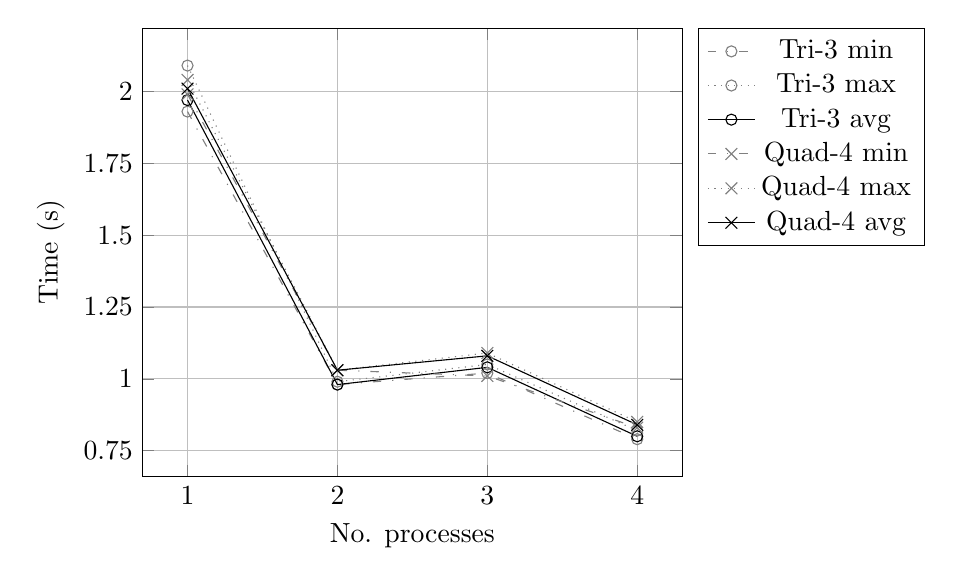
\begin{tikzpicture}
   	\begin{axis}[xlabel=No. processes,
   	ylabel=Time (s),
   	xtick={1,2,3,4},
   	ytick={2,1.75,1.5,1.25,1,0.75},
   	grid=major,
   	legend pos=outer north east]
   	\addplot[mark=o,loosely dashdotted,gray,mark options={solid}] plot coordinates {
   		(1,1.93)
   		(2,0.98)
   		(3,1.02)
   		(4,0.79)
   	};  
   	\addlegendentry{Tri-3 min}
   	\addplot[mark=o,dotted,gray,mark options={solid}] plot coordinates {
   		(1,2.09)
   		(2,0.99)
   		(3,1.05)
   		(4,0.82)
   	};  
   	\addlegendentry{Tri-3 max}
   	\addplot[mark=o,black] plot coordinates {
   		(1,1.97)
   		(2,0.98)
   		(3,1.04)
   		(4,0.8)
   	};  
   	\addlegendentry{Tri-3 avg}
   	%%%%%%%%%%%%%%%%%%%%%%%%%%%%%%%%%%%%%%%%%%%%%%%%%%%%%%%%%	
   	\addplot[mark=x,loosely dashdotted,gray,mark options={scale=1.5,solid}] plot coordinates {
   		(1,1.99)
   		(2,1.03)
   		(3,1.01)
   		(4,0.83)
   	};
   	\addlegendentry{Quad-4 min}
   	\addplot[mark=x,dotted,gray,mark options={scale=1.5,solid}] plot coordinates {
   		(1,2.04)
   		(2,1.03)
   		(3,1.09)
   		(4,0.85)
   	};
   	\addlegendentry{Quad-4 max}
   	\addplot[mark=x,black,mark options={scale=1.5}] plot coordinates {
   		(1,2.01)
   		(2,1.03)
   		(3,1.08)
   		(4,0.84)
   	};
   	\addlegendentry{Quad-4 avg}
   	\end{axis}
   	\end{tikzpicture}
   	\caption{Assembly Times}
   	\label{fig:assembly-times}
   \end{figure}
   
   \begin{figure}[htbp]
   	\centering
   	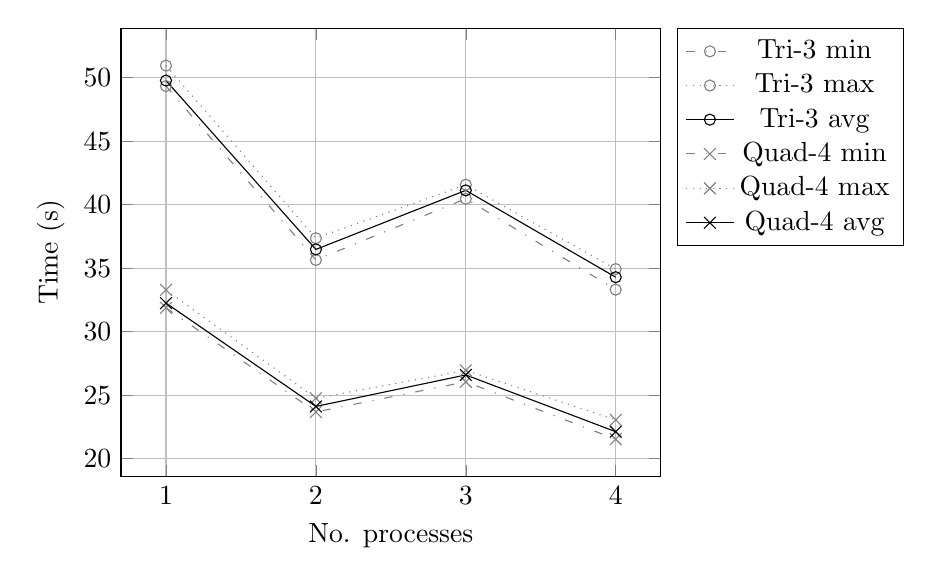
\begin{tikzpicture}
   	\begin{axis}[xlabel=No. processes,
   	ylabel=Time (s),
   	xtick={1,2,3,4},
   	ytick={50,45,40,35,30,25,20},
   	grid=major,
   	legend pos=outer north east]
   	\addplot[mark=o,loosely dashdotted,gray,mark options={solid}] plot coordinates {
   		(1,49.35)
   		(2,35.65)
   		(3,40.47)
   		(4,33.31)
   	};  
   	\addlegendentry{Tri-3 min}
   	\addplot[mark=o,dotted,gray,mark options={solid}] plot coordinates {
   		(1,50.96)
   		(2,37.36)
   		(3,41.57)
   		(4,34.93)
   	};  
   	\addlegendentry{Tri-3 max}
   	\addplot[mark=o,black] plot coordinates {
   		(1,49.78)
   		(2,36.48)
   		(3,41.13)
   		(4,34.29)
   	};  
   	\addlegendentry{Tri-3 avg}
   	%%%%%%%%%%%%%%%%%%%%%%%%%%%%%%%%%%%%%%%%%%%%%%%%%%%%%%%%%	
   	\addplot[mark=x,loosely dashdotted,gray,mark options={scale=1.5,solid}] plot coordinates {
   		(1,31.88)
   		(2,23.67)
   		(3,26.05)
   		(4,21.53)
   	};
   	\addlegendentry{Quad-4 min}
   	\addplot[mark=x,dotted,gray,mark options={scale=1.5,solid}] plot coordinates {
   		(1,33.29)
   		(2,24.75)
   		(3,26.95)
   		(4,23.05)
   	};
   	\addlegendentry{Quad-4 max}
   	\addplot[mark=x,black,mark options={scale=1.5}] plot coordinates {
   		(1,32.25)
   		(2,24.11)
   		(3,26.59)
   		(4,22.12)
   	};
   	\addlegendentry{Quad-4 avg}
   	\end{axis}
   	\end{tikzpicture}
   	\caption{Solver Times}
   	\label{fig:solver-times}
   \end{figure}
   
   \begin{figure}[htbp]
   	\centering
   	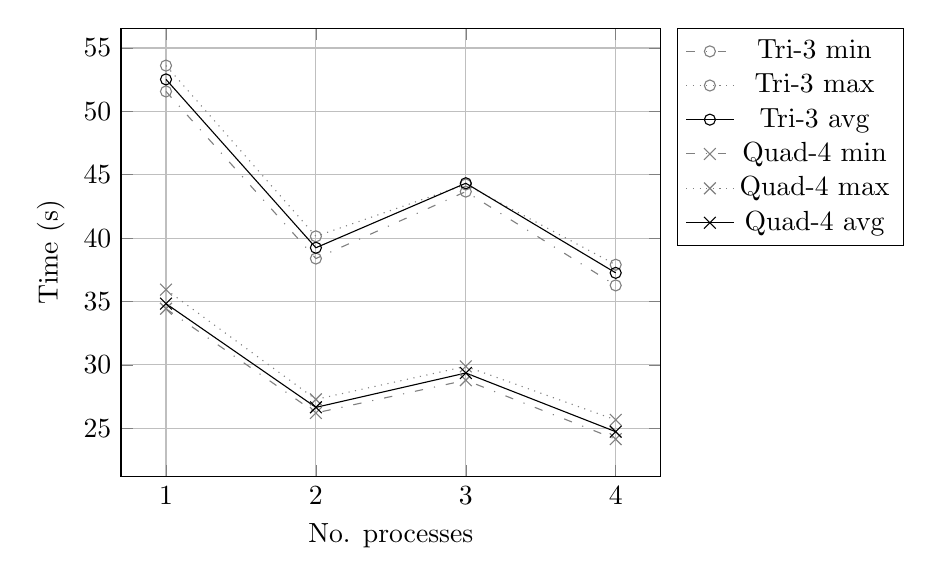
\begin{tikzpicture}
   	\begin{axis}[xlabel=No. processes,
   	ylabel=Time (s),
   	xtick={1,2,3,4},
   	ytick={55,50,45,40,35,30,25},
   	grid=major,
   	legend pos=outer north east]
   	\addplot[mark=o,loosely dashdotted,gray,mark options={solid}] plot coordinates {
   		(1,51.57)
   		(2,38.39)
   		(3,43.67)
   		(4,36.27)
   	};  
   	\addlegendentry{Tri-3 min}
   	\addplot[mark=o,dotted,gray,mark options={solid}] plot coordinates {
   		(1,53.61)
   		(2,40.14)
   		(3,44.23)
   		(4,37.90)
   	};  
   	\addlegendentry{Tri-3 max}
   	\addplot[mark=o,black] plot coordinates {
   		(1,52.52)
   		(2,39.24)
   		(3,44.33)
   		(4,37.26)
   	};  
   	\addlegendentry{Tri-3 avg}
   	%%%%%%%%%%%%%%%%%%%%%%%%%%%%%%%%%%%%%%%%%%%%%%%%%%%%%%%%%	
   	\addplot[mark=x,loosely dashdotted,gray,mark options={scale=1.5,solid}] plot coordinates {
   		(1,34.43)
   		(2,26.21)
   		(3,28.79)
   		(4,24.14)
   	};
   	\addlegendentry{Quad-4 min}
   	\addplot[mark=x,dotted,gray,mark options={scale=1.5,solid}] plot coordinates {
   		(1,35.94)
   		(2,27.28)
   		(3,29.88)
   		(4,25.66)
   	};
   	\addlegendentry{Quad-4 max}
   	\addplot[mark=x,black,mark options={scale=1.5}] plot coordinates {
   		(1,34.83)
   		(2,26.65)
   		(3,29.36)
   		(4,24.73)
   	};
   	\addlegendentry{Quad-4 avg}
   	\end{axis}
   	\end{tikzpicture}
   	\caption{Overall Times}
   	\label{fig:overall-times}
   \end{figure}
 \subsection{Test H: Coupled ``Bending Tower''}\label{sec:valid-H}
  The developed program is tested in a fluid-structure interaction. In the simulation the program gets coupled with a fluid solver developed with OpenFOAM, an open-source software for computational fluid dynamics \cite{openfoam-url}. As example problem a simple channel flow around a tower-like obstacle is simulated. The geometry configuration can be seen in Figure \ref{fig:testH}. The fluid solver simulates the flow coming from the left side of the channel and moving towards the right side. The tower is placed at the bottom side of the channel and has a simply supported boundary condition at this edge. It is simulated by the thesis' program. When the flow reaches the left side of the tower, it will bend to the right side due to the force steadily increasing by the flow. The coupling interface region in this test is the left, top and right edge of the tower.
  
  \begin{figure}[htbp]
  	\centering
  	\setlength\unitlength{1.0cm}
  	\begin{picture}(11,4)
  	\thicklines
  	\put(0.3,0.3){\vector(1,0){10.5}}\put(10.9,0.2){$x$}
  	\put(0.3,0.3){\vector(0,1){3.5}}\put(0.2,3.9){$z$}
  	\linethickness{0.5mm}
  	\polygon(0.3,0.3)(0.3,3)(10.3,3)(10.3,0.3)
  	\thicklines
  	\polyline(3.3,0.3)(3.3,1.634)(4,1.634)(4,0.3)  	
  	\thinlines
  	\polygon(3.3,0.3)(3.15,0.15)(3.45,0.15)\polygon(4,0.3)(3.85,0.15)(4.15,0.15)
  	\multiput(0.5,0.6)(0,0.5){5}{\vector(1,0){0.5}}
  	\multiput(9.6,0.6)(0,0.5){5}{\vector(1,0){0.5}}
  	
  	{\scriptsize \put(-0.15,2.9){$0.4$}\put(-0.15,1.53){$0.2$}
  		\put(0.05,0.05){$0$}
  		\put(3.05,-0.14){$0.45$}\put(3.77,-0.14){$0.55$}\put(10.12,-0.14){$1.5$}}
  	\end{picture}
  	\caption{Sketch of the ``Bending Tower'' example. An rectangular obstacle is put into a channel and flow is driven from the left side towords the right side where it leaves the fluid domain. The tower-like obstacle is represented by the structure mesh, the channel by the fluid mesh.}
  	\label{fig:testH}
  \end{figure}
  \begin{itemize}
  	\item \textbf{Mesh dimensions}\\
  	Tower height $h_t = 0.2$\\
  	Tower length $l_t = 0.1$\\
  	Tower thickness $t = 0.01$\\
  	Channel height $h_c = 0.4$\\
  	Channel length $l_c = 1.5$  	
  	
  	\item \textbf{Material properties}\\
  	Young's Modulus $E = 1.0 \times 10^4$\\
  	Poisson's ratio $\nu = 0.4$
  	
  	\item \textbf{Boundary conditions}\\
  	The bottom side of the tower is simply supported.
  	
  \end{itemize}
  
  \paragraph{Results:} 
  \begin{table}[htbp]
  	\centering
  	\begin{tabular}{C{2.3cm}|C{2.7cm}|C{1.8cm}}
  		\small\textbf{Displacement} & \small\textbf{Results from program} & \small\textbf{Difference (\%)}\\\hline\hline
  	\end{tabular}
  	\caption{Displacements and deviations for Test H}
  	\label{tab:testH}
  \end{table}
\newpage
\cleardoublepage

\section{Conclusion}
What does my code do, what problems arose, what problems persist, what does my code cannot do, where are opportunities for extensions, etc.
 \subsection{Future Work}
  \begin{itemize}
  	\item Now: Only forces at nodes are accepted and processed. Then: Pressures linked to faces can be accepted, too. The conversion to nodal values takes place in the structure solver. (Idea from coupling data mapping)
  \end{itemize}
\newpage

%\bibliographystyle{ieeetr}
\bibliographystyle{alpha}
\bibliography{thesis} %TODO preCICE paper eintrag vervollständigen
%\printbibliography

All URLs were lastly checked at December 8, 2015.
\cleardoublepage

\Affirmation
\end{document}